\documentclass[11pt,a4paper,oneside]{report}             % Single-side
%\documentclass[11pt,a4paper,twoside,openright]{report}  % Duplex
% !TEX root = ./thesis.tex  


% thanks to http://tex.stackexchange.com/a/47579/71109
\usepackage{ifxetex}
\usepackage{ifluatex}
\newif\ifxetexorluatex % a new conditional starts as false
\ifnum 0\ifxetex 1\fi\ifluatex 1\fi>0
   \xetexorluatextrue
\fi

\ifxetexorluatex
  \usepackage{fontspec}
\else
  \usepackage[T1]{fontenc}
  \usepackage[utf8]{inputenc}
  \usepackage[lighttt]{lmodern}
  \ttfamily\DeclareFontShape{T1}{lmtt}{m}{it}{<->sub*lmtt/m/sl}{}
\fi

\usepackage[english,magyar]{babel} % Alapértelmezés szerint utoljára definiált nyelv lesz aktív, de később külön beállítjuk az aktív nyelvet.

\usepackage{emptypage} % omit page number on empty pages

%\usepackage{cmap}
\usepackage{amsfonts,amsmath,amssymb} % Mathematical symbols.
%\usepackage[ruled,boxed,resetcount,linesnumbered]{algorithm2e} % For pseudocodes. % beware: this is not compatible with LuaLaTeX, see http://tex.stackexchange.com/questions/34814/lualatex-and-algorithm2e
\usepackage{booktabs} % For publication quality tables for LaTeX
\usepackage{graphicx}

%\usepackage{fancyhdr}
%\usepackage{lastpage}

\usepackage{geometry}
%\usepackage{sectsty}
\usepackage{setspace} % For setting line spacing

\usepackage[unicode]{hyperref} % For hyperlinks in the generated document.
\usepackage{xcolor}
\usepackage{listings} % For source code snippets.

\usepackage[amsmath,thmmarks]{ntheorem} % Theorem-like environments.

\usepackage[hang]{caption}

\singlespacing

\newcommand{\selecthungarian}{
	\selectlanguage{magyar}
	\setlength{\parindent}{2em}
	\setlength{\parskip}{0em}
	\frenchspacing
}

\newcommand{\selectenglish}{
	\selectlanguage{english}
	\setlength{\parindent}{0em}
	\setlength{\parskip}{0.5em}
	\nonfrenchspacing
	\renewcommand{\figureautorefname}{Figure}
	\renewcommand{\tableautorefname}{Table}
	\renewcommand{\partautorefname}{Part}
	\renewcommand{\chapterautorefname}{Chapter}
	\renewcommand{\sectionautorefname}{Section}
	\renewcommand{\subsectionautorefname}{Section}
	\renewcommand{\subsubsectionautorefname}{Section}
}

\usepackage[numbers]{natbib}
\usepackage{xspace}
\usepackage{subcaption}
\usepackage{float}
\usepackage{array}
\usepackage{tabularx}
\usepackage{cases}
\usepackage{makecell}



%TODO Set the main variables
\newcommand{\vikszerzoVezeteknev}{Jedla}
\newcommand{\vikszerzoKeresztnev}{Martin}

\newcommand{\vikkonzulensAMegszolitas}{dr.~}
\newcommand{\vikkonzulensAVezeteknev}{Bank}
\newcommand{\vikkonzulensAKeresztnev}{Balázs}

\newcommand{\vikkonzulensBMegszolitas}{}
\newcommand{\vikkonzulensBVezeteknev}{}
\newcommand{\vikkonzulensBKeresztnev}{}

\newcommand{\vikkonzulensCMegszolitas}{}
\newcommand{\vikkonzulensCVezeteknev}{}
\newcommand{\vikkonzulensCKeresztnev}{}

\newcommand{\vikcim}{Gitárerősítő valós idejű modellezése K-módszerrel} % Cím
\newcommand{\viktanszek}{\bmemit} % Tanszék
\newcommand{\vikdoktipus}{\bsconlab} % Dokumentum típusa (\bsc vagy \msc)
\newcommand{\vikmunkatipusat}{szakdolgozatot} % a "hallgató nyilatkozat" részhez: szakdolgozatot vagy diplomatervet

%--------------------------------------------------------------------------------------
% TDK-specifikus változók
%--------------------------------------------------------------------------------------
\newcommand{\tdkszerzoB}{} % Második szerző neve; hagyd üresen, ha egyedül írtad a TDK-t.
\newcommand{\tdkev}{2024} % A dolgozat írásának éve (pl. "2014") (Ez OTDK-nál eltérhet az aktuális évtől.)

% További adatok az OTDK címlaphoz (BME-s TDK-hoz nem kell kitölteni)
\newcommand{\tdkevfolyamA}{IV} % Első szerző évfolyama, római számmal (pl. IV).
\newcommand{\tdkevfolyamB}{} % Második szerző évfolyama, római számmal (pl. III).
\newcommand{\tdkkonzulensbeosztasA}{egyetemi docens} % Első konzulens beosztása (pl. egyetemi docens)
\newcommand{\tdkkonzulensbeosztasB}{} % Második konzulens beosztása (pl. egyetemi docens)

\newcommand{\szerzoMeta}{\vikszerzoVezeteknev{} \vikszerzoKeresztnev} % egy szerző esetén
%\newcommand{\szerzoMeta}{\vikszerzoVezeteknev{} \vikszerzoKeresztnev, \tdkszerzoB} % két szerző esetén

%TODO Language configuration -- choose one
% Beállítások magyar nyelvű dolgozathoz
%--------------------------------------------------------------------------------------
% Elnevezések
%--------------------------------------------------------------------------------------
\newcommand{\bme}{Budapesti Műszaki és Gazdaságtudományi Egyetem}
\newcommand{\vik}{Villamosmérnöki és Informatikai Kar}

\newcommand{\bmemit}{Méréstechnika és Információs Rendszerek Tanszék}

\newcommand{\keszitette}{Készítette}
\newcommand{\konzulens}{Konzulens}

\newcommand{\bsc}{Szakdolgozat}
\newcommand{\msc}{Diplomaterv}
\newcommand{\tdk}{TDK dolgozat}
\newcommand{\bsctemalab}{BSc Témalaboratórium}
\newcommand{\bsconlab}{BSc Önálló laboratórium}
\newcommand{\msconlabi}{MSc Önálló laboratórium 1.}
\newcommand{\msconlabii}{MSc Önálló laboratórium 2.}

\newcommand{\pelda}{Példa}
\newcommand{\definicio}{Definíció}
\newcommand{\tetel}{Tétel}

\newcommand{\bevezetes}{Bevezetés}
\newcommand{\koszonetnyilvanitas}{Köszönetnyilvánítás}
\newcommand{\fuggelek}{Függelék}

% Opcionálisan átnevezhető címek
%\addto\captionsmagyar{%
%\renewcommand{\listfigurename}{Saját ábrajegyzék cím}
%\renewcommand{\listtablename}{Saját táblázatjegyzék cím}
%\renewcommand{\bibname}{Saját irodalomjegyzék név}
%}

\newcommand{\szerzo}{\vikszerzoVezeteknev{} \vikszerzoKeresztnev}
\newcommand{\vikkonzulensA}{\vikkonzulensAMegszolitas\vikkonzulensAVezeteknev{} \vikkonzulensAKeresztnev}
\newcommand{\vikkonzulensB}{\vikkonzulensBMegszolitas\vikkonzulensBVezeteknev{} \vikkonzulensBKeresztnev}
\newcommand{\vikkonzulensC}{\vikkonzulensCMegszolitas\vikkonzulensCVezeteknev{} \vikkonzulensCKeresztnev}

\newcommand{\selectthesislanguage}{\selecthungarian}

\bibliographystyle{huplain}

\def\lstlistingname{lista}

\newcommand{\appendixnumber}{6}  % a fofejezet-szamlalo az angol ABC 6. betuje (F) lesz

% Settings for English documents
%%--------------------------------------------------------------------------------------
% Elnevezések
%--------------------------------------------------------------------------------------
\newcommand{\bme}{Budapest University of Technology and Economics}
\newcommand{\vik}{Faculty of Electrical Engineering and Informatics}

\newcommand{\bmemit}{Department of Measurement and Information Systems}

\newcommand{\keszitette}{Author}
\newcommand{\konzulens}{Advisor}

\newcommand{\bsc}{Bachelor's Thesis}
\newcommand{\msc}{Master's Thesis}
\newcommand{\tdk}{Scientific Students' Association Report}
\newcommand{\bsconlab}{BSc Project Laboratory}
\newcommand{\msconlabi}{MSc Project Laboratory 1}
\newcommand{\msconlabii}{MSc Project Laboratory 2}

\newcommand{\pelda}{Example}
\newcommand{\definicio}{Definition}
\newcommand{\tetel}{Theorem}

\newcommand{\bevezetes}{Introduction}
\newcommand{\koszonetnyilvanitas}{Acknowledgements}
\newcommand{\fuggelek}{Appendix}

% Optional custom titles
%\addto\captionsenglish{%
%\renewcommand*{\listfigurename}{Your list of figures title}
%\renewcommand*{\listtablename}{Your list of tables title}
%\renewcommand*{\bibname}{Your bibliography title}
%}

\newcommand{\szerzo}{\vikszerzoKeresztnev{} \vikszerzoVezeteknev}
\newcommand{\vikkonzulensA}{\vikkonzulensAMegszolitas\vikkonzulensAKeresztnev{} \vikkonzulensAVezeteknev}
\newcommand{\vikkonzulensB}{\vikkonzulensBMegszolitas\vikkonzulensBKeresztnev{} \vikkonzulensBVezeteknev}
\newcommand{\vikkonzulensC}{\vikkonzulensCMegszolitas\vikkonzulensCKeresztnev{} \vikkonzulensCVezeteknev}

\newcommand{\selectthesislanguage}{\selectenglish}

\bibliographystyle{plainnat}

\newcommand{\ie}{i.e.\@\xspace}
\newcommand{\Ie}{I.e.\@\xspace}
\newcommand{\eg}{e.g.\@\xspace}
\newcommand{\Eg}{E.g.\@\xspace}
\newcommand{\etal}{et al.\@\xspace}
\newcommand{\etc}{etc.\@\xspace}
\newcommand{\vs}{vs.\@\xspace}
\newcommand{\viz}{viz.\@\xspace} % videlicet
\newcommand{\cf}{cf.\@\xspace} % confer
\newcommand{\Cf}{Cf.\@\xspace}
\newcommand{\wrt}{w.r.t.\@\xspace} % with respect to
\newcommand{\approximately}{approx.\@\xspace}

\newcommand{\appendixnumber}{1}  % a fofejezet-szamlalo az angol ABC 1. betuje (A) lesz


%--------------------------------------------------------------------------------------
% Page layout setup
%--------------------------------------------------------------------------------------
% we need to redefine the pagestyle plain
% another possibility is to use the body of this command without \fancypagestyle
% and use \pagestyle{fancy} but in that case the special pages
% (like the ToC, the References, and the Chapter pages)remain in plane style

\pagestyle{plain}
\geometry{inner=35mm, outer=25mm, top=28mm, bottom=25mm}

\setcounter{tocdepth}{3}
%\sectionfont{\large\upshape\bfseries}
\setcounter{secnumdepth}{3}

\sloppy % Margón túllógó sorok tiltása.
\widowpenalty=10000 \clubpenalty=10000 %A fattyú- és árvasorok elkerülése
\def\hyph{-\penalty0\hskip0pt\relax} % Kötőjeles szavak elválasztásának engedélyezése


%--------------------------------------------------------------------------------------
% Setup hyperref package
%--------------------------------------------------------------------------------------
\hypersetup{
    % bookmarks=true,            % show bookmarks bar?
    unicode=true,              % non-Latin characters in Acrobat's bookmarks
    pdftitle={\vikcim},        % title
    pdfauthor={\szerzoMeta},    % author
    pdfsubject={\vikdoktipus}, % subject of the document
    pdfcreator={\szerzoMeta},   % creator of the document
    pdfproducer={},    % producer of the document
    pdfkeywords={},    % list of keywords (separate then by comma)
    pdfnewwindow=true,         % links in new window
    colorlinks=true,           % false: boxed links; true: colored links
    linkcolor=black,           % color of internal links
    citecolor=black,           % color of links to bibliography
    filecolor=black,           % color of file links
    urlcolor=black             % color of external links
}


%--------------------------------------------------------------------------------------
% Set up listings
%--------------------------------------------------------------------------------------
\definecolor{lightgray}{rgb}{0.95,0.95,0.95}
\lstset{
	basicstyle=\scriptsize\ttfamily, % print whole listing small
	keywordstyle=\color{black}\bfseries, % bold black keywords
	identifierstyle=, % nothing happens
	% default behavior: comments in italic, to change use
	% commentstyle=\color{green}, % for e.g. green comments
	stringstyle=\scriptsize,
	showstringspaces=false, % no special string spaces
	aboveskip=3pt,
	belowskip=3pt,
	backgroundcolor=\color{lightgray},
	columns=flexible,
	keepspaces=true,
	escapeinside={(*@}{@*)},
	captionpos=b,
	breaklines=true,
	frame=single,
	float=!ht,
	tabsize=2,
	literate=*
		{á}{{\'a}}1	{é}{{\'e}}1	{í}{{\'i}}1	{ó}{{\'o}}1	{ö}{{\"o}}1	{ő}{{\H{o}}}1	{ú}{{\'u}}1	{ü}{{\"u}}1	{ű}{{\H{u}}}1
		{Á}{{\'A}}1	{É}{{\'E}}1	{Í}{{\'I}}1	{Ó}{{\'O}}1	{Ö}{{\"O}}1	{Ő}{{\H{O}}}1	{Ú}{{\'U}}1	{Ü}{{\"U}}1	{Ű}{{\H{U}}}1
}


%--------------------------------------------------------------------------------------
% Set up theorem-like environments
%--------------------------------------------------------------------------------------
% Using ntheorem package -- see http://www.math.washington.edu/tex-archive/macros/latex/contrib/ntheorem/ntheorem.pdf

\theoremstyle{plain}
\theoremseparator{.}
\newtheorem{example}{\pelda}

\theoremseparator{.}
%\theoremprework{\bigskip\hrule\medskip}
%\theorempostwork{\hrule\bigskip}
\theorembodyfont{\upshape}
\theoremsymbol{{\large \ensuremath{\centerdot}}}
\newtheorem{definition}{\definicio}

\theoremseparator{.}
%\theoremprework{\bigskip\hrule\medskip}
%\theorempostwork{\hrule\bigskip}
\newtheorem{theorem}{\tetel}


%--------------------------------------------------------------------------------------
% Some new commands and declarations
%--------------------------------------------------------------------------------------
\newcommand{\code}[1]{{\upshape\ttfamily\scriptsize\indent #1}}
\newcommand{\doi}[1]{DOI: \href{http://dx.doi.org/\detokenize{#1}}{\raggedright{\texttt{\detokenize{#1}}}}} % A hivatkozások közt így könnyebb DOI-t megadni.

\DeclareMathOperator*{\argmax}{arg\,max}
%\DeclareMathOperator*[1]{\floor}{arg\,max}
\DeclareMathOperator{\sign}{sgn}
\DeclareMathOperator{\rot}{rot}


%--------------------------------------------------------------------------------------
% Setup captions
%--------------------------------------------------------------------------------------
\captionsetup[figure]{aboveskip=10pt}

\renewcommand{\captionlabelfont}{\bf}
%\renewcommand{\captionfont}{\footnotesize\it}

%--------------------------------------------------------------------------------------
% Hyphenation exceptions
%--------------------------------------------------------------------------------------
\hyphenation{Shakes-peare Mar-seilles ár-víz-tű-rő tü-kör-fú-ró-gép}


\author{\vikszerzo}
\title{\viktitle}


%--------------------------------------------------------------------------------------
% Table of contents and the main text
%--------------------------------------------------------------------------------------
\begin{document}

\pagenumbering{gobble}

%TODO These includes define guidelines -- remove these
%~~~~~~~~~~~~~~~~~~~~~~~~~~~~~~~~~~~~~~~~~~~~~~~~~~~~~~~~~~~~~~~~~~~~~~~~~~~~~~~~~~~~~~
%\selecthungarian
%--------------------------------------------------------------------------------------
% Rovid formai es tartalmi tajekoztato
%--------------------------------------------------------------------------------------

\footnotesize
\begin{center}
\large
\textbf{\Large Általános információk, a diplomaterv szerkezete}\\
\end{center}

A diplomaterv szerkezete a BME Villamosmérnöki és Informatikai Karán:
\begin{enumerate}
\item	Diplomaterv feladatkiírás
\item	Címoldal
\item	Tartalomjegyzék
\item	A diplomatervező nyilatkozata az önálló munkáról és az elektronikus adatok kezeléséről
\item	Tartalmi összefoglaló magyarul és angolul
\item	Bevezetés: a feladat értelmezése, a tervezés célja, a feladat indokoltsága, a diplomaterv felépítésének rövid összefoglalása
\item	A feladatkiírás pontosítása és részletes elemzése
\item	Előzmények (irodalomkutatás, hasonló alkotások), az ezekből levonható következtetések
\item	A tervezés részletes leírása, a döntési lehetőségek értékelése és a választott megoldások indoklása
\item	A megtervezett műszaki alkotás értékelése, kritikai elemzése, továbbfejlesztési lehetőségek
\item	Esetleges köszönetnyilvánítások
\item	Részletes és pontos irodalomjegyzék
\item	Függelék(ek)
\end{enumerate}

Felhasználható a következő oldaltól kezdődő \LaTeX diplomatervsablon dokumentum tartalma. 

A diplomaterv szabványos méretű A4-es lapokra kerüljön. Az oldalak tükörmargóval készüljenek (mindenhol 2,5~cm, baloldalon 1~cm-es kötéssel). Az alapértelmezett betűkészlet a 12 pontos Times New Roman, másfeles sorközzel, de ettől kismértékben el lehet térni, ill. más betűtípus használata is megengedett.

Minden oldalon -- az első négy szerkezeti elem kivételével -- szerepelnie kell az oldalszámnak.

A fejezeteket decimális beosztással kell ellátni. Az ábrákat a megfelelő helyre be kell illeszteni, fejezetenként decimális számmal és kifejező címmel kell ellátni. A fejezeteket decimális aláosztással számozzuk, maximálisan 3 aláosztás mélységben (pl. 2.3.4.1.). Az ábrákat, táblázatokat és képleteket célszerű fejezetenként külön számozni (pl. 2.4. ábra, 4.2. táblázat vagy képletnél (3.2)). A fejezetcímeket igazítsuk balra, a normál szövegnél viszont használjunk sorkiegyenlítést. Az ábrákat, táblázatokat és a hozzájuk tartozó címet igazítsuk középre. A cím a jelölt rész alatt helyezkedjen el.

A képeket lehetőleg rajzoló programmal készítsék el, az egyenleteket egyenlet-szerkesztő segítségével írják le (A \LaTeX~ehhez kézenfekvő megoldásokat nyújt).

Az irodalomjegyzék szövegközi hivatkozása történhet sorszámozva (ez a preferált megoldás) vagy a Harvard-rendszerben (a szerző és az évszám megadásával). A teljes lista névsor szerinti sorrendben a szöveg végén szerepeljen (sorszámozott irodalmi hivatkozások esetén hivatkozási sorrendben). A szakirodalmi források címeit azonban mindig az eredeti nyelven kell megadni, esetleg zárójelben a fordítással. A listában szereplő valamennyi publikációra hivatkozni kell a szövegben (a \LaTeX-sablon a Bib\TeX~segítségével mindezt automatikusan kezeli). Minden publikáció a szerzők után a következő adatok szerepelnek: folyóirat cikkeknél a pontos cím, a folyóirat címe, évfolyam, szám, oldalszám tól-ig. A folyóiratok címét csak akkor rövidítsük, ha azok nagyon közismertek vagy nagyon hosszúak. Internetes hivatkozások megadásakor fontos, hogy az elérési út előtt megadjuk az oldal tulajdonosát és tartalmát (mivel a link egy idő után akár elérhetetlenné is válhat), valamint az elérés időpontját.

\vspace{5mm}
Fontos:
\begin{itemize}
	\item A szakdolgozatkészítő / diplomatervező nyilatkozata (a jelen sablonban szereplő szövegtartalommal) kötelező előírás, Karunkon ennek hiányában a szakdolgozat/diplomaterv nem bírálható és nem védhető!
	\item Mind a dolgozat, mind a melléklet maximálisan 15~MB méretű lehet!
\end{itemize}

\vspace{5mm}
\begin{center}
Jó munkát, sikeres szakdolgozatkészítést, ill. diplomatervezést kívánunk!
\end{center}

\normalsize
\selectthesislanguage

%%--------------------------------------------------------------------------------------
% Feladatkiiras (a tanszeken atveheto, kinyomtatott valtozat)
%--------------------------------------------------------------------------------------
\clearpage
\begin{center}
\large
\textbf{FELADATKIÍRÁS}\\
\end{center}

A feladatkiírást a tanszéki adminisztrációban lehet átvenni, és a leadott munkába eredeti, tanszéki pecséttel ellátott és a tanszékvezető által aláírt lapot kell belefűzni (ezen oldal \emph{helyett}, ez az oldal csak útmutatás). Az elektronikusan feltöltött dolgozatban már nem kell beleszerkeszteni ezt a feladatkiírást.


\selectthesislanguage

%TODO Titlepage -- choose one from below
%~~~~~~~~~~~~~~~~~~~~~~~~~~~~~~~~~~~~~~~~~~~~~~~~~~~~~~~~~~~~~~~~~~~~~~~~~~~~~~~~~~~~~~
%\hypersetup{pageanchor=false}
%--------------------------------------------------------------------------------------
%	The title page
%--------------------------------------------------------------------------------------
\begin{titlepage}
\begin{center}
\includegraphics[width=60mm,keepaspectratio]{figures/bme_logo.pdf}\\
\vspace{0.3cm}
\textbf{\bme}\\
\textmd{\vik}\\
\textmd{\viktanszek}\\[5cm]

\vspace{0.4cm}
{\huge \bfseries \vikcim}\\[0.8cm]
\vspace{0.5cm}
\textsc{\Large \vikdoktipus}\\[4cm]

{
	\renewcommand{\arraystretch}{0.85}
	\begin{tabular}{cc}
	 \makebox[7cm]{\emph{\keszitette}} & \makebox[7cm]{\emph{\konzulens}} \\ \noalign{\smallskip}
	 \makebox[7cm]{\szerzo} & \makebox[7cm]{\vikkonzulensA} \\
	  & \makebox[7cm]{\vikkonzulensB} \\
	  & \makebox[7cm]{\vikkonzulensC} \\
	\end{tabular}
}

\vfill
{\large 2024}
\end{center}
\end{titlepage}
\hypersetup{pageanchor=false}

		   % Szakdolgozat/Diplomaterv címlap
%% TDK címlap
\begin{titlepage}
  \begin{center}  
  \includegraphics[width=7cm]{./figures/bme_logo.pdf}
  \vspace{0.3cm}
  
  \bme \\
  \vik \\
  \viktanszek \\
  \vspace{5cm}
  
  \huge {\vikcim}
  \vspace{1.5cm}
  
  \large {\textbf{\tdk}}
  \vfill
    
  {\Large 
  	\keszitette: \\ \vspace{0.3cm}
  	\szerzo \\
	%\tdkszerzoB \\
  	\vspace{1.5cm}
  	\konzulens: \\ \vspace{0.3cm}
  	\vikkonzulensA \\
  	%\vikkonzulensB \\
  }
  
  \vspace{2cm}
  \large {\tdkev}
 \end{center}
\end{titlepage}
%% Címlap vége
	% TDK címlap
%%% OTDK külső címlap
\begin{titlepage}
  	$\;$ 
	\vspace{5cm}
	
	\begin{center}
	\Huge
	\textbf{TDK-dolgozat}\let\thefootnote\relax\footnote{A dolgozat bemutatását a XXXXXXXXX  ``Lorem ipsum dolor sit amet'' című program támogatta.}
	\end{center}
	
	\vspace{13cm}
	
	\Large
	\hspace{8cm} \szerzo
	
	\hspace{8cm} \tdkszerzoB
	
	\hspace{8cm} \tdkev.
\end{titlepage}

\newpage
\thispagestyle{empty}


%% OTDK belső címlap
\begin{titlepage}
  \begin{center}  
  \includegraphics[width=7cm]{./figures/bme_logo.pdf}
  \vspace{0.3cm}
  
  \bme \\
  \vik \\
  \viktanszek \\
  \vspace{3.5cm}
  
  \huge {\vikcim}
  \vspace{1.5cm}
  
  \large {\textbf{\vikdoktipus}}
  \vfill
    
  {\Large 
  	{\large \keszitette:} \\ \vspace{0.2cm}
  	\szerzo \\ \tdkevfolyamA. évfolyam \\
	\vspace{0.5cm}
	\tdkszerzoB \\ \tdkevfolyamB. évfolyam \\
  	\vspace{1.5cm}
  	{\large \konzulens:} \\ \vspace{0.2cm}
  	\vikkonzulensA,\\ \tdkkonzulensbeosztasA \\
  	\vspace{0.5cm}
  	\vikkonzulensB,\\ \tdkkonzulensbeosztasB \\
  }
  
  \vspace{2cm}
  \large {\tdkev.}
  
 \end{center}
\end{titlepage}   % OTDK címlap


% Table of Contents
%~~~~~~~~~~~~~~~~~~~~~~~~~~~~~~~~~~~~~~~~~~~~~~~~~~~~~~~~~~~~~~~~~~~~~~~~~~~~~~~~~~~~~~
\tableofcontents\cleardoublepage


% Declaration and Abstract
%~~~~~~~~~~~~~~~~~~~~~~~~~~~~~~~~~~~~~~~~~~~~~~~~~~~~~~~~~~~~~~~~~~~~~~~~~~~~~~~~~~~~~~
%\selectlanguage{magyar}
\pagenumbering{gobble}
%--------------------------------------------------------------------------------------
% Nyilatkozat
%--------------------------------------------------------------------------------------
\begin{center}
\large
\textbf{HALLGATÓI NYILATKOZAT}\\
\end{center}

Alulírott \emph{\vikszerzoVezeteknev{} \vikszerzoKeresztnev}, szigorló hallgató kijelentem, hogy ezt a \vikmunkatipusat{} meg nem engedett segítség nélkül, saját magam készítettem, csak a megadott forrásokat (szakirodalom, eszközök stb.) használtam fel. Minden olyan részt, melyet szó szerint, vagy azonos értelemben, de átfogalmazva más forrásból átvettem, egyértelműen, a forrás megadásával megjelöltem.

Hozzájárulok, hogy a jelen munkám alapadatait (szerző(k), cím, angol és magyar nyelvű tartalmi kivonat, készítés éve, konzulens(ek) neve) a BME VIK nyilvánosan hozzáférhető elektronikus formában, a munka teljes szövegét pedig az egyetem belső hálózatán keresztül (vagy autentikált felhasználók számára) közzétegye. Kijelentem, hogy a benyújtott munka és annak elektronikus verziója megegyezik. Dékáni engedéllyel titkosított diplomatervek esetén a dolgozat szövege csak 3 év eltelte után válik hozzáférhetővé.

\begin{flushleft}
\vspace*{1cm}
Budapest, \today
\end{flushleft}

\begin{flushright}
 \vspace*{1cm}
 \makebox[7cm]{\rule{6cm}{.4pt}}\\
 \makebox[7cm]{\emph{\vikszerzoVezeteknev{} \vikszerzoKeresztnev}}\\
 \makebox[7cm]{hallgató}
\end{flushright}
\thispagestyle{empty}

\vfill
\cleardoublepage

\selectthesislanguage
 %TODO Hallgatói nyilatkozat -- TDK és OTDK esetén törlendő!
\pagenumbering{roman}
\setcounter{page}{1}

\selecthungarian

%----------------------------------------------------------------------------
% Abstract in Hungarian
%----------------------------------------------------------------------------
\chapter*{Összefoglalás}\addcontentsline{toc}{chapter}{Összefoglalás}

Napjainkban a zeneiparban és a zenészek körében a hangzás megváltoztatása céljából alkalmazott hardver-effektek helyett egyre gyakrabban használnak számítógépen futtatható pluginokat. Ezek a pluginok valós időben futnak, és gyakran a fizikai effekt áramköre alapján valósítják meg őket, lehetőleg úgy, hogy ugyanazt a hangzásélményt nyújtsák.

Ezeknek a pluginoknak az elkészítése nem triviális: a zenei eszközök áramkörében gyakran találhatóak nemlineáris elemek (diódák, elektroncsövek stb.), amelyek megnehezítik digitális modellezésüket. A valós idejűség követelménye miatt olyan módszereket kell találni, amelyek elfogadható számítási igény mellett is megfelelő pontossággal oldják meg a nemlineáris differenciálegyenlet rendszert. Ezek a módszerek jellemzően nem triviális egyszerűsítésekkel (akár az egyenletrendszer másképpen való felírásával, akár algebrai átalakítások segítségével) próbálják ezt elérni.

Nemlineáris differenciálegyenletek megoldására az egyik legegyszerűbb és leggyakrabban használt eljárások az úgynevezett Euler módszerek. Azonban az előrelépő Euler módszernél a modell stabilitása nem garantált, a hátralépő Euler módszer pedig a nemlineáris differenciálegyenlet numerikus megoldását igényli, ezzel nagy számítási igényt előidézve.

A kevésbé ismert K-módszer a számítási igényt azzal igyekszik csökkenteni, hogy az áramkör lineáris és nemlineáris részáramkörökre bontása után először a nemlineáris rész kimenetét számolja ki geometriai módszerek segítségével, majd csak ezután számolja ki a további szükséges változókat. Korábban ezt a módszert a kutatott irodalom nem hasonlította össze az más állapotteres módszerekkel. A TDK dolgozat célja a K-módszer és a hátralépő Euler módszer kapcsolódásainak vizsgálata, valamint hasonlóságaik és különbségeik feltérképezése. Emellett a dolgozat azt is részletezi, hogy milyen előnyei és hátrányai vannak a K-módszernek a hátralépő Euler-módszerrel szemben, és a lehetséges alkalmazási területeit is ismerteti.

A K-módszer bemutatásához az Orange Crush 20L gitárerősítőt modelleztem, illetve ez alapján egy valós időben futó VST3 plugint készítettem JUCE fejlesztői környezetben.\vfill
%\selectenglish


%----------------------------------------------------------------------------
% Abstract in English
%----------------------------------------------------------------------------
\chapter*{Abstract}\addcontentsline{toc}{chapter}{Abstract}
In today's music industry and among musicians, instead of using hardware effects to alter sound, digital plugins are increasingly being used. These plugins are run in real time and are mostly designed to emulate the physical circuit of the desired effect, aiming to deliver the same listening experience.

The design of these plugins is not trivial: the circuits of musical devices often contain nonlinear components (diodes, vacuum tubes, etc.), which complicates their digital modeling. Due to the real-time requirement, methods must be applied that can solve the ordinary differential equation caused by the nonlinearity with sufficient accuracy while having an acceptable computational demand. These methods typically achieve this through non-trivial simplifications (either by defining the equation system differently or through algebraic transformations).

One of the simplest and most common methods used for solving nonlinear differential equations are the so-called Euler methods. However, with the forward Euler method, the stability of the system is not guaranteed, and with the backward Euler method, the numerical solving of a nonlinear differential equation is required.

The lesser-known K-method tries to reduce the computational demand by dividing the circuit into a linear and nonlinear subsircuit. First, it calculates the output of the nonlinear part by geometric methods and only then calculates the other necessary variables. Previously, this method has not been compared to other state-space methods in the literature. The goal of this paper is to examine the connection between the K-method and the backward Euler method, as well as to detail their similarities and differences. Additionally, the paper details the advantages and disadvantages of the K-method against the backward Euler method and also outlines its possible application areas.

To demonstrate the K-method, I have modeled the Orange Crush 20L guitar amplifier, and I have programmed a VST3 plugin in the JUCE framework.
\vfill
\cleardoublepage

\selectthesislanguage

\newcounter{romanPage}
\setcounter{romanPage}{\value{page}}
\stepcounter{romanPage}    %TODO Összefoglaló -- TDK és OTDK esetén nem kötelező


% The main part of the thesis
%~~~~~~~~~~~~~~~~~~~~~~~~~~~~~~~~~~~~~~~~~~~~~~~~~~~~~~~~~~~~~~~~~~~~~~~~~~~~~~~~~~~~~~
\pagenumbering{arabic}

%TODO import your own content
%%----------------------------------------------------------------------------
\chapter{\bevezetes}
%----------------------------------------------------------------------------

A bevezető tartalmazza a diplomaterv-kiírás elemzését, történelmi előzményeit, a feladat indokoltságát (a motiváció leírását), az eddigi megoldásokat, és ennek tükrében a hallgató megoldásának összefoglalását.

A bevezető szokás szerint a diplomaterv felépítésével záródik, azaz annak rövid leírásával, hogy melyik fejezet mivel foglalkozik.

%%----------------------------------------------------------------------------
\chapter{\LaTeX-eszközök}
\label{sec:LatexTools}
%----------------------------------------------------------------------------
\section{A szerkesztéshez használatos eszközök}
%----------------------------------------------------------------------------
Ez a sablon TeXstudio 2.8.8 szerkesztővel készült. A TeXstudio egy platformfüggetlen, Windows, Linux és Mac OS alatt is elérhető \LaTeX-szerkesztőprogram számtalan hasznos szolgáltatással (\refstruc{fig:TeXstudio}). A szoftver ingyenesen letölthető\footnote{A TeXstudio hivatalos oldala: \url{http://texstudio.sourceforge.net/}}.

\begin{figure}[!ht]
\centering
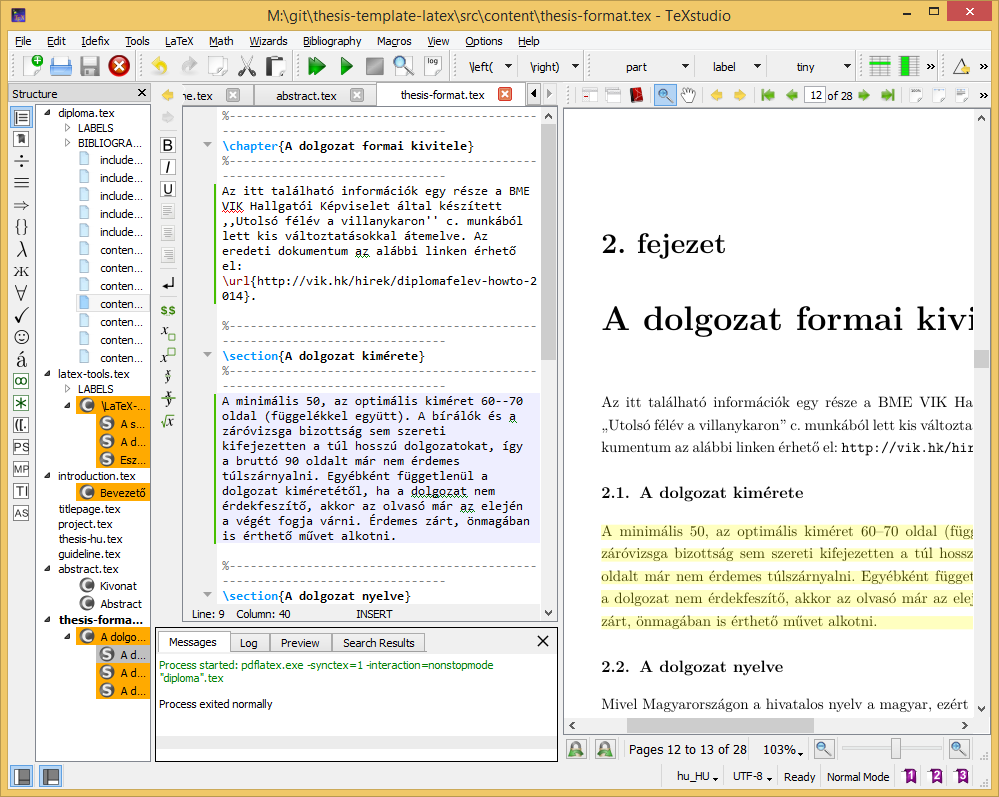
\includegraphics[width=150mm, keepaspectratio]{figures/TeXstudio.png}
\caption{A TeXstudio \LaTeX-szerkesztő.}
\label{fig:TeXstudio}
\end{figure}

A TeXstudio telepítése után érdemes még letölteni a magyar nyelvű helyesírásellenőrző-szótárakat hozzá. A TeXstudio az OpenOffice-hoz használatos formátumot tudja kezelni. A TeXstudio beállításainál a \verb+General+ fülön a \verb+Dictionaries+ résznél tudjuk megadni, hogy melyik szótárat használja.

Egy másik használható Windows alapú szerkesztőprogram a LEd\footnote{A LEd hivatalos oldala: \url{http://www.latexeditor.org/}} (LaTeX Editor), a TeXstudio azonban stabilabb, gyorsabb, és jobban használható.

%----------------------------------------------------------------------------
\section{A dokumentum lefordítása Windows alatt}
%----------------------------------------------------------------------------
A TeXstudio és a LEd kizárólag szerkesztőprogram (bár az utóbbiban DVI-nézegető is van), így a dokumentum fordításához szükséges eszközöket nem tartalmazza. Windows alatt alapvetően két lehetőség közül érdemes választani: MiKTeX (\url{http://miktex.org/}) és TeX Live (\url{http://www.tug.org/texlive/}) programcsomag. Az utóbbi működik Mac OS X, GNU/Linux alatt és Unix-származékokon is. A MiKTeX egy alapcsomag telepítése után mindig letölti a használt funkciókhoz szükséges, de lokálisan hiányzó \TeX-csomagokat, míg a TeX Live DVD ISO verzóban férhető hozzá. Ez a dokumentum TeX Live 2008 programcsomag segítségével fordult, amelynek DVD ISO verziója a megadott oldalról letölthető. A sablon lefordításához a disztribúcióban szereplő \verb+magyar.ldf+ fájlt a \verb+http://www.math.bme.hu/latex/+ változatra kell cserélni, vagy az utóbbi változatot be kell másolni a projekt-könyvtárba (ahogy ezt meg is tettük a sablonban) különben anomáliák tapasztalhatók a dokumentumban (pl. az ábra- és táblázat-aláírások formátuma nem a beállított lesz, vagy bizonyos oldalakon megjelenik alapértelmezésben egy fejléc). A TeX Live 2008-at még nem kell külön telepíteni a gépre, elegendő DVD-ről (vagy az ISO fájlból közvetlenül, pl. DaemonTools-szal) használni.

Ha a MiKTeX csomagot használjuk, akkor parancssorból a következő módon tudjuk újrafordítani a teljes dokumentumot:

\begin{lstlisting}[language=bash,frame=single,float=!ht]
$ texify -p thesis.tex
\end{lstlisting}

A \verb+texify+ parancs a MiKTex programcsomag \verb+miktex/bin+ alkönyvtárában található. A parancs gondoskodik arról, hogy a szükséges lépéseket (fordítás, hivatkozások generálása stb.) a megfelelő sorrendben elvégezze. A \verb+-p+ kapcsoló hatására PDF-et generál. A fordítást és az ideiglenes fájlok törlését elvégezhetjük a sablonhoz mellékelt \verb+manual_build.bat+ szkript segítségével is.

A \TeX-eszközöket tartalmazó programcsomag binárisainak elérési útját gyakran be kell állítani a szerkesztőprogramban, például TeXstudio esetén legegyszerűbben az \verb+Options / Configure TeXstudio... / Commands+ menüponttal előhívott dialógusablakban tehetjük ezt meg.

A PDF-\LaTeX~használata esetén a generált dokumentum közvetlenül PDF-formátumban áll rendelkezésre. Amennyiben a PDF-fájl egy PDF-nézőben (pl. Adobe Acrobat Reader vagy Foxit PDF Reader) meg van nyitva, akkor a fájlleírót a PDF-néző program tipikusan lefoglalja. Ilyen esetben a dokumentum újrafordítása hibaüzenettel kilép. Ha bezárjuk és újra megnyitjuk a PDF dokumentumot, akkor pedig a PDF-nézők többsége az első oldalon nyitja meg a dokumentumot, nem a legutóbb olvasott oldalon. Ezzel szemben például az egyszerű és ingyenes \textcolor{blue}{Sumatra PDF} nevű program képes arra, hogy a megnyitott dokumentum megváltozását detektálja, és frissítse a nézetet az aktuális oldal megtartásával.

%----------------------------------------------------------------------------
\section{Eszközök Linuxhoz}
%----------------------------------------------------------------------------
Linux operációs rendszer alatt is rengeteg szerkesztőprogram van, pl. a KDE alapú Kile jól használható. Ez ingyenesen letölthető, vagy éppenséggel az adott Linux-disztribúció eleve tartalmazza, ahogyan a dokumentum fordításához szükséges csomagokat is. Az Ubuntu Linux disztribúciók alatt például legtöbbször a \verb+texlive-*+ csomagok telepítésével használhatók a \LaTeX-eszközök. A jelen sablon fordításához szükséges csomagok (kb. 0,5 GB) az alábbi paranccsal telepíthetők:

\begin{lstlisting}[language=bash,morekeywords={sudo,apt\-get},alsoletter={-},breaklines=true]
$ sudo apt-get install texlive-latex-extra texlive-fonts-extra texlive-fonts-recommended texlive-lang-european texlive-xetex texlive-science
\end{lstlisting}

Amennyiben egy újabb csomag hozzáadása után hiányzó fájlra utaló hibát kapunk a fordítótól, telepítenünk kell az azt tartalmazó TeX Live csomagot. Ha pl. a \verb+bibentry+ csomagot szeretnénk használni, futtassuk az alábbi parancsot:

\begin{lstlisting}[language=bash,morekeywords={apt\-cache},alsoletter={-},breaklines=true]
$ apt-cache search bibentry
texlive-luatex - TeX Live: LuaTeX packages
\end{lstlisting}

Majd telepítsük fel a megfelelő TeX Live csomagot, jelen esetben a `texlive-lualatex`-et. (Egy LaTeX csomag több TeX Live csomagban is szerepelhet.)

Ha gyakran szerkesztünk más \LaTeX dokumentumokat is, kényelmes és biztos megoldás a teljes TeX Live disztribúció telepítése, ez azonban kb. 4 GB helyet igényel.

\begin{lstlisting}[language=bash,morekeywords={sudo,apt\-get},alsoletter={-},breaklines=true]
sudo apt-get install texlive-full
\end{lstlisting}

%%----------------------------------------------------------------------------
\chapter{A dolgozat formai kivitele}
%----------------------------------------------------------------------------
Az itt található információk egy része a BME VIK Hallgatói Képviselet által készített ,,Utolsó félév a villanykaron'' c. munkából lett kis változtatásokkal átemelve. Az eredeti dokumentum az alábbi linken érhető el: \url{http://vik.hk/hirek/diplomafelev-howto-2015}.

%----------------------------------------------------------------------------
\section{A dolgozat kimérete}
%----------------------------------------------------------------------------
Szakdolgozat esetében minimum 30, 45 körüli ajánlott oldalszám lehet az iránymutató. De mindenképp érdemes rákérdezni a konzulensnél is az elvárásokra, mert tanszékenként változóak lehetnek az elvárások.

Mesterképzésen a Diplomatervezés 1 esetében a beszámoló még inkább az Önálló laboratóriumi beszámolókhoz hasonlít, tanszékenként eltérő formai követelményekkel, -- egy legalább 30 oldal körüli dolgozat az elvárt -- és az elmúlt fél éves munkáról szól. De egyben célszerű, ha ez a végleges diplomaterv alapja is. (A végleges 60-90 oldal körülbelül a hasznos részre nézve)


%----------------------------------------------------------------------------
\section{A dolgozat nyelve}
%----------------------------------------------------------------------------
Mivel Magyarországon a hivatalos nyelv a magyar, ezért alapértelmezésben magyarul kell megírni a dolgozatot. Aki külföldi posztgraduális képzésben akar részt venni, nemzetközi szintű tudományos kutatást szeretne végezni, vagy multinacionális cégnél akar elhelyezkedni, annak célszerű angolul megírnia diplomadolgozatát. Mielőtt a hallgató az angol nyelvű verzió mellett dönt, erősen ajánlott mérlegelni, hogy ez mennyi többletmunkát fog a hallgatónak jelenteni fogalmazás és nyelvhelyesség terén, valamint -- nem utolsó sorban -- hogy ez mennyi többletmunkát fog jelenteni a konzulens illetve bíráló számára. Egy nehezen olvasható, netalán érthetetlen szöveg teher minden játékos számára.

%----------------------------------------------------------------------------
\section{A dokumentum nyomdatechnikai kivitele}
%----------------------------------------------------------------------------
A dolgozatot A4-es fehér lapra nyomtatva, 2,5 centiméteres margóval (+1~cm kötésbeni), 11--12 pontos betűmérettel, talpas betűtípussal és egyszeres sorközzel célszerű elkészíteni.
A másfeles sorköz (\verb+\onehalfspacing+ beállítás) is elfogadott szakdolgozatokban és diplomamunkákban, de ajánlott megtartani az egyszeres sorközt.

Annak érdekében, hogy a dolgozat külsőleg is igényes munka benyomását keltse, érdemes figyelni az alapvető tipográfiai szabályok betartására~\cite{Jeney}.

%% !TeX spellcheck = hu_HU
% !TeX encoding = UTF-8
% !TeX program = xelatex
%----------------------------------------------------------------------------
\chapter{A \LaTeX-sablon használata}
%----------------------------------------------------------------------------

Ebben a fejezetben röviden, implicit módon bemutatjuk a sablon használatának módját, ami azt jelenti, hogy sablon használata ennek a dokumentumnak a forráskódját tanulmányozva válik teljesen világossá. Amennyiben a szoftver-keretrendszer telepítve van, a sablon alkalmazása és a dolgozat szerkesztése \LaTeX-ben a sablon segítségével tapasztalataink szerint jóval hatékonyabb, mint egy WYSWYG (\emph{What You See is What You Get}) típusú szövegszerkesztő esetén (pl. Microsoft Word, OpenOffice).

%----------------------------------------------------------------------------
\section{Címkék és hivatkozások}
%----------------------------------------------------------------------------
A \LaTeX~dokumentumban címkéket (\verb+\label+) rendelhetünk ábrákhoz, táblázatokhoz, fejezetekhez, listákhoz, képletekhez stb. Ezekre a dokumentum bármely részében hivatkozhatunk, a hivatkozások automatikusan feloldásra kerülnek.

A sablonban makrókat definiáltunk a hivatkozások megkönnyítéséhez. Ennek megfelelően minden ábra (\emph{figure}) címkéje \verb+fig:+ kulcsszóval kezdődik, míg minden táblázat (\emph{table}), képlet (\emph{equation}), fejezet (\emph{section}) és lista (\emph{listing}) rendre a \verb+tab:+, \verb+eq:+, \verb+sec:+ és \verb+lst:+ kulcsszóval kezdődik, és a kulcsszavak után tetszőlegesen választott címke használható. Ha ezt a konvenciót betartjuk, akkor az előbbi objektumok számára rendre a \verb+\figref+, \verb+\tabref+, \verb+\eqref+, \verb+\sectref+ és \verb+\listref+ makrókkal hivatkozhatunk. A makrók paramétere a címke, amelyre hivatkozunk (a kulcsszó nélkül). Az összes említett hivatkozástípus, beleértve az \verb+\url+ kulcsszóval bevezetett web-hivatkozásokat is a  \verb+hyperref+\footnote{Segítségével a dokumentumban megjelenő hivatkozások nem csak dinamikussá válnak, de színezhetők is, bővebbet erről a csomag dokumentációjában találunk. Ez egyúttal egy példa lábjegyzet írására.} csomagnak köszönhetően aktívak a legtöbb PDF-nézegetőben, rájuk kattintva a dokumentum megfelelő oldalára ugrik a PDF-néző vagy a megfelelő linket megnyitja az alapértelmezett böngészővel. A \verb+hyperref+ csomag a kimeneti PDF-dokumentumba könyvjelzőket is készít a tartalomjegyzékből. Ez egy szintén aktív tartalomjegyzék, amelynek elemeire kattintva a nézegető behozza a kiválasztott fejezetet.

%----------------------------------------------------------------------------
\section{Ábrák és táblázatok}
%----------------------------------------------------------------------------
Használjunk vektorgrafikus ábrákat, ha van rá módunk. PDFLaTeX használata esetén PDF formátumú ábrákat lehet beilleszteni könnyen, az EPS (PostScript) vektorgrafikus képformátum beillesztését a PDFLaTeX közvetlenül nem támogatja (de lehet konvertálni, lásd később). Ha vektorgrafikus formában nem áll rendelkezésünkre az ábra, akkor a  veszteségmentes PNG, valamint a veszteséges JPEG formátumban érdemes elmenteni.  Figyeljünk arra, hogy ilyenkor a képek felbontása elég nagy legyen ahhoz, hogy nyomtatásban is megfelelő minőséget nyújtson (legalább 300 dpi javasolt). A dokumentumban felhasznált képfájlokat a dokumentum forrása mellett érdemes tartani, archiválni, mivel ezek hiányában a dokumentum nem fordul újra. Ha lehet, a vektorgrafikus képeket vektorgrafikus formátumban is érdemes elmenteni az újrafelhasználhatóság (az átszerkeszthetőség) érdekében.

Kapcsolási rajzok legtöbbször kimásolhatók egy vektorgrafikus programba (pl. CorelDraw) és onnan nagyobb felbontással raszterizálva kimenthatők PNG formátumban. Ugyanakkor kiváló ábrák készíthetők Microsoft Visio vagy hasonló program használatával is: Visio-ból az ábrák közvetlenül PDF-be is menthetők.

Lehetőségeink Matlab ábrák esetén:
\begin{itemize}
	\item Képernyőlopás (\emph{screenshot}) is elfogadható minőségű lehet a dokumentumban, de általában jobb felbontást is el lehet érni más módszerrel.
	\item A Matlab ábrát a \verb+File/Save As+ opcióval lementhetjük PNG formátumban (ugyanaz itt is érvényes, mint korábban, ezért nem javasoljuk).
	\item A Matlab ábrát az \verb+Edit/Copy figure+ opcióval kimásolhatjuk egy vektorgrafikus programba is és onnan nagyobb felbontással raszterizálva kimenthatjük PNG formátumban (nem javasolt).
	\item Javasolt megoldás: az ábrát a \verb+File/Save As+ opcióval EPS \emph{vektorgrafikus} formátumban elmentjük, PDF-be konvertálva beillesztjük a dolgozatba.
\end{itemize}
Az EPS kép az \verb+epstopdf+ programmal\footnote{a korábban említett \LaTeX-disztribúciókban megtalálható} konvertálható PDF formátumba. Célszerű egy batch-fájlt készíteni az összes EPS ábra lefordítására az alábbi módon (ez Windows alatt működik).
\begin{lstlisting}[language=]
@echo off
for %%j in (*.eps) do (
  echo converting file "%%j"
  epstopdf "%%j"
)
echo done .
\end{lstlisting}

Egy ilyen parancsfájlt (\verb+convert.cmd+) elhelyeztük a sablon \verb+figures\eps+ könyvtárába, így a felhasználónak csak annyi a dolga, hogy a \verb+figures\eps+ könyvtárba kimenti az EPS formátumú vektorgrafikus képet, majd lefuttatja a \verb+convert.cmd+ parancsfájlt, ami PDF-be konvertálja az EPS fájlt.

Ezek után a PDF-ábrát ugyanúgy lehet a dokumentumba beilleszteni, mint a PNG-t vagy a JPEG-et. A megoldás előnye, hogy a lefordított dokumentumban is vektorgrafikusan tárolódik az ábra, így a mérete jóval kisebb, mintha raszterizáltuk volna beillesztés előtt. Ez a módszer minden -- az EPS formátumot ismerő -- vektorgrafikus program (pl. CorelDraw) esetén is használható.

A képek beillesztésére \az+\refstruc{sec:LatexTools}ben mutattunk be példát (\refstruc{fig:TeXstudio}). Az előző mondatban egyúttal az automatikusan feloldódó ábrahivatkozásra is láthatunk példát. Több képfájlt is beilleszthetünk egyetlen ábrába. Az egyes képek közötti horizontális és vertikális margót metrikusan szabályozhatjuk (\refstruc{fig:HVSpaces}). Az ábrák elhelyezését számtalan tipográfiai szabály egyidejű teljesítésével a fordító maga végzi, a dokumentum írója csak preferenciáit jelezheti a fordító felé (olykor ez bosszúságot is okozhat, ilyenkor pl. a kép méretével lehet játszani).

\begin{figure}[!ht]
	\centering
	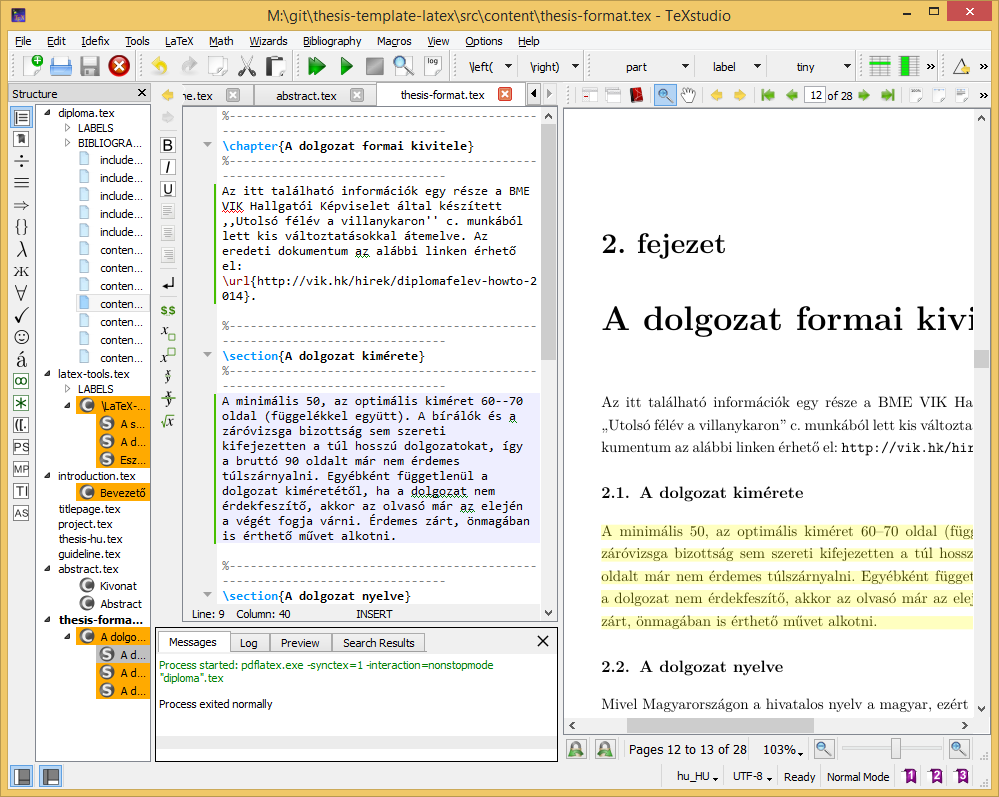
\includegraphics[width=67mm, keepaspectratio]{figures/TeXstudio.png}\hspace{1cm}
	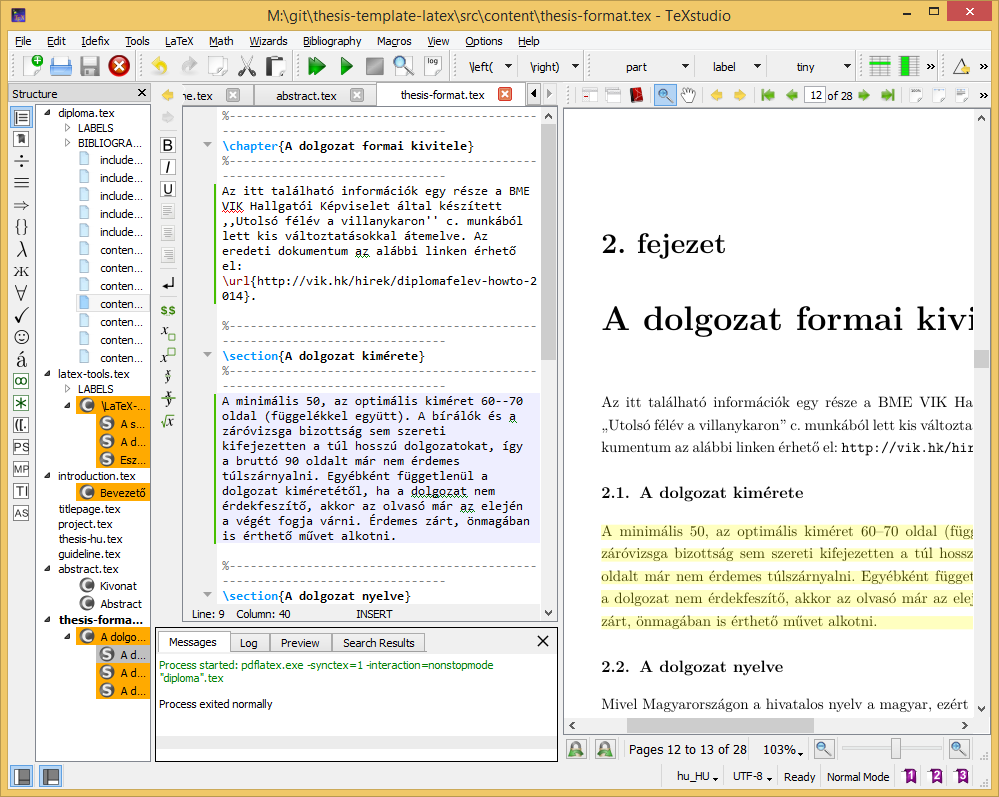
\includegraphics[width=67mm, keepaspectratio]{figures/TeXstudio.png}\\\vspace{5mm}
	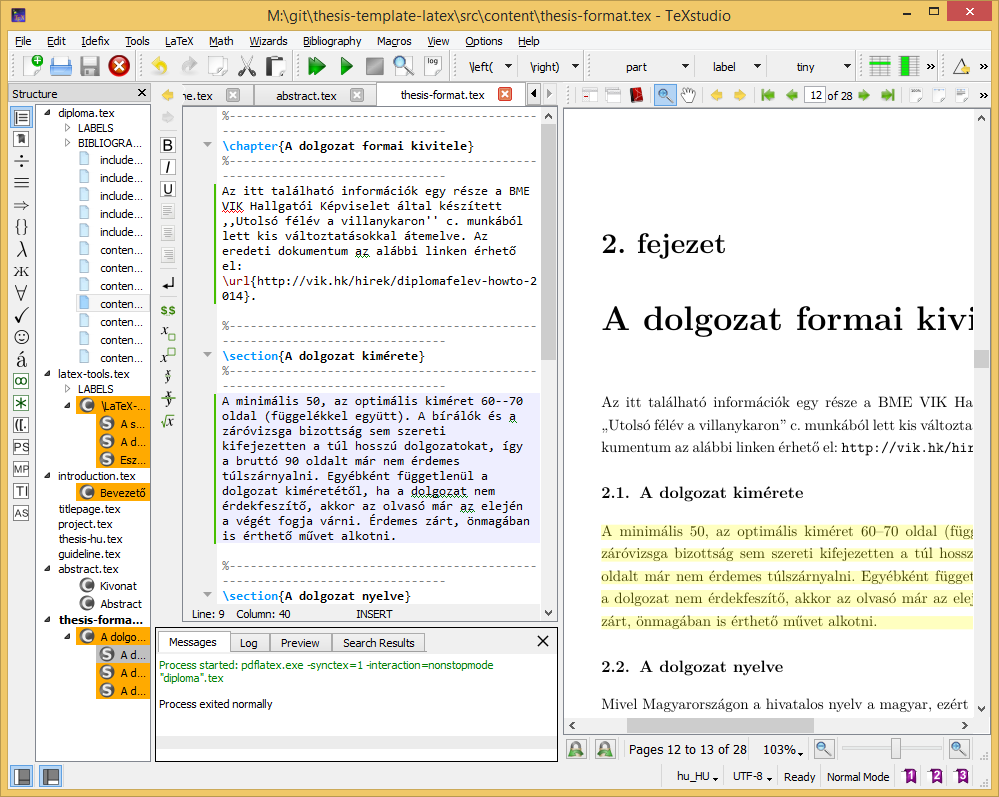
\includegraphics[width=67mm, keepaspectratio]{figures/TeXstudio.png}\hspace{1cm}
	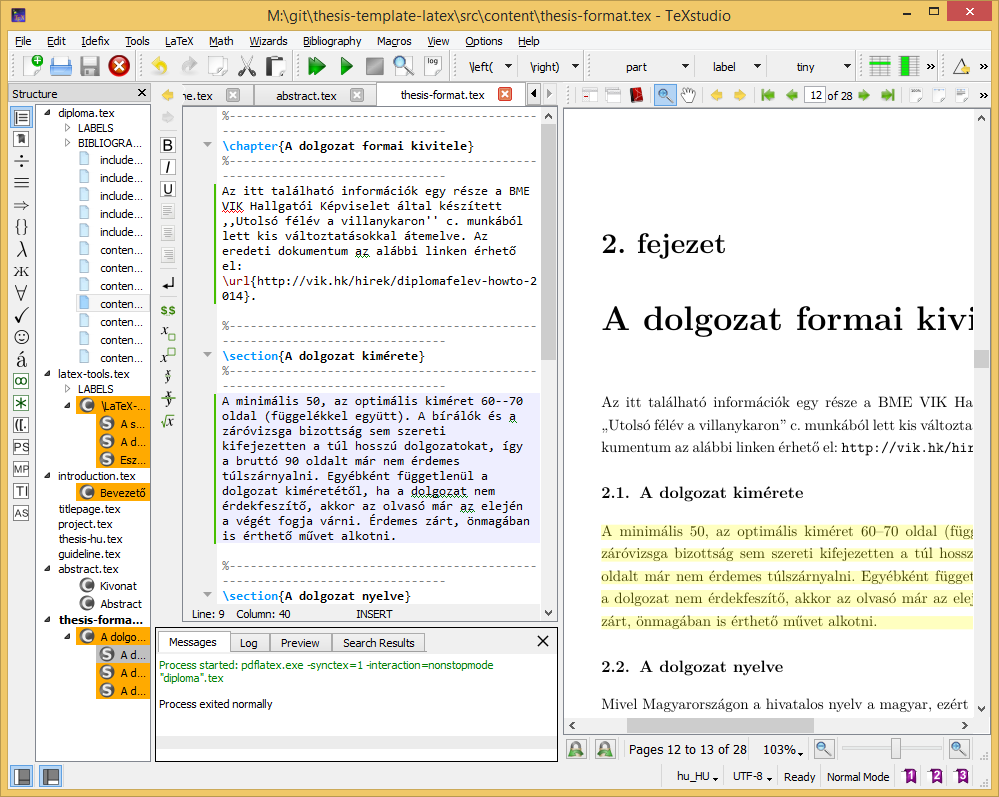
\includegraphics[width=67mm, keepaspectratio]{figures/TeXstudio.png}
	\caption{Több képfájl beillesztése esetén térközöket is érdemes használni.}
	\label{fig:HVSpaces}
\end{figure}

A táblázatok használatára \aref{tab:TabularExample}~táblázat mutat példát. A táblázatok formázásához hasznos tanácsokat találunk a \verb+booktabs+ csomag dokumentációjában.

\begin{table}[ht]
	\footnotesize
	\centering
	\begin{tabular}{ l c c }
		\toprule
		Órajel & Frekvencia & Cél pin \\
		\midrule
		CLKA & 100 MHz & FPGA CLK0\\
		CLKB & 48 MHz  & FPGA CLK1\\
		CLKC & 20 MHz  & Processzor\\
		CLKD & 25 MHz  & Ethernet chip \\
		CLKE & 72 MHz  & FPGA CLK2\\
		XBUF & 20 MHz  & FPGA CLK3\\
		\bottomrule
	\end{tabular}
	\caption{Az órajel-generátor chip órajel-kimenetei.}
	\label{tab:TabularExample}
\end{table}


%----------------------------------------------------------------------------
\section{Felsorolások és listák}
%----------------------------------------------------------------------------
Számozatlan felsorolásra mutat példát a jelenlegi bekezdés:
\begin{itemize}
	\item \emph{első bajusz:} ide lehetne írni az első elem kifejését,
	\item \emph{második bajusz:} ide lehetne írni a második elem kifejését,
	\item \emph{ez meg egy szakáll:} ide lehetne írni a harmadik elem kifejését.
\end{itemize}

Számozott felsorolást is készíthetünk az alábbi módon:
\begin{enumerate}
	\item \emph{első bajusz:} ide lehetne írni az első elem kifejését, és ez a kifejtés így néz ki, ha több sorosra sikeredik,
	\item \emph{második bajusz:} ide lehetne írni a második elem kifejését,
	\item \emph{ez meg egy szakáll:} ide lehetne írni a harmadik elem kifejését.
\end{enumerate}
A felsorolásokban sorok végén vessző, az utolsó sor végén pedig pont a szokásos írásjel. Ez alól kivételt képezhet, ha az egyes elemek több teljes mondatot tartalmaznak.

Listákban a dolgozat szövegétől elkülönítendő kódrészleteket, programsorokat, pszeudo-kódokat jeleníthetünk meg (\ref{lst:Example}.~kódrészlet).
\begin{lstlisting}[language=tex,caption=A fenti számozott felsorolás \LaTeX-forráskódja,label=lst:Example]
\begin{enumerate}
	\item \emph{els(*@ő@*) bajusz:} ide lehetne írni az els(*@ő@*) elem kifejését,
	és ez a kifejtés így néz ki, ha több sorosra sikeredik,
	\item \emph{második bajusz:} ide lehetne írni a második elem kifejését,
	\item \emph{ez meg egy szakáll:} ide lehetne írni a harmadik elem kifejését.
\end{enumerate}
\end{lstlisting}
A lista keretét, háttérszínét, egész stílusát megválaszthatjuk. Ráadásul különféle programnyelveket és a nyelveken belül kulcsszavakat is definiálhatunk, ha szükséges. Erről bővebbet a \verb+listings+ csomag hivatalos leírásában találhatunk.

%----------------------------------------------------------------------------
\section{Képletek}
%----------------------------------------------------------------------------
Ha egy formula nem túlságosan hosszú, és nem akarjuk hivatkozni a szövegből, mint például a $e^{i\pi}+1=0$ képlet, \emph{szövegközi képletként} szokás leírni. Csak, hogy másik példát is lássunk, az $U_i=-d\Phi/dt$ Faraday-törvény a $\rot E=-\frac{dB}{dt}$ differenciális alakban adott Maxwell-egyenlet felületre vett integráljából vezethető le. Látható, hogy a \LaTeX-fordító a sorközöket betartja, így a szöveg szedése esztétikus marad szövegközi képletek használata esetén is.

Képletek esetén az általános konvenció, hogy a kisbetűk skalárt, a kis félkövér betűk ($\mathbf{v}$) oszlopvektort -- és ennek megfelelően $\mathbf{v}^T$ sorvektort -- a kapitális félkövér betűk ($\mathbf{V}$) mátrixot jelölnek. Ha ettől el szeretnénk térni, akkor az alkalmazni kívánt jelölésmódot célszerű külön alfejezetben definiálni. Ennek megfelelően, amennyiben $\mathbf{y}$ jelöli a mérések vektorát, $\mathbf{\vartheta}$ a paraméterek vektorát és $\hat{\mathbf{y}}=\mathbf{X}\vartheta$ a paraméterekben lineáris modellt, akkor a \emph{Least-Squares} értelemben optimális paraméterbecslő $\hat{\mathbf{\vartheta}}_{LS}=(\mathbf{X}^T\mathbf{X})^{-1}\mathbf{X}^T\mathbf{y}$ lesz.

Emellett kiemelt, sorszámozott képleteket is megadhatunk, ennél az \verb+equation+ és a \verb+eqnarray+ környezetek helyett a korszerűbb \verb+align+ környezet alkalmazását javasoljuk (több okból, különféle problémák elkerülése végett, amelyekre most nem térünk ki). Tehát
\begin{align}
\dot{\mathbf{x}}&=\mathbf{A}\mathbf{x}+\mathbf{B}\mathbf{u},\\
\mathbf{y}&=\mathbf{C}\mathbf{x},
\end{align}
ahol $\mathbf{x}$ az állapotvektor, $\mathbf{y}$ a mérések vektora és $\mathbf{A}$, $\mathbf{B}$ és $\mathbf{C}$ a rendszert leíró paramétermátrixok. Figyeljük meg, hogy a két egyenletben az egyenlőségjelek egymáshoz igazítva jelennek meg, mivel a mindkettőt az \& karakter előzi meg a kódban. Lehetőség van számozatlan kiemelt képlet használatára is, például
\begin{align}
\dot{\mathbf{x}}&=\mathbf{A}\mathbf{x}+\mathbf{B}\mathbf{u},\nonumber\\
\mathbf{y}&=\mathbf{C}\mathbf{x}\nonumber.
\end{align}
Mátrixok felírására az $\mathbf{A}\mathbf{x}=\mathbf{b}$ inhomogén lineáris egyenlet részletes kifejtésével mutatunk példát:
\begin{align}
\begin{bmatrix}
a_{11} & a_{12} & \dots & a_{1n}\\
a_{21} & a_{22} & \dots & a_{2n}\\
\vdots & \vdots & \ddots & \vdots\\
a_{m1} & a_{m2} & \dots & a_{mn}
\end{bmatrix}
\begin{pmatrix}x_1\\x_2\\\vdots\\x_n\end{pmatrix}=
\begin{pmatrix}b_1\\b_2\\\vdots\\b_m\end{pmatrix}.
\end{align}
A \verb+\frac+ utasítás hatékonyságát egy általános másodfokú tag átviteli függvényén keresztül mutatjuk be, azaz
\begin{align}
W(s)=\frac{A}{1+2T\xi s+s^2T^2}.
\end{align}
A matematikai mód minden szimbólumának és képességének a bemutatására természetesen itt nincs lehetőség, de gyors referenciaként hatékonyan használhatók a következő linkek:\\
\indent\url{http://www.artofproblemsolving.com/LaTeX/AoPS_L_GuideSym.php},\\
\indent\url{http://www.ctan.org/tex-archive/info/symbols/comprehensive/symbols-a4.pdf},\\
\indent\url{ftp://ftp.ams.org/pub/tex/doc/amsmath/short-math-guide.pdf}.\\
Ez pedig itt egy magyarázat, hogy miért érdemes \verb+align+ környezetet használni:\\
\indent\url{http://texblog.net/latex-archive/maths/eqnarray-align-environment/}.

%----------------------------------------------------------------------------
\section{Irodalmi hivatkozások}
\label{sec:HowtoReference}
%----------------------------------------------------------------------------
Egy \LaTeX~dokumentumban az irodalmi hivatkozások definíciójának két módja van. Az egyik a \verb+\thebibliograhy+ környezet használata a dokumentum végén, az \verb+\end{document}+ lezárás előtt.
\begin{lstlisting}[language=tex]
\begin{thebibliography}{9}

\bibitem{Lamport94} Leslie Lamport, \emph{\LaTeX: A Document Preparation System}.
Addison Wesley, Massachusetts, 2nd Edition, 1994.

\end{thebibliography}
\end{lstlisting}

Ezek után a dokumentumban a \verb+\cite{Lamport94}+ utasítással hivatkozhatunk a forrásra. A fenti megadás viszonylag kötetlen, a szerző maga formázza az irodalomjegyzéket (ami gyakran inkonzisztens eredményhez vezet).

Egy sokkal professzionálisabb módszer a BiB\TeX{} használata, ezért ez a sablon is ezt támogatja. Ebben az esetben egy külön szöveges adatbázisban definiáljuk a forrásmunkákat, és egy külön stílusfájl határozza meg az irodalomjegyzék kinézetét. Ez, összhangban azzal, hogy külön formátumkonvenció határozza meg a folyóirat-, a könyv-, a konferenciacikk- stb. hivatkozások kinézetét az irodalomjegyzékben (a sablon használata esetén ezzel nem is kell foglalkoznia a hallgatónak, de az eredményt célszerű ellenőrizni). felhasznált hivatkozások adatbázisa egy \verb+.bib+ kiterjesztésű szöveges fájl, amelynek szerkezetét a \Aref{lst:Bibtex} kódrészlet demonstrálja. A forrásmunkák bevitelekor a sor végi vesszők külön figyelmet igényelnek, mert hiányuk a BiB\TeX-fordító hibaüzenetét eredményezi. A forrásmunkákat típus szerinti kulcsszó vezeti be (\verb+@book+ könyv, \verb+@inproceedings+ konferenciakiadványban megjelent cikk, \verb+@article+ folyóiratban megjelent cikk, \verb+@techreport+ valamelyik egyetem gondozásában megjelent műszaki tanulmány, \verb+@manual+ műszaki dokumentáció esetén stb.). Nemcsak a megjelenés stílusa, de a kötelezően megadandó mezők is típusról-típusra változnak. Egy jól használható referencia a \url{http://en.wikipedia.org/wiki/BibTeX} oldalon található.

\begin{lstlisting}[caption=Példa szöveges irodalomjegyzék-adatbázisra Bib\TeX{} használata esetén.,label=lst:Bibtex]
@book{Wettl04,
  author    = {Ferenc Wettl and Gyula Mayer and Péter Szabó},
  publisher = {Panem Könyvkiadó},
  title     = {\LaTeX~kézikönyv},
  year      = {2004},
}

@article{Candy86,
  author       = {James C. Candy},
  journaltitle = {{IEEE} Trans.\ on Communications},
  month        = {01},
  note         = {\doi{10.1109/TCOM.1986.1096432}},
  number       = {1},
  pages        = {72--76},
  title        = {Decimation for Sigma Delta Modulation},
  volume       = {34},
  year         = {1986},
}

@inproceedings{Lee87,
  author    = {Wai L. Lee and Charles G. Sodini},
  booktitle = {Proc.\ of the IEEE International Symposium on Circuits and Systems},
  location  = {Philadelphia, PA, USA},
  month     = {05~4--7},
  pages     = {459--462},
  title     = {A Topology for Higher Order Interpolative Coders},
  vol       = {2},
  year      = {1987},
}

@thesis{KissPhD,
  author      = {Peter Kiss},
  institution = {Technical University of Timi\c{s}oara, Romania},
  month       = {04},
  title       = {Adaptive Digital Compensation of Analog Circuit Imperfections for Cascaded Delta-Sigma Analog-to-Digital Converters},
  type        = {phdthesis},
  year        = {2000},
}

@manual{Schreier00,
  author       = {Richard Schreier},
  month        = {01},
  note         = {\url{http://www.mathworks.com/matlabcentral/fileexchange/}},
  organization = {Oregon State University},
  title        = {The Delta-Sigma Toolbox v5.2},
  year         = {2000},
}

@misc{DipPortal,
  author       = {{Budapesti Műszaki és Gazdaságtudományi Egyetem Villamosmérnöki és Informatikai Kar}},
  howpublished = {\url{http://diplomaterv.vik.bme.hu/}},
  title        = {Diplomaterv portál (2011. február 26.)},
}

@incollection{Mkrtychev:1997,
  author    = {Mkrtychev, Alexey},
  booktitle = {Logical Foundations of Computer Science},
  doi       = {10.1007/3-540-63045-7_27},
  editor    = {Adian, Sergei and Nerode, Anil},
  isbn      = {978-3-540-63045-6},
  pages     = {266-275},
  publisher = {Springer Berlin Heidelberg},
  series    = {Lecture Notes in Computer Science},
  title     = {Models for the logic of proofs},
  url       = {http://dx.doi.org/10.1007/3-540-63045-7_27},
  volume    = {1234},
  year      = {1997},
}
\end{lstlisting}

A stílusfájl egy \verb+.sty+ kiterjesztésű fájl, de ezzel lényegében nem kell foglalkozni, mert vannak beépített stílusok, amelyek jól használhatók. Ez a sablon a BiB\TeX-et használja, a hozzá tartozó adatbázisfájl a \verb+mybib.bib+ fájl. Megfigyelhető, hogy az irodalomjegyzéket a dokumentum végére (a \verb+\end{document}+ utasítás elé) beillesztett \verb+\bibliography{mybib}+ utasítással hozhatjuk létre, a stílusát pedig ugyanitt a  \verb+\bibliographystyle{plain}+ utasítással adhatjuk meg. Ebben az esetben a \verb+plain+ előre definiált stílust használjuk (a sablonban is ezt állítottuk be). A \verb+plain+ stíluson kívül természetesen számtalan más előre definiált stílus is létezik. Mivel a \verb+.bib+ adatbázisban ezeket megadtuk, a BiB\TeX-fordító is meg tudja különböztetni a szerzőt a címtől és a kiadótól, és ez alapján automatikusan generálódik az irodalomjegyzék a stílusfájl által meghatározott stílusban.

Az egyes forrásmunkákra a szövegből továbbra is a \verb+\cite+ paranccsal tudunk hivatkozni, így \aref{lst:Bibtex}.~kódrészlet esetén a hivatkozások rendre \verb+\cite{Wettl04}+, \verb+\cite{Candy86}+, \verb+\cite{Lee87}+, \verb+\cite{KissPhD}+, \verb+\cite{Schreirer00}+,
\verb+\cite{Mkrtychev:1997}+ és \verb+\cite{DipPortal}+. Az egyes forrásmunkák sorszáma az irodalomjegyzék bővítésekor változhat. Amennyiben az aktuális számhoz illeszkedő névelőt szeretnénk használni, használjuk az \verb+\acite{}+ parancsot.

Az irodalomjegyzékben alapértelmezésben csak azok a forrásmunkák jelennek meg, amelyekre található hivatkozás a szövegben, és ez így alapvetően helyes is, hiszen olyan forrásmunkákat nem illik az irodalomjegyzékbe írni, amelyekre nincs hivatkozás.

Mivel a fordítási folyamat során több lépésben oldódnak fel a szimbólumok, ezért gyakran többször is le kell fordítani a dokumentumot. Ilyenkor ez első 1-2 fordítás esetleg szimbólum-feloldásra vonatkozó figyelmeztető üzenettel zárul. Ha hibaüzenettel zárul bármelyik fordítás, akkor nincs értelme megismételni, hanem a hibát kell megkeresni. A \verb+.bib+ fájl megváltoztatáskor sokszor nincs hatása a változtatásnak azonnal, mivel nem mindig fut újra a BibTeX fordító. Ezért célszerű a változtatás után azt manuálisan is lefuttatni (TeXstudio esetén \verb+Tools/Bibliography+).

Hogy a szövegbe ágyazott hivatkozások kinézetét demonstráljuk, itt most sorban meghivatkozzuk a \cite{Wettl04}, \cite{Candy86}, \cite{Lee87}, \cite{KissPhD}, \cite{Schreier00} és \acite{Mkrtychev:1997}\footnote{Informatikai témában gyakran hivatkozunk cikkeket a Springer LNCS valamely kötetéből, ez a hivatkozás erre mutat egy helyes példát.} forrásmunkát, valamint \acite{DipPortal} weboldalt.

Megjegyzendő, hogy az ékezetes magyar betűket is tartalmazó \verb+.bib+ fájl az \verb+inputenc+ csomaggal betöltött \verb+latin2+ betűkészlet miatt fordítható. Ugyanez a \verb+.bib+ fájl hibaüzenettel fordul egy olyan dokumentumban, ami nem tartalmazza a \verb+\usepackage[latin2]{inputenc}+ sort. Speciális igény esetén az irodalmi adatbázis általánosabb érvényűvé tehető, ha az ékezetes betűket speciális latex karakterekkel helyettesítjük a \verb+.bib+ fájlban, pl. á helyett \verb+\'{a}+-t vagy ő helyett \verb+\H{o}+-t írunk.

Irodalomhivatkozásokat célszerű először olyan szolgáltatásokban keresni, ahol jó minőségű bejegyzések találhatók (pl. ACM Digital Library,\footnote{\url{https://dl.acm.org/}} DBLP,\footnote{\url{http://dblp.uni-trier.de/}} IEEE Xplore,\footnote{\url{http://ieeexplore.ieee.org/}} SpringerLink\footnote{\url{https://link.springer.com/}}) és csak ezek után használni kevésbé válogatott forrásokat (pl. Google Scholar\footnote{\url{http://scholar.google.com/}}). A jó minőségű bejegyzéseket is érdemes megfelelően tisztítani.\footnote{\url{https://github.com/FTSRG/cheat-sheets/wiki/BibTeX-Fixing-entries-from-common-sources}} A sablon angol nyelvű változatában használt \texttt{plainnat} beállítás egyik sajátossága, hogy a cikkhez generált hivatkozás a cikk DOI-ját és URL-jét is tartalmazza, ami gyakran duplikátumhoz vezet -- érdemes tehát a DOI-kat tartalmazó URL mezőket törölni. 

%----------------------------------------------------------------------------
\section{A dolgozat szerkezete és a forrásfájlok}
%----------------------------------------------------------------------------
A diplomatervsablonban a TeX fájlok két alkönyvtárban helyezkednek el. Az \verb+include+ könyvtárban azok szerepelnek, amiket tipikusan nem kell szerkesztenünk, ezek a sablon részei (pl. címoldal). A \verb+content+ alkönyvtárban pedig a saját munkánkat helyezhetjük el. Itt érdemes az egyes fejezeteket külön \TeX{} állományokba rakni.

A diplomatervsablon (a kari irányelvek szerint) az alábbi fő fejezetekből áll:
\begin{enumerate}
	\item 1 oldalas \emph{tájékoztató} a szakdolgozat/diplomaterv szerkezetéről (\verb+include/guideline.tex+), ami a végső dolgozatból törlendő,
	\item \emph{feladatkiírás} (\verb+include/project.tex+), a dolgozat nyomtatott verzójában ennek a helyére kerül a tanszék által kiadott, a tanszékvezető által aláírt feladatkiírás, a dolgozat elektronikus verziójába pedig a feladatkiírás egyáltalán ne kerüljön bele, azt külön tölti fel a tanszék a diplomaterv-honlapra,
	\item \emph{címoldal} (\verb+include/titlepage.tex+),
	\item \emph{tartalomjegyzék} (\verb+thesis.tex+),
	\item a diplomatervező \emph{nyilatkozat}a az önálló munkáról (\verb+include/declaration.tex+),
	\item 1-2 oldalas tartalmi \emph{összefoglaló} magyarul és angolul, illetve elkészíthető még további nyelveken is (\verb+content/abstract.tex+),
	\item \emph{bevezetés}: a feladat értelmezése, a tervezés célja, a feladat indokoltsága, a diplomaterv felépítésének rövid összefoglalása (\verb+content/introduction.tex+),
	\item sorszámmal ellátott \emph{fejezetek}: a feladatkiírás pontosítása és részletes elemzése, előzmények (irodalomkutatás, hasonló alkotások), az ezekből levonható következtetések, a tervezés részletes leírása, a döntési lehetőségek értékelése és a választott megoldások indoklása, a megtervezett műszaki alkotás értékelése, kritikai elemzése, továbbfejlesztési lehetőségek,
	\item esetleges \emph{köszönetnyilvánítás}ok (\verb+content/acknowledgement.tex+),
	\item részletes és pontos \emph{irodalomjegyzék} (ez a sablon esetében automatikusan generálódik a \verb+thesis.tex+ fájlban elhelyezett \verb+\bibliography+ utasítás hatására, \az+\refstruc{sec:HowtoReference}ban leírtak szerint),
	\item \emph{függelékek} (\verb+content/appendices.tex+).
\end{enumerate}

A sablonban a fejezetek a \verb+thesis.tex+ fájlba vannak beillesztve \verb+\include+ utasítások segítségével. Lehetőség van arra, hogy csak az éppen szerkesztés alatt álló \verb+.tex+ fájlt fordítsuk le, ezzel lerövidítve a fordítási folyamatot. Ezt a lehetőséget az alábbi kódrészlet biztosítja a \verb+thesis.tex+ fájlban.
\begin{lstlisting}
\includeonly{
	guideline,%
	project,%
	titlepage,%
	declaration,%
	abstract,%
	introduction,%
	chapter1,%
	chapter2,%
	chapter3,%
	acknowledgement,%
	appendices,%
}
\end{lstlisting}

Ha az alábbi kódrészletben az egyes sorokat a \verb+%+ szimbólummal kikommentezzük, akkor a megfelelő \verb+.tex+ fájl nem fordul le. Az oldalszámok és a tartalomjegyék természetesen csak akkor billennek helyre, ha a teljes dokumentumot lefordítjuk.

%----------------------------------------------------------------------------
\newpage
\section{Alapadatok megadása}
%----------------------------------------------------------------------------
A diplomaterv alapadatait (cím, szerző, konzulens, konzulens titulusa) a \verb+thesis.tex+ fájlban lehet megadni.

%----------------------------------------------------------------------------
\section{Új fejezet írása}
%----------------------------------------------------------------------------
A főfejezetek külön \verb+content+ könyvtárban foglalnak helyet. A sablonhoz 3 fejezet készült. További főfejezeteket úgy hozhatunk létre, ha új \TeX~fájlt készítünk a fejezet számára, és a \verb+thesis.tex+ fájlban, a \verb+\include+ és \verb+\includeonly+ utasítások argumentumába felvesszük az új \verb+.tex+ fájl nevét.


%----------------------------------------------------------------------------
\section{Definíciók, tételek, példák}
%----------------------------------------------------------------------------

\begin{definition}[Fluxuskondenzátor térerőssége]
Lorem ipsum dolor sit amet, consectetur adipiscing elit, sed do eiusmod tempor incididunt ut labore et dolore magna aliqua. Ut enim ad minim veniam, quis nostrud exercitation ullamco laboris nisi ut aliquip ex ea commodo consequat.
\end{definition}

\begin{example}
Példa egy példára. Duis aute irure dolor in reprehenderit in voluptate velit esse cillum dolore eu fugiat nulla pariatur. Excepteur sint occaecat cupidatat non proident, sunt in culpa qui officia deserunt mollit anim id est laborum.
\end{example}

\begin{theorem}[Kovács tétele]
Duis aute irure dolor in reprehenderit in voluptate velit esse cillum dolore eu fugiat nulla pariatur. Excepteur sint occaecat cupidatat non proident, sunt in culpa qui officia deserunt mollit anim id est laborum.
\end{theorem}

\chapter{Bevezetés}
Napjainkban egyre több fizikai eszközt váltanak fel pluginok a zeneiparban. Már jelenleg is 
meghatározó részei stúdióknak, professzionális és hobbi zenészek is előszeretettel használják 
ezeket.

A digitális pluginok fontossága a zeneiparban az elmúlt évtizedekben drámaian megnövekedett, ahogy 
a technológia fejlődött és a digitális munkafolyamatok egyre inkább előtérbe kerültek. A pluginok 
olyan szoftveres eszközök, amelyek digitális audio munkaállomásokban (DAW-okban) működnek, és 
különféle zenei és hangfeldolgozási funkciókat látnak el.

\section{A feladat megfogalmazása}
A feladatom az Orange Crush 20L gitárerősítő digitális modellezése, és ezalapján elkészíteni egy 
VST3 plugint, ami valós időben futtatható. Cél, hogy a plugin által biztosított hangzás megegyezzen 
az erősítőjével, és helyettesíteni tudja azt.
\chapter{Analóg áramkörök digitális modellezése}

\section{Lineáris áramkörök modellezése}

A lineáris áramkörök modellezésének a leggyakoribb módszereit említem meg~\cite{transformations}~\cite{eulers}.

Egy lineáris, idő-invariáns rendszert pontosan jellemez az átviteli függvénye, aminek a definíciója  a kimenet 
Laplace-transzformáltjának és a bemenet Laplace-transzformáltjának hányadosa.
\begin{equation}
    H(s)=\frac{Y(s)}{U(s)}
\end{equation}
Ennek a videlkedésnek a megvalósítása a cél diszkrét időben.

Lehetséges az a megközelítés is, hogy az állapotváltozós leírás alapján kifejezett rendszert szimulálunk. Ekkor minden belső változó is számolható lenne, de a leggyakoribb esetekben erre nincs szükség, és csak a rendszer kimenete lényeges. Az állapotváltozós leírás alapján való szimuláció több egyenlet megoldását igényelné, így a minél kisebb számítási igény céljából lineáris hálózat esetén kerülendő.

Az összes alább mutatott diszkretizálási módszerek alkalmazásakor behelyettesítés után az átviteli függvény az alábbi alakot veszi fel:
\begin{equation}
    \frac{Y(z)}{U(z)}=\frac{\sum_{i=0}^{N}b_i z^{-i}}{1+\sum_{j=1}^{M}a_j z^{-j}}
\end{equation}
Ezt az egyenletet átrendezve:
\begin{equation}
    Y(z)(1+\sum_{j=1}^{M}a_j z^{-j})=U(z)\sum_{i=0}^{N}b_i z^{-i}
\end{equation}
\begin{equation}
    Y(z)+\sum_{j=1}^{M}a_j Y(z)z^{-j}=\sum_{i=0}^{N}b_i U(z)z^{-i}
\end{equation}
\begin{equation}
    Y(z)=\sum_{j=1}^{M}-a_j Y(z)z^{-j}+\sum_{i=0}^{N}b_i U(z)z^{-i}
\end{equation}
Inverz z-transzormálva megkapjuk a rendszeregyenletet:
\begin{equation}
    y[n]=\sum_{j=1}^{M}-a_j y[n-j]+\sum_{i=0}^{N}b_i u[n-i]
\end{equation}

A szimuláció során ezt az egyenletet kell leprogramozni, ahol az $y$ változónak (válasz) az utolsó $M$ értékét, az $u$ változónak (gerjesztés) pedig az utolsó $N$ értékét kell eltárolnunk a válasz következő értékének számolásához. A bufferelést érdemes cirkuláris bufferrel megvalósítani a számítási igény csökkentésének érdekében. 

\subsection{Előrelépő Euler-módszer}\label{fwEulerSection}

Az előrelépő (explicit) Euler-módszer a deriváltat a következő és az aktuális állapotváltozóból fejezi ki, a többi tagnak
az ezelőtti állapotát használja.
\begin{equation}
    \mathbf{\dot{w}}=\frac{\mathbf{w}[n+1]-\mathbf{w}[n]}{\Delta{}t}
\label{fwEuler}
\end{equation}
\begin{equation}
    \mathbf{\dot{w}}=\frac{\mathbf{w}[n+1]-\mathbf{w}[n]}{\Delta{}t}=\mathbf{A}\mathbf{w}[n]+\mathbf{Bu}[n]
\end{equation}
Az $s$-re kifejezve~\ref{fwEuler} alapján:
\begin{equation}
    s=\frac{z-1}{T}=\frac{1-z^{-1}}{Tz^{-1}}
\label{fwEulers}
\end{equation}

Az előrelépő Euler-módszer nem mindig fog stabil folytonos idejű rendszerből stabil diszkrét idejű rendszert 
eredményezni, ami~\ref{fwEulers}-ből egyértelműen kifejezhető~\cite{transformations}. A stabilitás függeni fog a mintavételi frekvenciától, és ha az nem elég nagy, akkor instabil lesz a diszkretizált rendszer.
\begin{equation}
    z=sT+1
\end{equation}

\begin{figure}[!h]
    \centering
    \begin{subfigure}{0.47\textwidth}
        \centering
        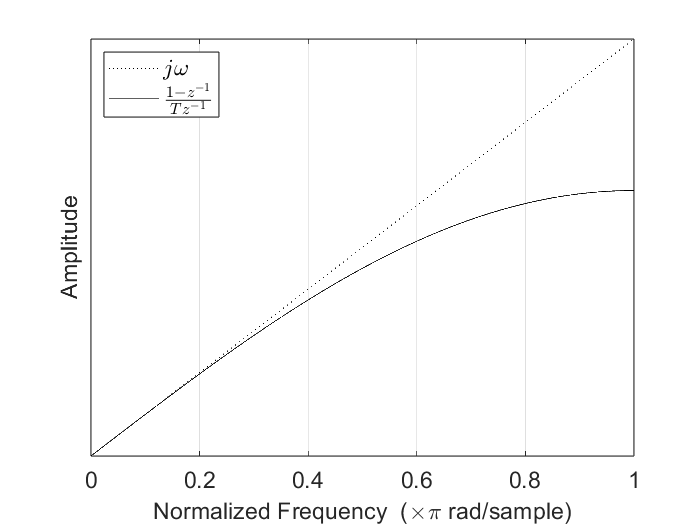
\includegraphics[scale=0.38]{figures/fwEulerA.png}
        \caption{}
    \end{subfigure}
    \hfill
    \begin{subfigure}{0.47\textwidth}
        \centering
        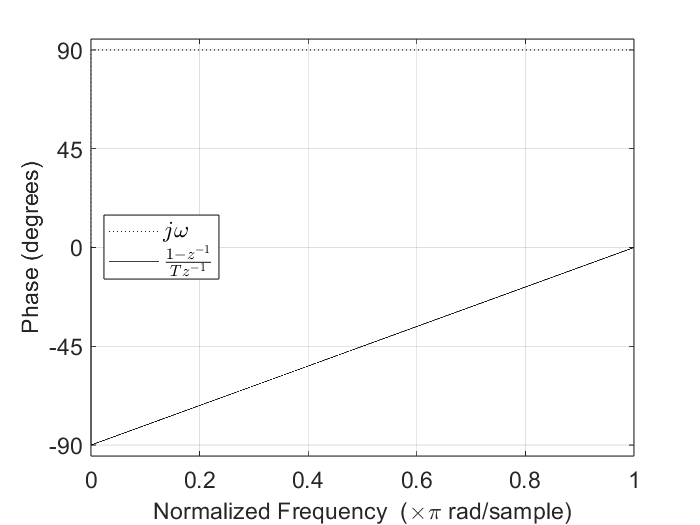
\includegraphics[scale=0.38]{figures/fwEulerP.png}
        \caption{}
    \end{subfigure}
    \caption{Az előrelépő Euler-módszer frekvenciatorzítása}
\end{figure}

\begin{figure}[H]
    \centering
    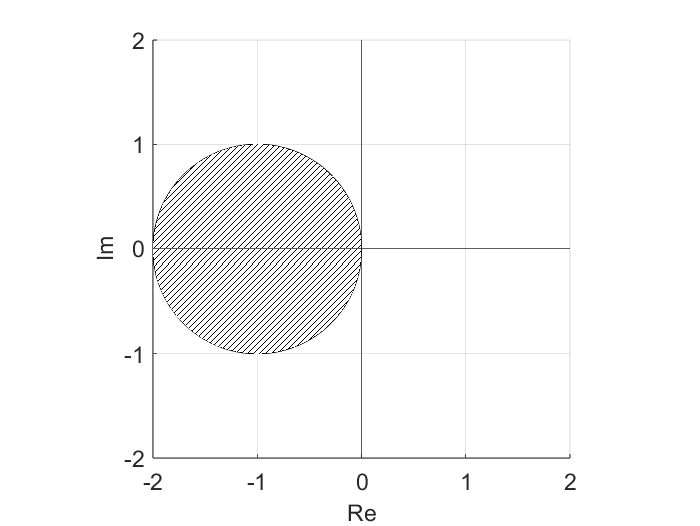
\includegraphics[scale=0.5]{figures/fwEulerS.png}
    \caption{Az előrelépő Euler-módszer alkalmazásával létrehozott diszkrét rendszer stabilitásának feltétele: az $sT$ szorzatnak az ábrán jelölt tartományom belül kell lennie}
\end{figure}

\subsection{Hátralépő Euler-módszer}\label{bwEulerSection}

A hátralépő (implicit) Euler-módszer a deriváltat az aktuális és az ezelőtti állapotváltozóból fejezi ki, a többi tagnak
az aktuális állapotát használja.
\begin{equation}
    \mathbf{\dot{w}}=\frac{\mathbf{w}[n]-\mathbf{w}[n-1]}{\Delta{}t}
\label{bwEuler}
\end{equation}
\begin{equation}
    \mathbf{\dot{w}}=\frac{\mathbf{w}[n]-\mathbf{w}[n-1]}{\Delta{}t}=\mathbf{A}\mathbf{w}[n]+\mathbf{Bu}[n]
\end{equation}
Az $s$-re kifejezve~\ref{bwEuler} alapján:
\begin{equation}
    s=\frac{1-z^{-1}}{T}=\frac{z-1}{Tz}
\label{bwEulers}
\end{equation}
A hátralépő Euler-módszerrel modellezett folytonos idejű rendszer mindig stabil diszkrét idejű rendszerhez vezet, 
ami~\ref{bwEulers} alapján belátható~\cite{transformations}.  
\begin{equation}
    z=\frac{1}{1-sT}
\end{equation}

\begin{figure}[!h]
    \centering
    \begin{subfigure}{0.47\textwidth}
        \centering
        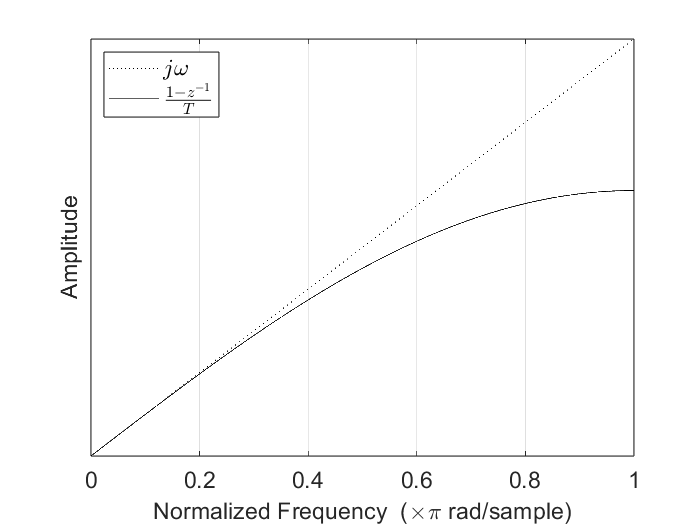
\includegraphics[scale=0.38]{figures/bwEulerA.png}
        \caption{}
    \end{subfigure}
    \hfill
    \begin{subfigure}{0.47\textwidth}
        \centering
        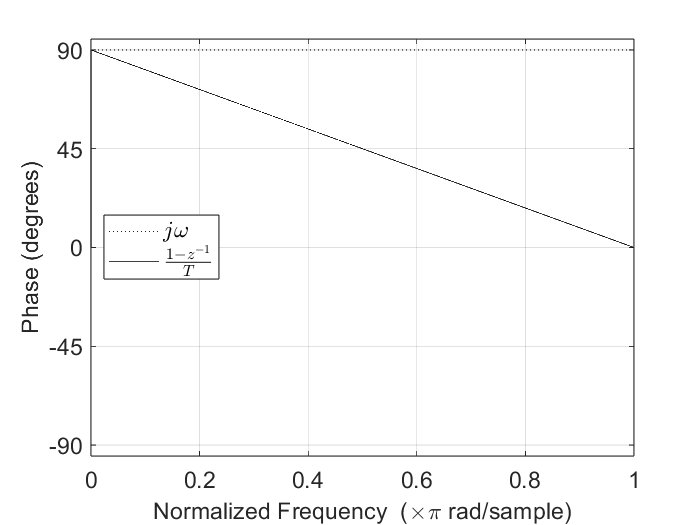
\includegraphics[scale=0.38]{figures/bwEulerP.png}
        \caption{}
    \end{subfigure}
    \caption{A hátralépő Euler-módszer frekvenciatorzítása}
\end{figure}

\begin{figure}[H]
    \centering
    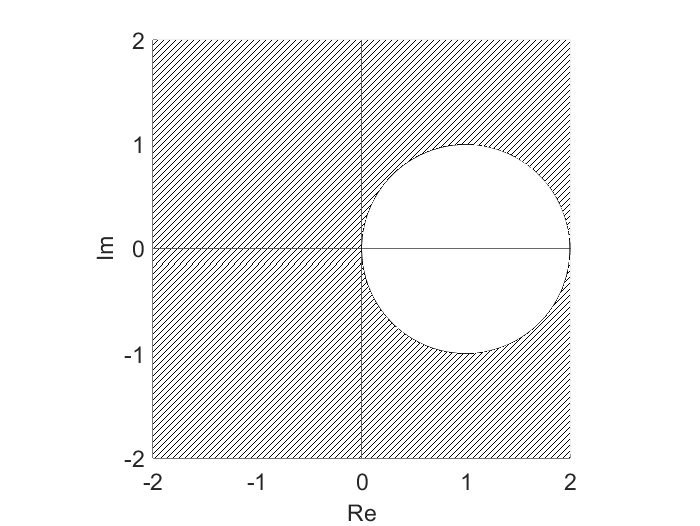
\includegraphics[scale=0.5]{figures/bwEulerS.png}
    \caption{A hátralépő Euler-módszer alkalmazásával létrehozott diszkrét rendszer stabilitásának feltétele: az $sT$ szorzatnak az ábrán jelölt tartományom belül kell lennie}
\end{figure}

\subsection{Bilineáris transzformáció}

Egyik leggyakrabban használt módszer a bilineáris transzformáció, amely az s-síkból a z-síkba transzformál a trapézszabály, azaz 
az előre- és a hátralépő Euler-módszer átlaga szerint.
\begin{equation}
    s=\frac{2}{T}\frac{z-1}{z+1}=\frac{2}{T}\frac{1-z^{-1}}{1+z^{-1}}
    \label{bilin}
\end{equation}
A transzformáció után a rendszer stabilitása megmarad, amit~\ref{bilin}-ből könnyen ki lehet fejezni~\cite{transformations}.

\begin{equation}
    z=-\frac{4}{sT-2}-1
\end{equation}

\begin{figure}[!h]
    \centering
    \begin{subfigure}{0.47\textwidth}
        \centering
        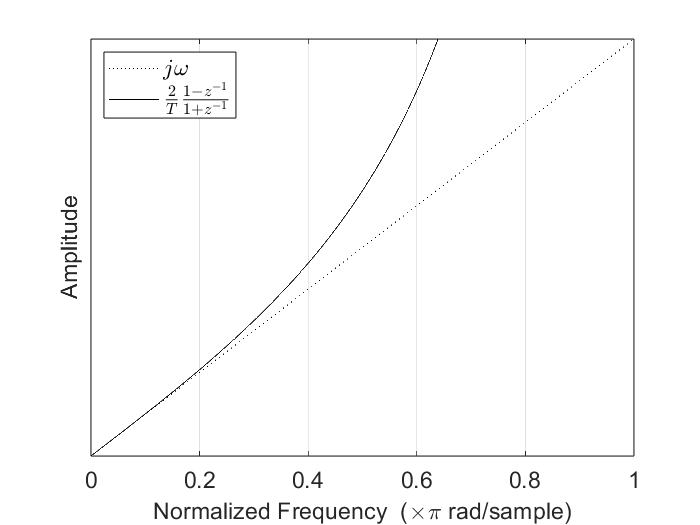
\includegraphics[scale=0.38]{figures/bilinearA.png}
        \caption{}
    \end{subfigure}
    \hfill
    \begin{subfigure}{0.47\textwidth}
        \centering
        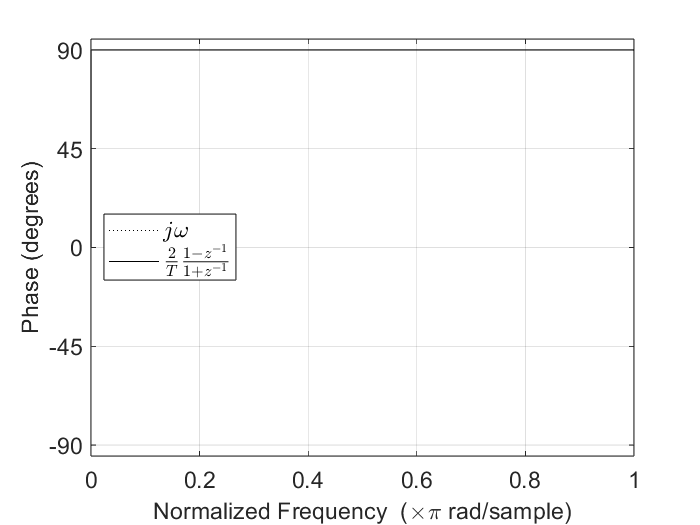
\includegraphics[scale=0.38]{figures/bilinearP.png}
        \caption{}
    \end{subfigure}
    \caption{A bilineáris transzformáció frekvenciatorzítása}
\end{figure}

\begin{figure}[H]
    \centering
    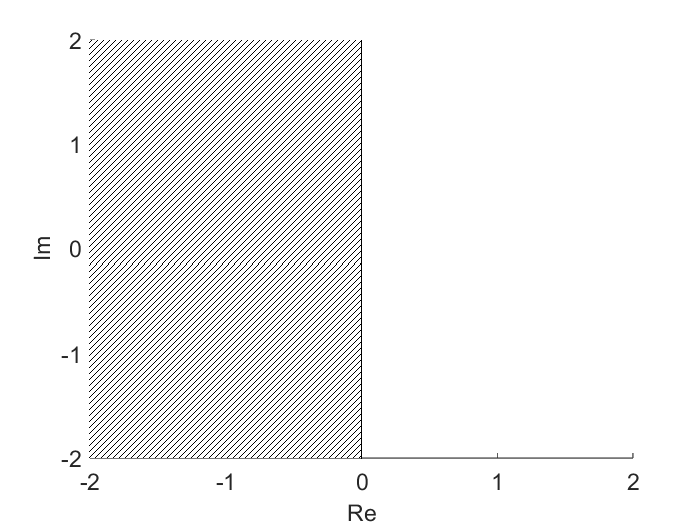
\includegraphics[scale=0.5]{figures/bilinearS.png}
    \caption{A bilineáris transzformáció alkalmazásával létrehozott diszkrét rendszer stabilitásának feltétele: az $sT$ szorzatnak az ábrán jelölt tartományom belül kell lennie}
\end{figure}
Az ábrák alapján látszólag a hátralépő Euler-módszer szerinti diszkretizálás célszerűbb, viszont ez nem így van. A bilineáris transzformációval diszkretizált megoldás pontosabb, hiszen a derivált pontosabban van közelítve (a Taylor-sorának első elemével). A végeredményben így kisebb a hiba a kimenetben, mint a hátralépő Euler-módszer szerinti diszkretizálás esetén.
\subsection{Impulzus invariáns transzformáció}

Az impulzus invariáns transzformációhoz ugyanúgy szükség van a transzformálni kívánt rendszer átviteli függvényére.
\begin{equation}
    H(s)=\frac{B(s)}{A(s)}\triangleq\frac{b_0s^{N-1}+b_1s^{N-2}+\cdots+b_{N-2}s+b_{N-1}}{s^N+a_1s^{N-1}+\cdots+a_{N-1}s+b_{N}}
\end{equation}
Az átviteli függvényt részlettörtekre bontva, inverz Laplace-transzformálva, majd mintavételezve:
\begin{equation}
    H(s)=\sum_{i=1}^{N}\frac{K_i}{s-s_i}
\end{equation}
\begin{equation}
    h(t)=\sum_{i=1}^{N}K_i e^{s_i t}
\end{equation}
\begin{equation}
    h[n]=\sum_{i=1}^{N}K_i e^{s_i nT}
\end{equation}
Ezt z-transzformálva kapjuk meg az impulzus-invariáns transzformáció segítségével megtervezett digitális 
szűrőt.
\begin{equation}
    H(z)=\sum_{i=1}^{N}\frac{K_i}{1-e^{s_i T}z^{-1}}
    \label{impinv}
\end{equation}


A transzformáció után a rendszer stabilitása megmarad, hiszen a transzformáció során $s$ és $z$ között a pontos összefüggést használjuk, és nem közelítünk~\cite{transformations}. 
\begin{equation}
    z_i\triangleq e^{s_i T}
\end{equation} 
Ennek köszönhetően frekvenciatorzítás sem lép fel a transzformáció után.




\section{Nemlineáris elemek}
Ha a rendszerbe memória nélküli nemlinearitás kerül, akkor az átviteli függvény nem értelmezett.

Az állapotváltzós leírás egy differenciálegyenlet rendszer, ami egy hálózatot pontosan meghatároz. Mivel az átviteli függvény nem értelmezett a nemlinearitás miatt, így az állapotváltozós leírás segítségével kell modellezni a hálózatot. Ekkor az állapotváltozós leírásban 
meg fog jelenni a nemlineáris függvény.
\begin{equation}
    \mathbf{\dot{w}}(t)=\mathbf{A}\mathbf{w}(t)+\mathbf{Bu}(t)+\mathbf{Cf}(\mathbf{w}(t),\mathbf{u}(t))
\end{equation}

Leggyakrabban a megoldáshoz az Euler-módszerek és a Runge-Kutta módszerek használatosak~\cite{eulers}~\cite{rungekutta}~\cite{rkk}.

\subsection{Előrelépő Euler-módszer}
Az előrelépő Euler-módszer használatánál az egyenletrendszer gyakran egyszerűen megoldható lesz, átrendezés után az előző 
állapotokat behelyettesítve kapható meg a következő állapot.

Diszkretizáláshoz a (\ref{bwEulers}) egyenletet használandó, ezt behelyettesítve, és rendezve:
\begin{equation}
    \mathbf{w}[n+1]=\mathbf{A'}\mathbf{w}[n]+\mathbf{B'u}[n]+\mathbf{C'f}(\mathbf{w}[n], \mathbf{u}[n])
\end{equation}
Ezt átrendezve:
\begin{equation}
    \mathbf{w}[n]=\mathbf{A'}\mathbf{w}[n-1]+\mathbf{B'u}[n-1]+\mathbf{C'f}(\mathbf{w}[n-1],\mathbf{u}[n-1])
\end{equation}
Az átalakítások után sok esetben csak a korábbi értékeinket be kell helyettesítenünk az explicit egyenletbe a következő minta számolásához.

Ahogy a~\ref{fwEulerSection} részben látható, lehetséges, hogy a diszkretizált rendszer instabil lesz. Ez a mintavételi frekvenciától függ, és gyakran ez nagyon nagy frekvencia esetén lesz csak stabil a rendszer. Ez a feltétel legtöbbször nem teljesíthető valós idejű szimuláció esetén, így ritkán használatos.

\subsection{Hátralépő Euler-módszer}
A hátrelépő Euler-módszer használatával új problémák merülnek fel, viszont a stabilitási kérdés megoldódik. 
Az állapotváltozós leírás transzformálása és rendezése egy implicit egyenletrendszerhez vezet.
\begin{equation}
    \mathbf{w}[n]=\mathbf{A'}\mathbf{w}[n-1]+\mathbf{B'u}[n]+\mathbf{C'f}(\mathbf{w}[n],\mathbf{u}[n])
\end{equation}
Látható, hogy az egyenletrendszer bal és jobb oldalán is (jobb oldalon a függvény argumentumaként) megtalálható az $\mathbf{w}[n]$ állapotváltozó. Az implicit egyenlet valamely zérushely-kereső algoritmussal megoldandó 
(intervallumfelezés, Newton-módszer, szelőmódszer stb.~\cite{bookNewton}). A nehézségeket pedig az ellensúlyozza, hogy az implicit egyenlet megoldásának árán stabil folytonos idejű rendszerből stabil diszkrét idejű rendszer lesz.

\subsection{Negyedfokú Runge-Kutta módszer}
A Runge-Kutta módszereket gyakran szokták használni nemlineáris rendszerek offline szimulációjánál. Alapötletük hasonló, mint az Euler-módszereknek, viszont itt több pontból közelítik a deriváltat. Így ha a az eredeti rendszernek a nagyon pontos modellezése a cél, akkor jobb eredményt biztosítanak, mint az Euler-módszerek. Viszont nagyobb a számításigényük, és nem alkalmazhatóak valós időben, hiszen a számításhoz gerjesztést szükséges olyan pontokban is ismerni, ami általában egy valós idejű alkalmaás esetén nem lehetséges. Leggyakrabban használt verziója a negyedfokú Runge-Kutta módszer (RK4)~\cite{rkk}~\cite{rungekutta}.

A negyedfokú Runge-Kutta (RK4) módszerre a matematikusok a leghatékonyabb numerikus közönséges differenciálegyenlet megoldó módszerként hivatkoznak~\cite{rk4}, mert a magasabb fokú változatok a pontosságot csak kis mértékben tudják növelni a hozzáadott nagy számítási igény mellett. A módszer alapfeltétele, hogy ismert a nemlineáris differenciálegyenlet, és a kezdeti értékek adottak:
\begin{equation}
    \begin{cases}
        \mathbf{\dot{w}}=f(\mathbf{w}(t), \mathbf{u}(t))\\
        \mathbf{w}(t_0)=\mathbf{w_0} 
    \end{cases}
\end{equation}
Ekkor legyen $h=T$, és felírható:
\begin{equation}
    \begin{cases}
        w[n+1]=w[n]+u[n]+\frac{h}{6}(K_1+2K_2+2K_3+K_4)\\
        K_1=f(w[n], u(nT))\\
        K_2=f(w[n]+h\frac{K_1}{2}, u(nT+\frac{h}{2}))\\
        K_3=f(w[n]+h\frac{K_2}{2}, u(nT+\frac{h}{2}))\\
        K_4=f(w[n]+hK_3, u(nT+h))
    \end{cases}
\end{equation}
Ebben az egyenletrendszerben:
\begin{itemize}
    \item $K_1$ a függvény meredeksége az intervallum kezdetén $y$ alapján számítva
    \item $K_2$ a függvény meredeksége a intervallum közepén $y$ és $K_1$ alapján számolva 
    \item $K_3$ a függvény meredeksége a intervallum közepén $y$ és $K_2$ alapján számolva
    \item $K_4$ a függvény meredeksége a intervallum végén $y$ és $K_3$ alapján számolva
\end{itemize}
Mint látható, $K_2$ és $K_3$ számolásához szükség lenne a gerjesztés két mintavételezési pont közötti értékére, így valós időben nem, vagy csak nehezen alkalmazható.
\chapter{K-módszer}

A K-módszer (Kirchoff-módszer) célja, hogy szétválassza a rendszer lineáris részét és az olyan 
részt, amelyben késleltetés nélküli út van. Ezután a késleltetés nélküli részt 
geometriai módszerekkel oldja meg.

\section{A K-módszer alapgondolata}\label{KSep}
A K-módszer alapfeltevése, hogy a modellezendő rendszer felbontható egy lineáris dinamikus és egy 
nemlineáris memória nélküli részre~\cite{borin}\cite{borin2}\cite{otherK}. 
\begin{equation}
    \begin{cases}
        \mathbf{x}(t)=\mathbf{L}(\mathbf{y}(t),\mathbf{u}(t)) \\
        \mathbf{y}(t)=\mathbf{f}_{NL}(\mathbf{x}(t)) 
    \end{cases} 
\end{equation}
Így, hogy a rendszer két részre van osztva, azokat a bemeneteket és kimeneteket fogják érinteni 
a számolási nehézségek, amelyek függenek a nemlineáris résztől.
\begin{figure}[H]
    \centering
    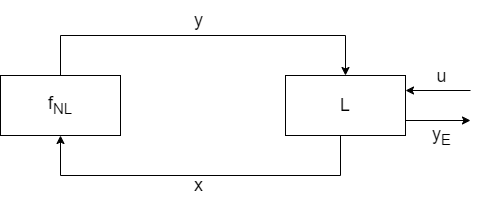
\includegraphics[scale=0.5]{figures/xy.png}
    \caption{A K-módszer alapfeltétele; $\mathbf{u}$ a bemenet, és $\mathbf{y_E}$ a kimenet a külvilág felé}
\end{figure}
Ha a rendszert a hátralépő Euler módszer, akár a bilineáris transzformáció segítségével diszkretizáljuk, akkor a következő összefüggéshez jutunk~\cite{borin}:
\begin{equation}
    \mathbf{x}[n]=\mathbf{Ky}[n]+\mathbf{p}[n]    
\end{equation}
ahol a rendszernek $M$ darab ``belső`` bemente ($y_1 \ldots y_M$), $P$ darab ``külső`` bemenete ($u_1 \ldots u_P$) és $N$ darab ``belső`` kimenete ($x_1 \ldots x_N$) van.

\begin{figure}[H]
    \centering
    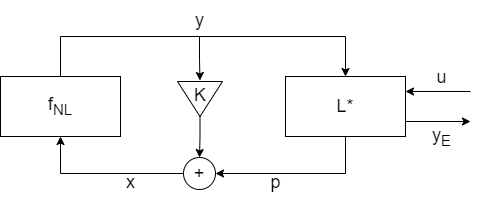
\includegraphics[scale=0.5]{figures/pxy.png}
    \caption{A rendszer felbontva; $\mathbf{L^*}$-nak az $\mathbf{y}$ bemenete és $\mathbf{p}$ kimenete között nincs késleltetés nélküli 
    összeköttetés}
\end{figure}
Ebben az összefüggésben $\mathbf{p}$ egy $\mathbf{L^*}$ rendszer kimenete, amelyet csak a definiált ($\mathbf{u}$) és a múltbéli jelek határoznak meg. 
Ekkor felírható a rendszer az alábbi formában~\cite{borin}:
\begin{equation}
    \begin{cases}
        \mathbf{p}[n]=\mathbf{L^*}(\mathbf{u}[n],\mathbf{y}[n]) \\
        \mathbf{y}[n]=\mathbf{f}_{NL}(\mathbf{p}[n]+\mathbf{Ky}[n])
    \end{cases}
\end{equation}
Fontos megjegyezni, hogy az $\mathbf{L^*}$ rendszernek nincs semmilyen késleltetés nélküli kapcsolata $\mathbf{y}$ és $\mathbf{p}$ között. 
Így a számolási probléma az $\mathbf{y}[n]=\mathbf{f}_{NL}(\mathbf{p}[n]+\mathbf{Ky}[n])$ részre korlátozódik, amely explicit megoldásához a Dini-tételt alkalmazandó, 
vagy megoldható valamelyik szokásos Newton-módszerrel.

Ha létezik $\mathbf{y}=\mathbf{g}_{NL}(\mathbf{p})$ explicit függvény és ezt meg tudjuk találni, akkor a számítási problémát ki is 
küszöböltük.

\begin{figure}[H]
    \centering
    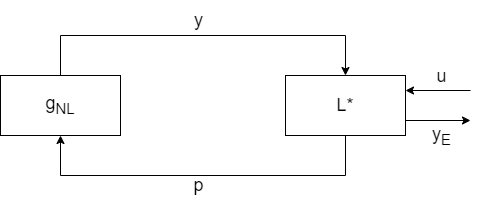
\includegraphics[scale=0.5]{figures/py.png}
    \caption{A rendszerből el lett távolítva a késleltetés nélküli rész; ebben a formában már nincs számítási probléma}
\end{figure}

\section{A K-módszer elemzése}\label{bilinearK}

Egy általános kauzális, idő-invariáns rendszernek az általános állapotváltozós leírása az alábbi alakban felírható~\cite{borin}\cite{borin2}\cite{otherK}:
\begin{subnumcases}{\label{avlna}} 
    \mathbf{\dot{w}}=\mathbf{Aw}+\mathbf{Bu}+\mathbf{Cy}\label{kw}\\
    \mathbf{x}=\mathbf{Dw}+\mathbf{Eu}+\mathbf{Fy}\label{kx}\\
    \mathbf{y}=\mathbf{f} (\mathbf{x})\label{ky}
\end{subnumcases}
ahol $w$ az állapotvektor és $u$ a bemenet.
Laplace-transzformálva, majd bilineáris transzformációt alkalmazva (\ref{kw}) egyenletre~\cite{borin}:
\begin{equation}
    s\mathbf{W(s)}=\mathbf{AW}(s)+\mathbf{BU}(s)+\mathbf{CY}(s)
\end{equation}
\begin{equation}
    h\frac{1-z^{-1}}{1+z^{-1}}\mathbf{W}(s)=\mathbf{AW}(s)+\mathbf{BU}(s)+\mathbf{CY}(s)
\end{equation}
ahol $h=\frac{2}{T}$. Ezt rendezve:
\begin{equation}
    h(1-z^{-1})\mathbf{W}(z)=\mathbf{A}(1+z^{-1})\mathbf{W}(z)+(1+z^{-1})(\mathbf{BU}(z)+\mathbf{CY}(z))
\end{equation}
\begin{equation}
    h\mathbf{W}(z)-\mathbf{AW}(z)=z^{-1}h\mathbf{W}(z)+z^{-1}\mathbf{AW}(z)+\mathbf{BU}(z)+\mathbf{CY}(Z)+z^{-1}(\mathbf{BU}(z)+\mathbf{CY}(z))
\end{equation}
\begin{equation}
    (h\mathbf{I}-\mathbf{A})\mathbf{W}(z)=z^{-1}(h\mathbf{I}+\mathbf{A})\mathbf{W}(z)+\mathbf{BU}(z)+z^{-1}\mathbf{BU}(z)+\mathbf{CY}(z)+z^{-1}\mathbf{CY}(z)
\end{equation}
Inverz z-transzformálva:
\begin{equation}
    (h\mathbf{I}-\mathbf{A})\mathbf{w}[n]=(h\mathbf{I}+\mathbf{A})\mathbf{w}[n-1]+\mathbf{Bu}[n]+\mathbf{Bu}[n-1]+\mathbf{Cy}[n]+\mathbf{Cy}[n-1]
\end{equation}
Ha ($h\mathbf{I}-\mathbf{A}$) invertálható (ami igaz lesz mindig, ha $h$ az $\mathbf{A}$ mátrix sajátértékeitől különbözik~\cite{borin}), akkor balról 
az inverzével beszorozva a két oldalt:
\begin{equation}
    \mathbf{w}[n]={(h\mathbf{I}-\mathbf{A})}^{-1}((h\mathbf{I}+\mathbf{A})\mathbf{w}[n-1]+\mathbf{Bu}[n]+\mathbf{Bu}[n-1]+\mathbf{Cy}[n]+\mathbf{Cy}[n-1])
\end{equation}
A könnyebb felírás érdekében új segédváltozók bevezetése ajánlott.
\begin{eqnarray}
    &\mathbf{G} \triangleq {(h\mathbf{I}-\mathbf{A})}^{-1}\mathbf{C}
   \label{G}\\
    &\mathbf{H} \triangleq {(h\mathbf{I}-\mathbf{A})}^{-1}(h\mathbf{I}+\mathbf{A})
   \label{H}\\
    &\mathbf{J} \triangleq {(h\mathbf{I}-\mathbf{A})}^{-1}\mathbf{B}
   \label{J}
\end{eqnarray}
Ezeket behelyettesítve:
\begin{equation}
    \mathbf{w}[n]=\mathbf{Hw}[n-1]+\mathbf{J}(\mathbf{u}[n]+\mathbf{u}[n-1])+\mathbf{Gy}[n-1]+\mathbf{Gy}[n]
\end{equation}
Egy újabb segédváltozó bevezetése:
\begin{eqnarray}
    \mathbf{\hat{p}} \triangleq \mathbf{Hw}[n-1]+\mathbf{J}(\mathbf{u}[n]+\mathbf{u}[n-1])+\mathbf{Gy}[n-1]
   \label{pk}
\end{eqnarray}
Ezt behelyettesítve:
\begin{equation}
    \mathbf{w}[n]=\mathbf{\hat{p}}[n]+\mathbf{Gy}[n]
   \label{wn}
\end{equation}
Az átalakítások segítségével a (\ref{kx}) egyenlet felírható:

\begin{equation}
    \mathbf{x}[n]=\mathbf{D\hat{p}}[n]+\mathbf{DGy}[n]+\mathbf{Eu}[n]+\mathbf{Fy}[n] = \mathbf{p}[n]+\mathbf{Ky}[n]
\end{equation}
ahol
\begin{equation}
    \mathbf{K} \triangleq \mathbf{DG}+\mathbf{F}
   \label{K}
\end{equation}
\begin{equation}
    \mathbf{p}[n] \triangleq \mathbf{D\hat{p}}[n]+\mathbf{Eu}[n]
\end{equation}

Összességében~\cite{borin}:
\begin{equation}
    \begin{cases}
        \mathbf{p}[n]=\mathbf{Hw}[n-1]+\mathbf{J}(\mathbf{u}[n]+\mathbf{u}[n-1])+\mathbf{Gy}[n-1]+\mathbf{Eu}[n] \\
        \mathbf{y}[n]=\mathbf{f}_{NL}(\mathbf{p}[n]+\mathbf{Ky}[n]) \\
        \mathbf{w}[n]=\mathbf{Hw}[n-1]+\mathbf{J}(\mathbf{u}[n]+\mathbf{u}[n-1])+\mathbf{Gy}[n-1]+\mathbf{Gy}[n]
    \end{cases}
   \label{keq}
\end{equation}
A (\ref{keq}) egyenletrendszerben az egyetlen problémát okozó rész a második egyenlet. 
Ezen kívül az egyenletrendszeren sorba iterálva minden elem kiszámolható, hiszen a $\mathbf{p}[n]$ 
csak a definiált és a múltbéli változóértékektől függ, a $\mathbf{w}[n]$ egyenletébe szintén csak be 
kell helyettesíteni az $\mathbf{y}[n]$ kiszámolása után.

Érdemes megjegyezni, hogy ezt a módszert másféle folytonos időből diszkrét időbe transzformációval 
is le lehet vezetni (például hátralépő Euler módszerrel)~\cite{borin}.

\section{A nemlineáris rész}
A korábbi fejezetben látható, hogy a számítási problémát korlátozódik (\ref{keq}) második 
egyenletére:
\begin{equation}
    \mathbf{y}[n]=\mathbf{f}_{NL}(\mathbf{p}[n]+\mathbf{Ky}[n])
   \label{nonlineq}
\end{equation}
A cél az egyenletek rendezésével az volt, hogy olyan formára legyen hozva a megoldandó számítási 
problémát okozó egyenlet, hogy arra alkalmazható legyen a Dini-tételt.
\subsection{Dini-tétel}\label{dini}
A Dini-tételnek csak a SISO rendszerekre vonatkoztatott alakját tárgyalja ez a dokumentum (MISO és 
MIMO rendszerekre is meg lehet fogalmazni~\cite{borin}). Adott egy implicit függvény: 
\begin{equation}
    f(x,y)=0
\end{equation}
Ha ennek a függvénynek létezik olyan pontja, amelyre igaz egy $P_0(x_0, y_0)$ pontban, hogy
\begin{equation}
    \frac{\partial{f}}{\partial{y}}\biggr |_{(x_0, y_0)} \neq 0
   \label{partial}
\end{equation}
akkor létezik olyan $g(x)$ függvény, amelyre
\begin{equation}
    f(x, g(x))=0
\end{equation}
igaz a $P_0$ pont körül. Könnyen belátható, hogy (\ref{partial}) nem csak $P_0$-ra, hanem az egész 
$f(x,y)$ függvényre igaz, akkor $f(x,y)$ nem csak lokálisan, hanem globálisan is kifejezhető 
$f_{NL}(x,g(x))$ függvénnyel~\cite{borin}.

Ebben az esetben az $f(x,y)$ függvény a (\ref{nonlineq}) nullára rendezett alakja:
\begin{equation}
    f_{NL}(p+ky)-y=0
\end{equation}
Ha az y szerinti parciális deriváltjára adott a feltétel, azaz
\begin{equation}
    \frac{\partial{f}}{\partial{y}}=f'_{NL}(p+ky)k-1 \neq 0
\end{equation}
\begin{equation}
    f'_{NL}(p+ky) \neq \frac{1}{k}
\end{equation}
akkor létezik $g(p)$, amelyre
\begin{equation}
    g(p)=y
\end{equation}
Mivel ismerjük az $f(x)=y$ függvényt, ezért geometriai megfontolások 
miatt~\cite{borin} a $g(p)$ függvényt az $f(x)$ függvény lineáris transzformációjával 
kapható meg, mégpedig a
\begin{equation}
    \begin{cases}
        y=y_s \\
        p=x-ky
    \end{cases}
\end{equation}
lineáris transzformáció segítségével, ami az $(x,y)$ síkból a $(p,y_s)$ síkba transzformál.

\section{A K-módszer alkalmazása}
A korábban már levezetett (\ref{keq}) szerint:
\begin{equation}
    \begin{cases}
        \mathbf{p}[n]=\mathbf{Hw}[n-1]+\mathbf{J}(\mathbf{u}[n]+\mathbf{u}[n-1])+\mathbf{G}\mathbf{y}[n-1]+\mathbf{Eu}[n] \\
        \mathbf{y}[n]=\mathbf{f}_{NL}(\mathbf{p}[n]+\mathbf{Ky}[n]) \\
        \mathbf{w}[n]=\mathbf{Hw}[n-1]+\mathbf{J}(\mathbf{u}[n]+\mathbf{u}[n-1])+\mathbf{Gy}[n-1]+\mathbf{Gy}[n]
    \end{cases}
\end{equation}
Ha ez az egyenletrendszert a korábban bevezetett változók szerint kerül felírásra, akkor ezeken 
végigiterálva a nemlineáris rendszer egyenleteinek megoldása lesz az eredmény~\cite{borin}.
\begin{equation}
    \begin{cases}
        \mathbf{\hat{p}}[n]=\mathbf{Hw}[n-1]+\mathbf{J}(\mathbf{u}[n]+\mathbf{u}[n-1])+\mathbf{Gy}[n-1] \\
        \mathbf{p}[n]=\mathbf{D\hat{p}}[n]+\mathbf{Eu}[n] \\
        \mathbf{y}[n]=\mathbf{g}(\mathbf{p}[n]) \\
        \mathbf{w}[n]=\mathbf{Gy}[n]+\mathbf{\hat{p}}[n]
    \end{cases}
   \label{iter}
\end{equation}
A (\ref{iter}) egyenletrendszer harmadik egyenlete megoldható például egy előre legenerált 
táblázat szerint, amiben az $(p,y)$ értékpárokat tároljuk le, és ezek közül lesznek az értékpárok kikeresve. 
Ez a rész fogja a K-módszer hatékonyságát adni, hiszen így nem valós időben kell egy 
implicit egyenletrendszert megoldani, hanem egy előre legenerált táblázatból elég kikeresni 
az eredményt.\\
Összefoglalva az algoritmus lépéseit~\cite{otherK}:
\begin{enumerate}
    \item $\mathbf{\hat{p}}[n]$ kiszámolása (\ref{pk}) szerint
    \item $\mathbf{p[n]}$ kiszámítása $\mathbf{\hat{p}}[n]$ és $\mathbf{u}[n]$ felhasználásával
    \item $\mathbf{y[n]}$ kiszámítása a letárolt táblázatban való kereséssel
    \item Az állapotáltozók ($\mathbf{w}$) frissítése (\ref{wn}) szerint
    \item A kimenet kiszámolása $\mathbf{w}[n]$, $\mathbf{u}[n]$, $\mathbf{y}[n]$ segítségével
\end{enumerate}

\section{Példa}
A módszer bemutatása céljából a Tube-Screamer áramkörének a ``clipping stage``részét valósítottam meg K-módszer segítségével. 

\begin{figure}[H]
    \centering
    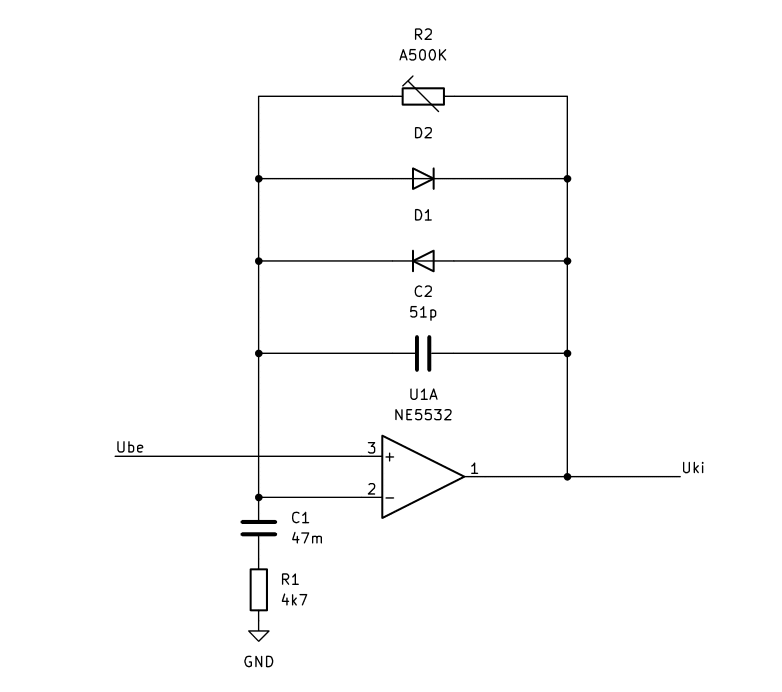
\includegraphics[scale=0.9]{figures/TSCS.png}
    \caption{A Tube-Screamer áramkör ``clipping stage``részének áramköre}
\end{figure}

\subsection{Megvalósítás}
Először meg kell határozni a rendszer állapotváltozós leírását. Az állapotváltozóknak a kondenzátorok 
feszültségét veszem fel. A diódákat összevonom, és egy nemlineáris elemként kezelem. A nemlineáris 
függvény pedig a két diódakarakterisztika összege lesz. A Kirchoff-törvényekből felírt egyenleteket 
átrendezve:
\begin{equation}
    \begin{cases}
        u_{C1}'=-\frac{1}{R_1C_1}u_{C1}+\frac{1}{R_1C_1}u_{be} \\
        u_{C2}'=-\frac{1}{C_2R_1}u_{C1}-\frac{1}{C_2R_2}u_{C2}+\frac{1}{C2R1}u_{be}-\frac{1}{C_2}f(u_{C2}) \\
        f(u)=I_{S0}(e^{\frac{u}{u_T}}-e^{\frac{-u}{u_T}}) \\
        u_{ki}=u_{C2}+u_{be}         
    \end{cases}
   \label{diodak}
\end{equation}
A K-módszerhez szükséges mátrix alakban felírva:
\begin{equation}
    \begin{cases}
        \mathbf{\dot{w}}=
    \begin{pmatrix}
        -\frac{1}{R_1C_1} & 0 \\
        -\frac{1}{C_2R_1} & -\frac{1}{C_2R_2}
    \end{pmatrix}
    \mathbf{w}+
    \begin{pmatrix}
        \frac{1}{R_1C_1} \\
        \frac{1}{C2R1}
    \end{pmatrix}
    u+
    \begin{pmatrix}
        0 \\
        -\frac{1}{C_2}
    \end{pmatrix}
    y \\
    x=
    \begin{pmatrix}
        0 & 1
    \end{pmatrix}
    w \\
    y=f(x)
    \end{cases}
\end{equation}
Az ebből meghatározott mátrixok:
\begin{equation}
    \begin{array}{c}
        \mathbf{A}=
    \begin{pmatrix}
        -\frac{1}{R_1C_1} & 0 \\
        -\frac{1}{C_2R_1} & -\frac{1}{C_2R_2}
    \end{pmatrix}
\quad  
\mathbf{B}=
    \begin{pmatrix}
        -\frac{1}{R_1C_1} & 0 \\
        -\frac{1}{C_2R_1} & -\frac{1}{C_2R_2}
    \end{pmatrix}
\quad 
\mathbf{C}=
    \begin{pmatrix}
        0 \\
        -\frac{1}{C_2}
    \end{pmatrix} \\ 
    \\ 
    \mathbf{D}=
    \begin{pmatrix}
        0 & 1
    \end{pmatrix}
\quad  E=0\quad F=0
    \end{array}
\end{equation}
A segédváltozókat kiszámolom a (\ref{G}), (\ref{H}), (\ref{J}), (\ref{K}) egyenletekkel. 

Legenerálom az $f(u)$ függvény táblázatát, majd végrehajtom rajta az $y_s=y$, 
$p=x-Ky$  lineáris transzformációt. Lehetőség szerint érdemes csak a valóságban is előforduló 
két szélsőérték határán belüli értékeket legenerálni, illetve ha az $y$ tengelyre szimmetrikus a függvényünk, 
akkor csak az egyik oldalt letárolni (ennél a példánál ez pont lehetséges).
Ezután már csak futtatni kell a (\ref{iter}) pontban leírt algoritmust.

\subsection{Eredmény}
Az áramkört az LTSpice programban is elkészítettem összehasonlítás céljából, és teszteltem a K-módszert 
a fent említett függvénnyel, illetve LTSpice-ból kiexportált karakterisztikával.

\begin{figure}[!h]
    \centering
    \begin{subfigure}{0.47\textwidth}
        \centering
        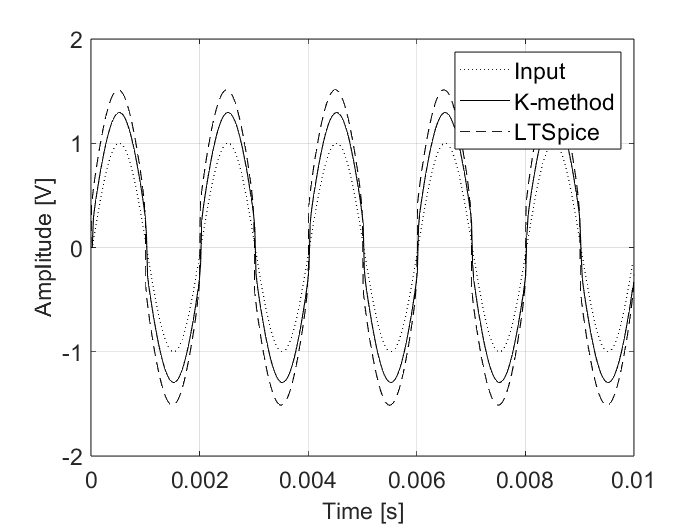
\includegraphics[scale=0.38]{figures/ownmodel.png}
        \caption{A (\ref{diodak}) egyenletben leírt karakterisztikával}\label{a}
    \end{subfigure}
    \hfill
    \begin{subfigure}{0.47\textwidth}
        \centering
        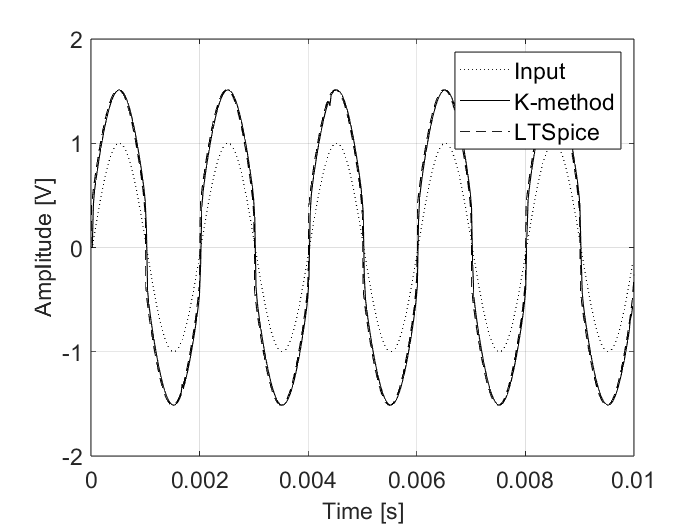
\includegraphics[scale=0.38]{figures/spicemodel.png}
        \caption{LTSpice-ból exportált karakterisztikával}\label{b}
    \end{subfigure}
    \caption{A megvalósított modell válaszjele egy $500 Hz$ frekvenciájú, $1 V$ amplitúdójú szinusz 
    jelre}
\end{figure}
A (\ref{diodak}) egyenletrendszerben említett karakterisztikával az eredmény eltér az LTSpice program által 
meghatározott kimenettől, ami a (\ref{a}) ábrán látható. A jelalakok hasonlóak, viszont amplitúdóban különböznek. Ez 
azért van, mert az LTSpice nem ugyan ezzel a karakterisztikával számol. Erre abból lehet következtetni, hogy 
ha az LTSpice-ból exportáljuk a karakterisztikánkat, akkor a kimenetek megegyezőek lesznek, ahogy látható a (\ref{b}) ábrán is.
\chapter{A K-módszer összehasonlítása más állapotteres módszerekkel}

Áramkör szimulációt több megközelítéssel is meg lehet megvalósítani. Ezek a megközelítések három nagy csoportba sorolhatóak: állapotteres módszerek, digitális hullámszűrő módszer és a fekete doboz módszerek~\cite{book}. Ebben a fejezetben az állapotteres módszerek közül a K-módszert és a legeltejedtebb, valós idejű szimulációnál használt állapotteres módszereket fogom összehasonlítani.

\section{Az állapotteres módszerek}

Az állapotteres módszerek kiindulási alapja, hogy az áramkörnek szükséges felírni az állapotváltozós leírását:
\begin{equation}
    \mathbf{\dot{w}}=\mathbf{Aw}(t)+\mathbf{Bu}(t)+\mathbf{Cf}(\mathbf{Dw}(t)+\mathbf{Eu}(t)+\mathbf{Ff}(\ldots))
    \label{avlnaTDK}
\end{equation}
Az egyenletrendszerben a $\mathbf{w}$ az állapotvektor, $\mathbf{u}$ a gerjesztés, $\mathbf{f}$ pedig egy nemlineáris függvény.

Ezután diszlretizálásra van szükség. Ez két különböző módon is megtehető: vagy a fentebb említett deriváltat egyből helyettesítjük az azt közelítő kifejezéssel, vagy ha az nem kifejezhető, akkor Laplace-transzformáció után az $s$ tartományból behelyettesítéssel áttérünk a $z$ tartományba, majd rendezés után inverz-z transzformálva megkapjuk a diszkretizált állapotegyenletet.

Laplace-transzformáció esetén az egyenletrendszer alakja:
\begin{equation}
    s\mathbf{W}(s)=\mathbf{AW}(s)+\mathbf{BU}(s)+\mathbf{Cf}(\mathbf{DW}(s)+\mathbf{EU}(s)+\mathbf{Ff}(\ldots))
\end{equation}

Leggyakrabban az állapotteres módszerek a diszkretizálásban fognak különbözni, hiszen kulcsfontosságú, hogy hogyan fogják a deriváltat közelíteni. Ez fogja meghatározni a diszkrét rendszer stabilitását, hatása lesz a számítási igényre (a kifejezés bonyolultsága), és a hiba nagyságát, amivel eltér az analóg rendszertől (referencia a fejezetre ahol be vannak mutatva).
\begin{equation}
    s \approxeq l(z)
\end{equation}
Ezt behelyettesítve:
\begin{equation}
    l(z)\mathbf{W}(z)=\mathbf{AW}(z)+\mathbf{BU}(z)+\mathbf{Cf}(\mathbf{DW}(z)+\mathbf{EU}(z)+\mathbf{Ff}(\ldots))
\end{equation}
Inverz z-transzformáció és rendezés után az egyenlet alakja:
\begin{equation}
    \mathbf{w}[n]=\sum_{i = 1}^{M}  \mathbf{H}_i \mathbf{w}[n-i]+\sum_{j=0}^{N}\mathbf{J}_j \mathbf{u}[n-j]+\sum_{k=0}^{P}\mathbf{G}_k \mathbf{f(\mathbf{Dw}[n-k] +\mathbf{Eu}[n-k]+\mathbf{Ff}(\ldots))}
\end{equation}

\subsection{Euler-módszerek}

Az előrelépő- és hátralépő Euler-módszert gyakran alkalmazzák a gyakorlatban (sok ref), de valós idejű szimuláció esetén csak a hátralépő Euler-módszer alkalmazható, hiszen nagyon gyakran a stabilitási feltételnek (\ref{fwEulerSection}) teljesüléséhez nagy mintavételi frekvenciára van szükség.

A hátralépő Euler-módszerben a diszkretizálás után az egyenlet mindig implicit lesz, így azt valamilyen numerikus zérushelykereső módszerrel kell megoldani (\ref{bwEulerSection}). 

Ha az $\mathbf{F}$ változó a (\ref{avlnaTDK}) egyenletben nem $0$, akkor nem elég egy numerikus zérushelykereső algoritmus az egyenlet megoldásához.

Ekkor az egyenlet alakja:
\begin{equation}
    \mathbf{w}[n]=\mathbf{Hw}[n-1]+\mathbf{Ju}[n]+\mathbf{Gf}(\mathbf{Dw}[n]+\mathbf{Eu}[n]+\mathbf{Ff}(\ldots))
\end{equation}
Látható, hogy az egyenlet implicit, hiszen az egyenlet bal oldalán és a függvény argumentumaként is szerepel $\mathbf{w}[n]$. Bonyolultabb áramkörök esetén előfordul, hogy a nemlinearitás visszahat magára (hasonló egy visszacsatoláshoz), és ekkor egy végtelen függvény egymásbaágyazódás figyelhető meg. Ezt a két problémát egyszerre nem tudják kezelni a numerikus zérushelykereső módszerek, így más megközelítés szükséges.

Egy lehetőség a megoldásra az egyenlet szétválasztása olyan formában, ahogyan azt a K-módszer teszi (\ref{KSep}). Előbb a nemlineáris rész kimenete lesz meghatározva, majd csak utána lesz az állapotvektor kiszámolva és aktuális értékeire frissítve.

A nemlineáris rész kimenetét elnevezve $y[n]$-nek és a szétválasztott egyenletrendszer felírva:
\begin{equation}
    \begin{cases}
        \mathbf{w}[n]=\mathbf{Hw}[n-1]+\mathbf{Ju}[n]+\mathbf{Gy}[n]\\
        \mathbf{y}[n]=\mathbf{f}(\mathbf{Dw}[n]+\mathbf{Eu}[n]+\mathbf{Fy}[n])
    \end{cases}
\end{equation}
Ez a lépés még nem oldotta meg a problémát, viszont az állapotvektor egyenletét a nemlineáris rendszer kimenetének egyenletébe behelyettesítve $\mathbf{w}[n]$-től független egyenletet kapunk:
\begin{equation}
    \mathbf{y}[n]=\mathbf{f}(\mathbf{D}(\mathbf{Hw}[n-1]+\mathbf{Ju}[n]+\mathbf{Gy}[n])+\mathbf{Eu}[n]+\mathbf{Fy}[n])
\end{equation}
Ezt az egyenletet már képesek a zérushelykereső módszerek megoldani. Megoldás után a nemlineáris rész kimenetét visszahelyettesítve $\mathbf{w}[n]$ egyenletébe megkapjuk az állapotvektor aktuális elemeit.

A K-módszerben is alkalmazott egyenletszétválasztással meg tudtunk oldani egy olyan egyenletet, amiben két probléma van egyszerre jelen: szétválasztás és behelyettesítés után a két problémát külön választottuk, amiket külön-külön meg lehet oldani. Bonyolultabb áramkörökben ezt a plusz lépést gyakran végre kell hajtani.

\subsection{K-módszer}
A K-módszer az egyenletek szétválasztásával kezd, függetlenül az $\mathbf{F}$ változótól. Szétválasztás után ugyanúgy a nemlineáris rész kimenetét számolja ki először, de ehhez nem numerikus zérushelykereső módszert használ, hanem alkalmazza a Dini-tételt~\cite{borin}, ami kimondja, hogy egy implicit függvényhez található egy olyan explicit pár, ami ha néhány feltétel teljesül, akkor meg fognak egyezni~(\ref{dini}).

Ezt az explicit függvényt ki lehet offline számolni, letárolni egy tömbben, és így meg lehet oldani az egyenletet egy tömbben való kereséssel a numerikus zérushelykereső módszer helyett.

Érdemes megjegyezni, hogy mivel a Dini-tétel alkalmazásának az a feltétele, mint a Newton-módszernek, így csak akkor lehet alkalmazni, ha a Newton-módszerrel is meg lehetne oldani az egyenletet~\cite{otherK}.

\section{Számítási igény}

Valós idejű szimuláció esetén kritikus fontossággal bír a választott módszer számítási igénye, hiszen megadott időkereten belül kell a kimenetet kiszámolni.

\subsection{Hátralépő Euler-módszer}

$\mathbf{F}=0$ esetén a módszer a Newton-módszer számítási igényével és az előtte elvégzett műveletekkel egyezik meg. A Newto-módszer számítási igénye $O((\log{n})F(n))$, ahol $F(n)$ a $\mathbf{f(x)/\dot{f}(x)}$ kiszámolásának számítási igénye $n$ számjegyű pontosság esetén~\cite{wikiNewton}. Az előtte elvégzett műveletek 3 szorzásból és egy összeadásból állnak ($\mathbf{Hw}[n-1]+\mathbf{Ju}[n]$, és $\mathbf{Eu}[n]$), amiknek számításigényük $O(3n^2)$ és $O(n)$. 

$\mathbf{F} \neq 0$ esetén a Newton-módszer számításigénye, az azelőtt ($\mathbf{DHw}[n-1]+\mathbf{(DJ+E)u}[n]$, és $\mathbf{DG+F}$ kiszámítása), és az azután kiszámolt értékek számításigénye. A Newton-módszer számítási igénye a fentebb említett $O((\log{n})F(n))$. A Newton-módszer előtti műveletek 6 szorzásból, 3 összeadásból állnak, amelyeknek $O(6n^2)$ és $O(6n)$ a komplexitásuk. A Newton-módszer után elvégezendő három szorzásé $O(3n^2)$, a két összeadásé pedig $O(2n)$, $n$ számjegy esetén.

\begin{center}
    \begin{tabular}{ |c|c|c|c|c| } 
     \hline
      & \bf{előtt} & \bf{Newton-módszer} & \bf{után} & \bf{összesen} \\ 
     \hline
     $\mathbf{F}=0$ & \makecell{$3O(n^2) + O(n)$ \\ $=O(n^2)$} & $O((\log{n})F(n))$ & - & $O((\log{n})F(n))$ \\ 
     \hline
     $\mathbf{F}\neq0$ &  \makecell{$6O(n^2)+6O(n)$ \\ $=O(n^2)$} & $O((\log{n})F(n))$ & \makecell{$3O(n^2)+2O(n)$ \\ $=O(n^2)$} & $O((\log{n})F(n))$\\ 
     \hline
    \end{tabular}
\end{center}

A táblázatból látszik, hogy a hátralépő Euler-módszer komplexitását mindig a nemlineáris függvény, és annak deriváltja fogja meghatározni (ha már található benne szorzás művelet, akkor komplexitása minimum $O((\log{n})n^2)$).

\subsection{K-módszer}

A K-módszert numerikus zérushelykereső algoritmus ugyan azt a számításigényt eredményezne, hiszen a két algoritmus között a különbség a diszkretizálási módszer lenne, ami csak összeadás és szorzás műveleteket adna a komplexitáshoz.

A nemlineáris egyenlet megoldása előtt 4 szorzás és 4 összeadás található, komplexitásuk $4O(n^2)$ és $4O(n)$.

Offline tömbbe letárolás esetén csak az abban való keresés lesz, ami számításigényt igényel szemben az állandó hányados számítással a Newton-módszerben. A tömböt legenerálni rendezetten érdemes, ekkor a legrosszabb esetben $m$ elem esetén egy bináris keresés $\log_2 m$ iteráció alatt talál meg.

Az összehasonlítások $n$ számjegy esetén $O(n)$ komplexitásúak, és a keresés lefutása után  3 szorzás és 3 összeadás található, amiknek $3O(n^2)$ és $3O(n)$ a komplexitásuk.

\begin{center}
    \begin{tabular}{ |c|c|c|c| } 
     \hline
      \bf{előtt} & \bf{Bináris keresés} & \bf{után} & \bf{} \\ 
     \hline
     \makecell{$4O(n^2) + 4O(n)$ \\ $=O(n^2)$} & $O(n\log{m})$ & \makecell{$3O(n^2) + 3O(n)$ \\ $=O(n^2)$} & $O(n^2)$ \\ 
     \hline
    \end{tabular}
\end{center}

A K-módszernek a komplexitása $O(n^2)$, hiszen a tömb nagyságát növelve logaritmikusan nő a számítás igény, ami még $32$ bites float pontosság esetén is utólérhetetlen az m nagyságával, hogy a $O(n\log{m})$ domináljon. Az $O(n^2)$-es futásidő a~\cite{book} irodalomban is megtalálható levezetés nélkül.

\section{Az összehasonlítás összefoglalása}
A K-módszer előnyei a hátralépő Euler-módszerrel szemben:
\begin{itemize}
    \item A hátralépő Euler-módszer nagyobb számítási igényű, mint a K-módszer ($O(n^2) < O((\log{n})F(n))$)
    \item A K-módszer pontosabb, mivel pontosabban közelíti a deriváltat a hátralépő Euler-módszernél, és lehetőséget ad nagyobb fokú közelítések használatához is
    \item A hátralépő Euler-módszer végrehajtási menete függ az állapotváltozós leírás alakjától, ezzel szemben a K-módszer mindig ugyan azt a sémát használja
    \item A K-módszerben a letárolt tömb méretét lehet optimalizálni: $y$ tengelyre szimmetrikus függvény esetén elég csak a pozitív x értékek eltárolása, a tömb méretének csökentésével megjelenő pontatlanságot interpolációval egyensúlyozhatjuk, illetve lineáris interpoláció esetén a lineáris részeket lehetőségünk van ritkábban letárolni
\end{itemize}
A hátralépő Euler-módszer előnyei a K-módszerrel szemben:
\begin{itemize}
    \item Kevesebb memóriát foglal futás közben (a K-módszer által letárolt tömböt végig a futás során meg kell tartani)
    \item Ha a modellezett részáramkörben található változtatható paraméter (potméter, érzékelők stb.), akkor minden egyes változásnál a K-módszernél ki kell számolni a mátrixokat és a letárolandó tömböt
    \item A tömb legenerálása előtt meg kell győződni arról, hogy milyen reális maximum és minimum értékek lehetségesek a nemlineáris rész kimeneteként
\end{itemize}
A két módszer egyező tulajdonságai:
\begin{itemize}
    \item Mindkét módszer alkalmazási feltételhez kötött (ez a feltétel gyakran teljesül a zenei alkalmazáshoz tervezett áramkörökben)
\end{itemize}




\chapter{A K-módszer lehetséges felhasználási területei}
A zenei alkalmazásokon kívül az élet sok területén használják a hátralépő Euler-módszert a közönséges differenciálegyenletek megoldásához. Ezek a differenciálegyenletek jól leírják a szimulálandó rendszert, és szimulálásuk során előre észrevehetőek hibák, amit lehet csak a prototípus gyártás után vettek volna észre, a rendszer különböző gerjesztésekre való reagálásának elemzését teszi lehetővé, illetve a különböző rendszerparaméterek megválasztását segítheti. 

\section{Épületszerkezet tervezés, tesztelés}
Az építőmérnöki szerkezettervezés során a hátralépő Euler-módszert az épületek, hidak teszteléséhez használják különböző terhelések esetén~\cite{structeng}. Szeizmikus, vagy akár szélterhelést szimulálva a dinamikai viselkedés vizsgálható, tesztelve így annak stabilitását és biztonságosságát.

\section{Reakciókinetika}
A reakciókinetikában a hátralépő Euler-módszert alkalmazzák a reakciósebességek és a reaktánsok, valamint a termékek koncentrációinak modellezésére kémiai folyamatokban~\cite{chemeng}.

\section{Pénzügy}
A pénzügyben a hátralépő Euler-módszert szokták használni opció árazási modellekben, amikben felmerülnek differenciálegyenletek~\cite{finance}.

\\

A felsoroltakon kívül még számos területen alkalmazzák a hátralépő Euler-módszert. Érdemes lenne helyette a K-módszert használni, már csak amiatt, hogy az eredmények pontosabbak legyenek a bilineáris transzformáció alkalmazásának köszönhetően. Emellett pedig ha fontos szempont a valós idejűség, akkor már a kisebb számítási igény miatt is megérné a K-módszert használni.   
\chapter{Gitárerősítő modellezése}
A félév során az Orange Crush 20L gitárerősítőt modelleztem. Az áramkört az LTSpice segítségével teszteltem. A műveleti erősítőket ideálisnak vettem ott, ahol a valóságnak megfelelő jel esetén nem tapasztaltam levágást, ahol pedig tapasztaltam, ott egy egyszerű levágó algoritmussal modelleztem ezt a jelenséget \cite{opampo}. A frekvenciafüggő átviteltől és a slew rate-től eltekintettem, hiszen modellezésük ilyen komplex rendszer esetén nem fog nagy hangzásbeli különbséget eredményezni.
\begin{figure}[H]
    \centering
    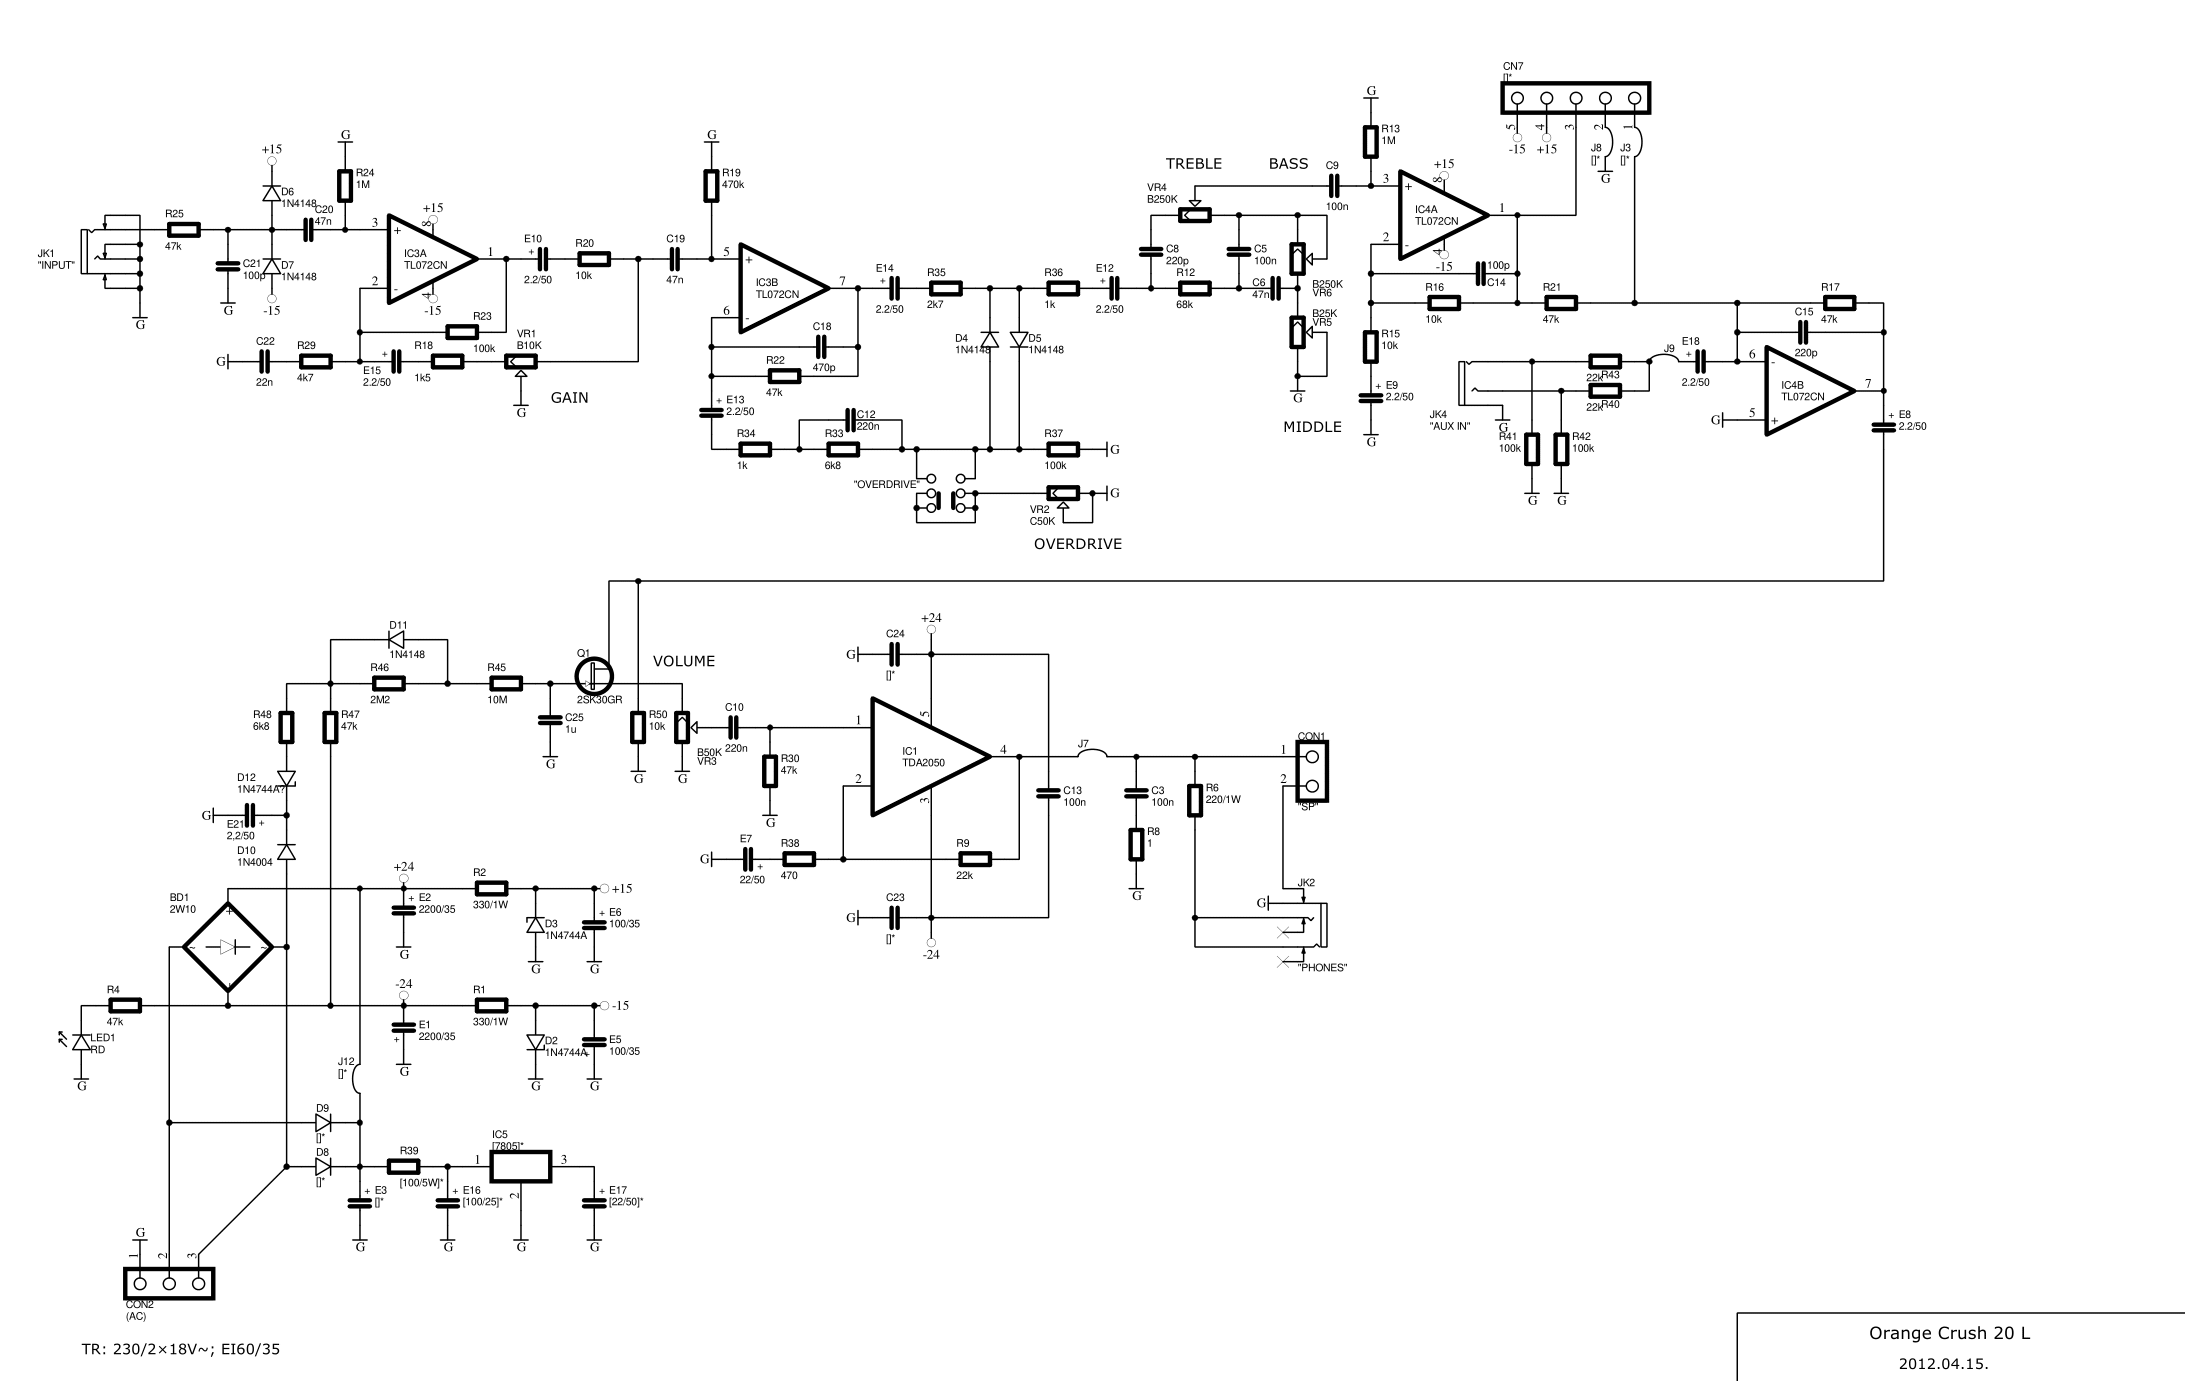
\includegraphics[scale=0.50]{figures/orange_crush_20l_guitar_amp_sch-1.png}
    \caption{Az Orange Crush 20L erősítő áramköre}
\end{figure}

Az áramkört a műveleti erősítők bemeneténél és kimeneténél részekre bontottam, hiszen a műveleti erősítőnek 
nagyimpedanciás bemenete és kisimpedanciás a kimenete, ami miatt az előtte lévő áramköri elemeket nem terheli 
meg, illetve az utána lévő áramkörök nem terhelik meg a műveleti erősítő köré épített részt.
\begin{figure}[H]
    \centering
    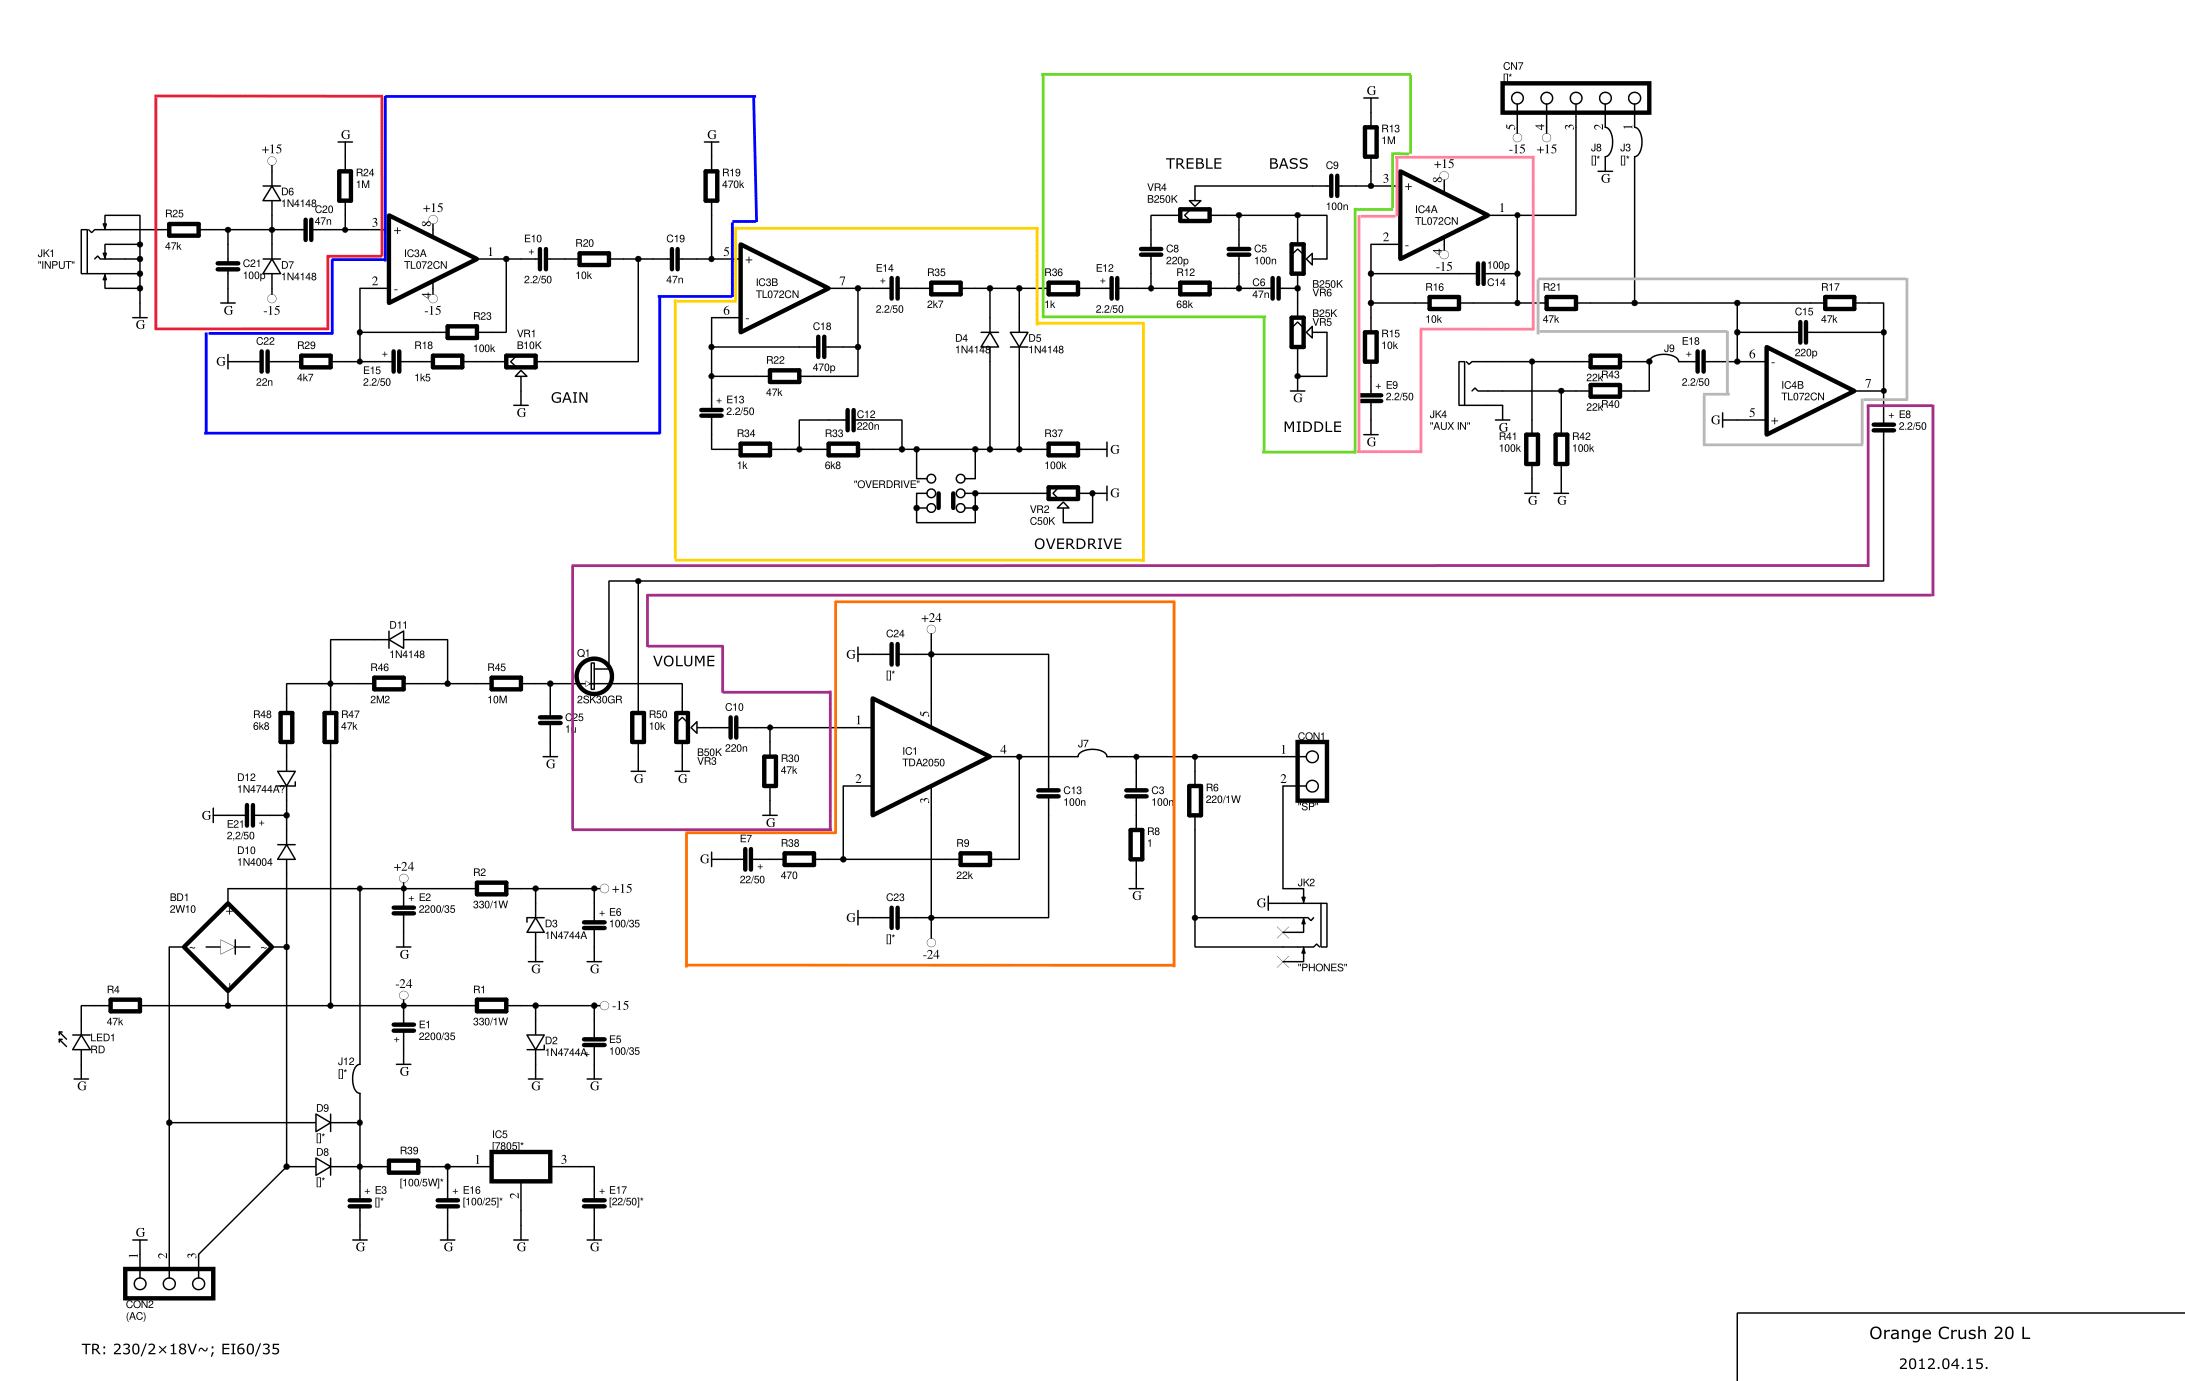
\includegraphics[scale=0.50]{figures/orange_crush_20l_guitar_amp_sch_parts-1.png}
    \caption{Az Orange Crush 20L erősítő áramköre részekre bontva}
\end{figure}
\section{Részáramkörök elemzése}
\subsection{Bemeneti szűrő}

\begin{figure}[H]
    \centering
    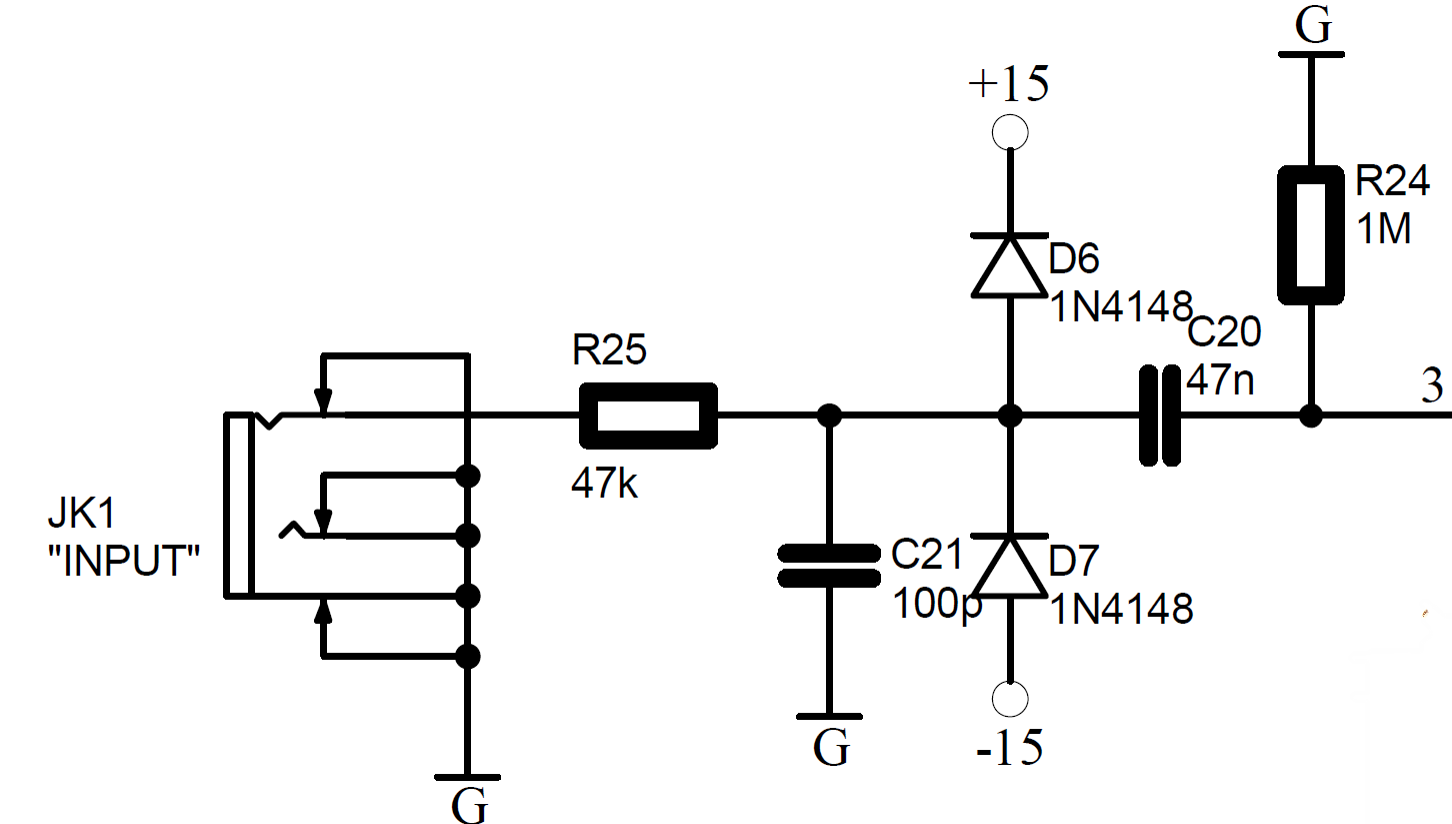
\includegraphics[scale=0.3]{figures/stage1.png}
    \caption{A bemeneti szűrők}
\end{figure}

A bemeneti szűrő egy alul- és egy felüláteresztő RC szűrőből áll. A diódák csak védelem miatt vannak, hogy a 
műveleti erősítő bemenetére ne kerüljön semmiféle módon több feszültség, mint a tápfeszültsége, ezért a 
modellezésben elhanyagolhatjuk.

A hálózatot bilineáris transzformációval modellezve az alábbi eredményeket kaptam az LTSpice szimulációval összehasonlítva:
\begin{figure}[H]
    \centering
    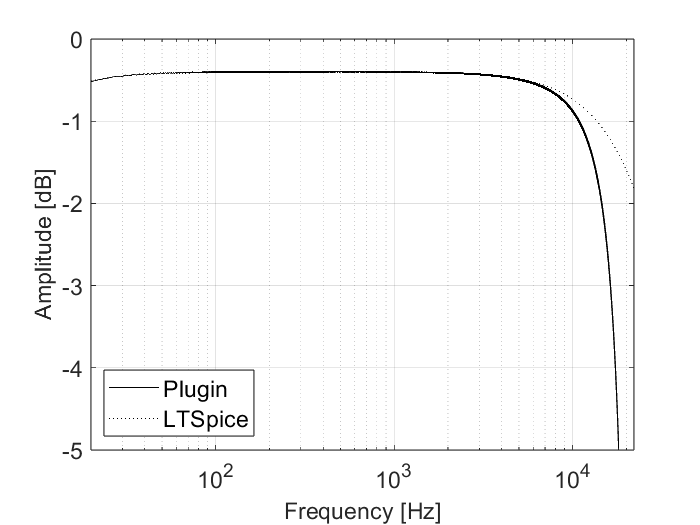
\includegraphics[scale=0.5]{figures/stage1plot.png}
    \caption{Az LTSpice szimuláció eredménye összehasonlítva a megvalósított szűrővel}
\end{figure}

A különbség a bilineáris transzformációnak köszönhető, hiszen egy bilineárisan transzformáció segítségével létrehozott 
diszkrét idejű rendszer a mintavételi frekvenciához 
közeli frekvenciákon jelentősen el tud térni az eredeti folytonos idejű rendszertől. 
Mint látható, hogy a frekvenciamenetek megegyeznek körülbelül $6kHz$-ig, 
és a $6dB$ különbséget pedig jóval $18kHz$ után éri el.

\section{Erősítő rész}
\begin{figure}[H]
    \centering
    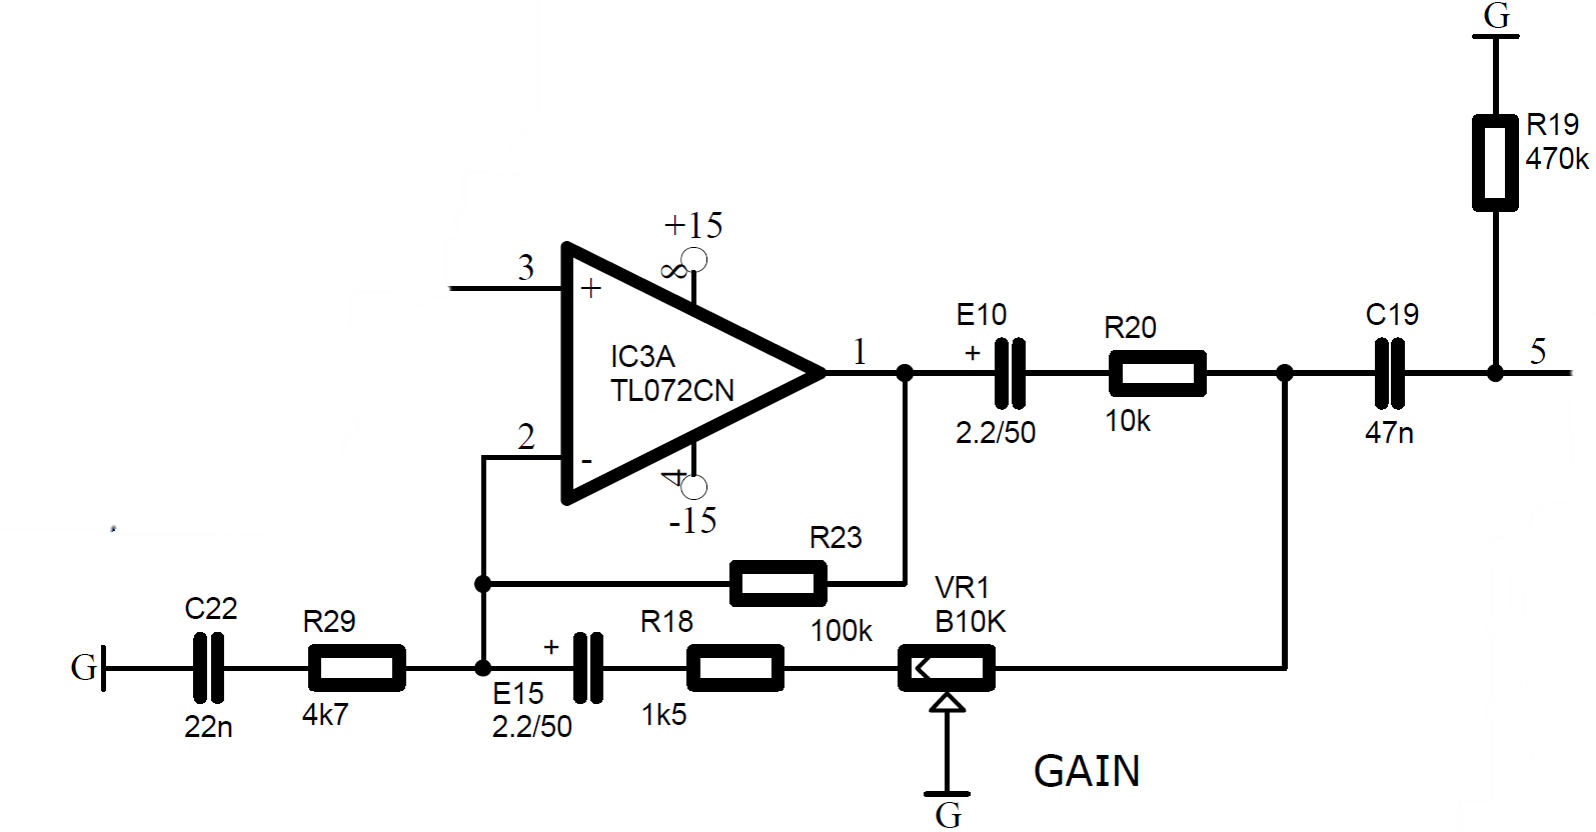
\includegraphics[scale=0.35]{figures/stage2.png}
    \caption{A bemeneti szűrők}
\end{figure}
Az erősítő kimeneténél felbontottam az áramkört (az $1$ pontnál), először a műveleti erősítőt tartalmazó részt 
modelleztem, utána pedig a passzív hálózatot. Mind a két részt bilineáris transzformáció segítségével modelleztem. 

LTSpice szimuláció segítségével észrevettem, hogy a valóságnak megfelelő bemeneti jel esetén is a 
GAIN potméter adott állásaiban le fog vágni a műveleti erősítő a tápfeszültségénél. 

\begin{figure}[H]
    \centering
    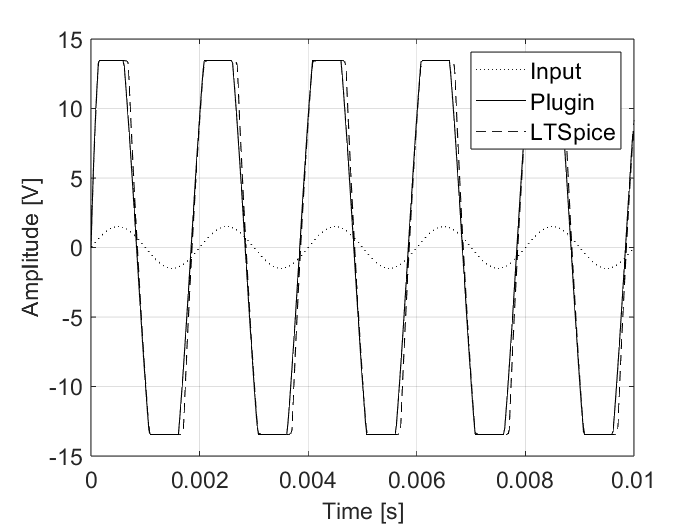
\includegraphics[scale=0.5]{figures/stage2plot.png}
    \caption{A műveleti erősítő válasza egy $500Hz$-es $1.5V$ amplitúdós szinusz jelre}
    \label{again}
\end{figure}

A (\ref{again}) ábrán lehet látni a jelalak minimálisan eltérését az LTSpice szimuláció eredményétől. 
Ez annak köszönhető, hogy az LTSpice-ban lévő műveleti erősítő modell a műveleti erősítő frekvenciafüggését és slew 
rate-jét is figyelembe veszi, illetve valószínűleg sokkal bonyolultabb karakterisztikát használ.

A műveleti erősítő levágását egyszerű levágó algoritmussal valósítottam meg \cite{opampo} \cite{opamp}. Eredetileg az ideális műveleti erősítőt tartalmazó modell fut, és ha annak a kimenete túllépné az LTSpice alapján meghatározott levágási feszültséget, akkor a szarutációs modellel visszaszámolom a bemenetet (ekkor a kimenete a levágási feszültség). A rendszeregyenlet segítségével egyszerűen visszaszámolható a bemenet, azt csak át kell rendezni $u[n]$-re, $y[n]$ adott. Ezután a bufferekben ezek alapján kell frissíteni az értékeket.
\begin{figure}[H]
    \centering
    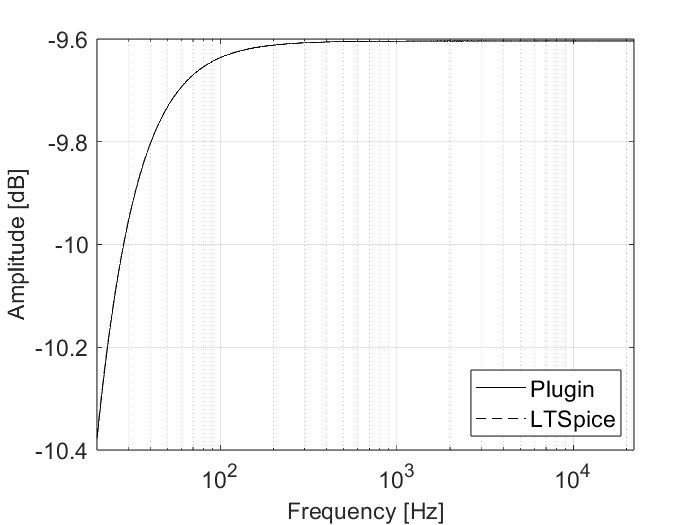
\includegraphics[scale=0.5]{figures/stage2after.png}
    \caption{A műveleti erősítő utáni passzív hálózat tesztelése. A GAIN potméter $5k\Omega$ értékre volt állítva.}
\end{figure}
A passzív hálózat felüláteresztő jellege miatt a bilineáris transzformációval létrehozott modell jól követi a frekvenciamenetet. 

\section{Torzító rész}
\begin{figure}[H]
    \centering
    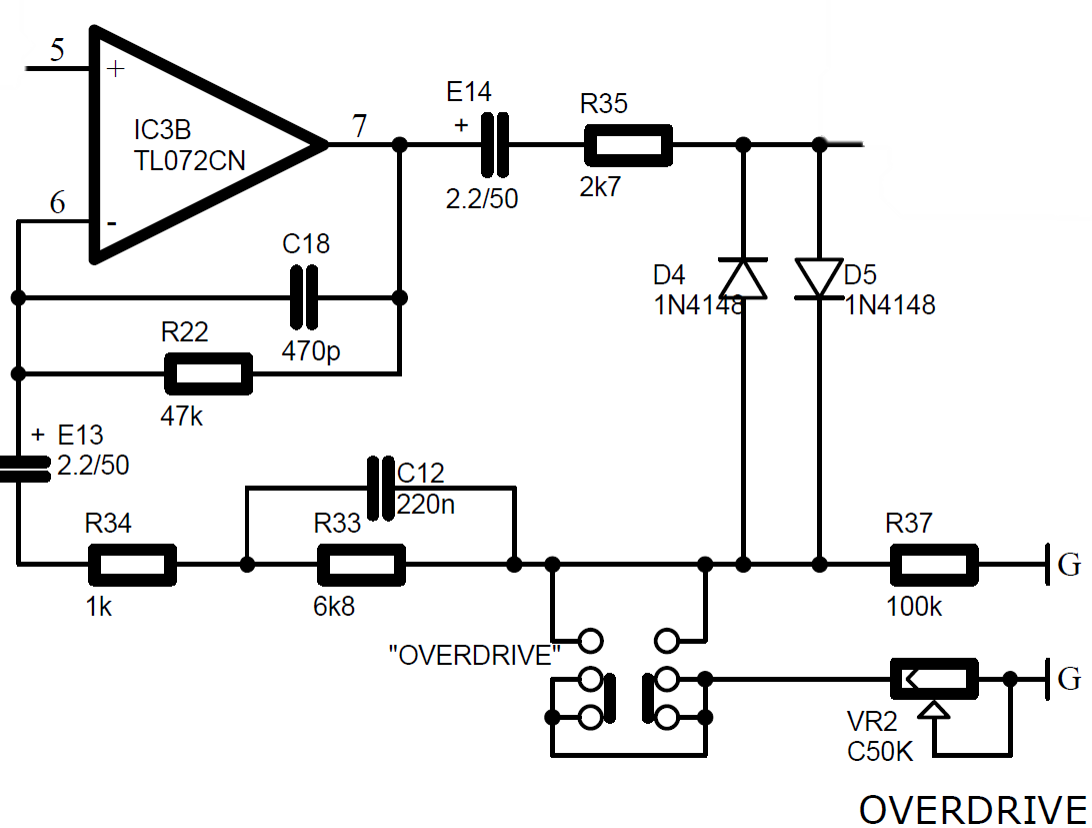
\includegraphics[scale=0.35]{figures/stage3.png}
    \caption{A torzító rész áramköre}
\end{figure}

A torzító rész utáni áramkörrészt leválasztottam, és különböző részként kezeltem. Ezt azért tehettem meg, mert annak a bemeneti impedanciája sokkal nagyobb, mint a torzító rész kimeneti impedanciája, azaz a torzító rész feszültséggenerátorosan hajtja meg az utána következő részeket (ezt LTSpice-ban egy követő erősítő segítségével is teszteltem).
\begin{figure}[H]
    \centering
    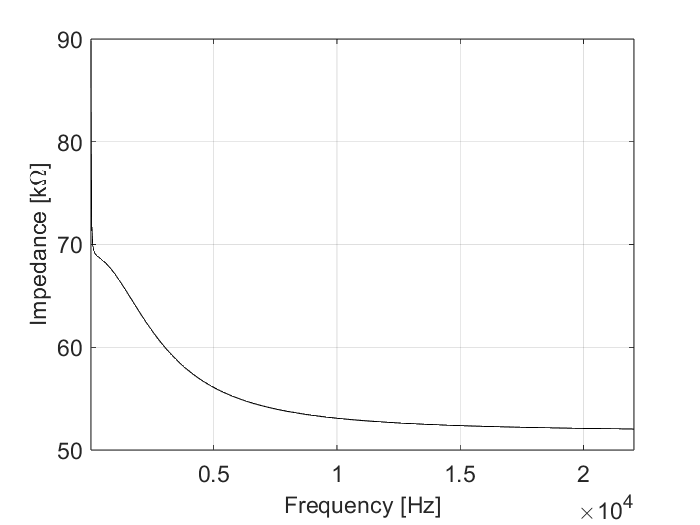
\includegraphics[scale=0.5]{figures/res.png}
    \caption{A torzító részt követő áramkör bemeneti impedanciája}
\end{figure}

A torzító rész modellezéséhez K-módszert használtam, ahol a diódák okozták a nemlinearitást. Tesztelés céljából a táblázatot az általános $i(u)=I_{S0}(1-e^{-\frac{u}{u_T}})$ függvény alapján generáltam le. Ha csak a diódákat vettem bele a nemlineáris függvénybe, akkor nem tudtam kifejezni a kimenetet (hasonló probléma jelenik meg egy feszültségforrásra sorosan kötött dióda és ellenállásnál). A problémát azzal oldottam meg, hogy az $R_{35}$ soros ellenállást is beleszámoltam a nemlineáris függvénybe, és így hoztam létre a táblázatot. Az áramra egy implicit egyenlet jött ki, a feszültségre egy explicit, így a feszültség alapján generáltam le a táblázatot.
\pagebreak
\begin{equation}
    f(u)=i=I_{S0}sinh(\frac{u-R_{35}i}{u_T})
\end{equation}
\begin{equation}
    f^{-1}(i)=u=u_Tsinh(\frac{i}{2I_{S0}})+R_{35}i
\end{equation}
Ezután kiexprotáltam a karakterisztikát ismét LTSpice-ból, és végül ezt használtam majd a végleges eredményhez.

Az LTSpice szimuláció során észrevettem, hogy a műveleti erősítő kimenetén olyan feszültségszintek fordulhatnak elő valósághű bemenetek esetén, amelyeknél meghatározó lesz a műveleti erősítő tápfeszültségének szintje, és le fogja vágni, ha afelé menne. Ennek a modellezése már nem fért bele az Önálló laboratórium tárgyba, viszont egy jó ötlet továbbfejlesztési lehetőségnek. Erre a megoldás egy egyszerű levágó algoritmus lenne \cite{opampo} \cite{opamp}. Az ideális modellel kiszámolnám a műveleti erősítőnknek a kimenetén lévő feszültséget, és ha ez meghaladja a tápfeszültséget, akkor a kimenetére megszabom, abból a bemenetet visszaszámolom, és ez alapján futtatni a K-módszer algoritmusát.\\
Az állapotváltozós leírás alapján kiszámolt mátrixok:
\begin{equation}
    \begin{array}{c}
        \mathbf{A}=
        \begin{pmatrix}
            -\frac{1}{C_{12}(R_{37}+R_{34})}-\frac{1}{C_{12}R_{33}} & 0 & -\frac{1}{C_{12}(R_{37}+R_{34})} & 0 \\
            \frac{1}{C_{18}(R_{37}+R_{34})} & -\frac{1}{R_{22}C_{18}} & \frac{1}{C_{18}(R_{37}+R_{34})} & 0 \\
            -\frac{1}{E_{13}(R_{37}+R_{34})} & 0 & -\frac{1}{E_{13}(R_{37}+R_{34})} & 0 \\
            0 & 0 & 0 & 0
        \end{pmatrix} \\ \\
        \mathbf{B}=
        \begin{pmatrix}
            -\frac{1}{C_{12}(R_{37}+R_{34})} \\
            \frac{1}{C_{18}(R_{37}+R_{34})} \\
            -\frac{1}{E_{13}(R_{37}+R_{34})} \\
            0
        \end{pmatrix} \qquad
        \mathbf{C}=
        \begin{pmatrix}
            \frac{R_{37}}{C_{12}(R_{37}+R_{34})} \\
            1 \\
            -\frac{R_{37}}{R_{37}+R_{34}} \\
            1
        \end{pmatrix} \\ \\
        \mathbf{D}=
        \begin{pmatrix}
            -\frac{R_{37}}{R_{37}+R_{34}} & 1 & -\frac{R_{37}}{R_{37}+R_{34}} & 1 
        \end{pmatrix} \qquad
        E=\frac{R_{34}}{R_{37}+R_{34}} \qquad
        F=-\frac{R_{34}R_{37}}{R_{37}+R_{34}}
    \end{array}
\end{equation}
A (\ref{G}), (\ref{H}), (\ref{J}), (\ref{K}) egyenletekkel kiszámoltam a segédváltozókat, és a (\ref{iter}) lépései szerint programoztam be az algoritmust.Az általam számolt karakterisztikával kapott eredmény a (\ref{nospicenoclip}) és a (\ref{nospiceclip}) ábrán, az LTSpice-ból kiexportált karakterisztikával kapott eredmények pedig a (\ref{spicenoclip}) és (\ref{spiceclip}) ábrán látható.
\begin{figure}[H]
    \centering
    \begin{subfigure}{0.47\textwidth}
        \centering
        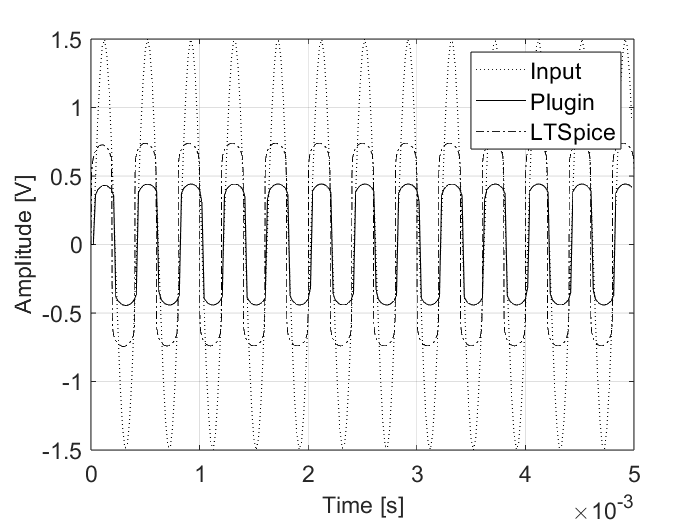
\includegraphics[scale=0.38]{figures/nospicenoclip.png}
        \caption{}
        \label{nospicenoclip}
    \end{subfigure}
    \hfill
    \begin{subfigure}{0.47\textwidth}
        \centering
        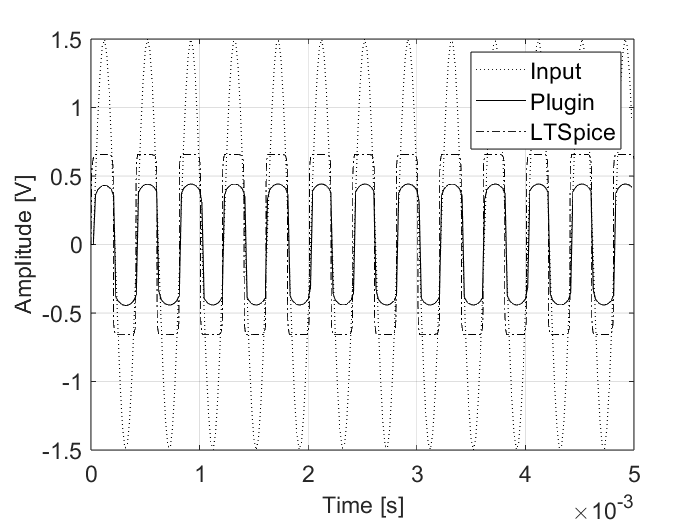
\includegraphics[scale=0.38]{figures/nospiceclip.png}
        \caption{}
        \label{nospiceclip}
    \end{subfigure}
    \begin{subfigure}{0.47\textwidth}
        \centering
        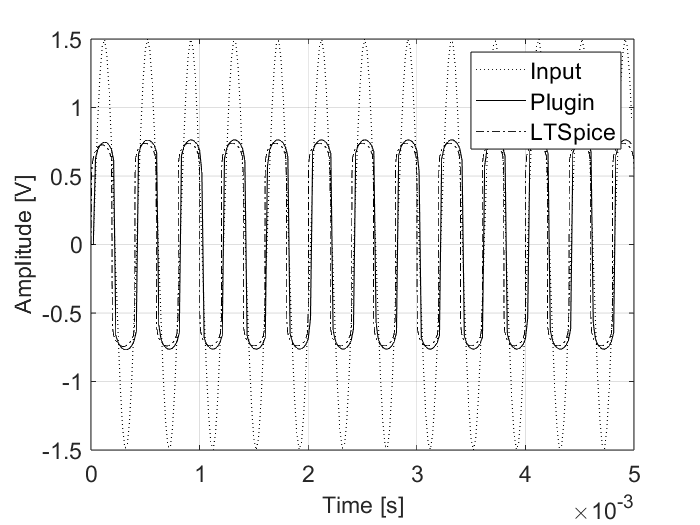
\includegraphics[scale=0.38]{figures/spicenoclip.png}
        \caption{}
        \label{spicenoclip}
    \end{subfigure}
    \hfill
    \begin{subfigure}{0.47\textwidth}
        \centering
        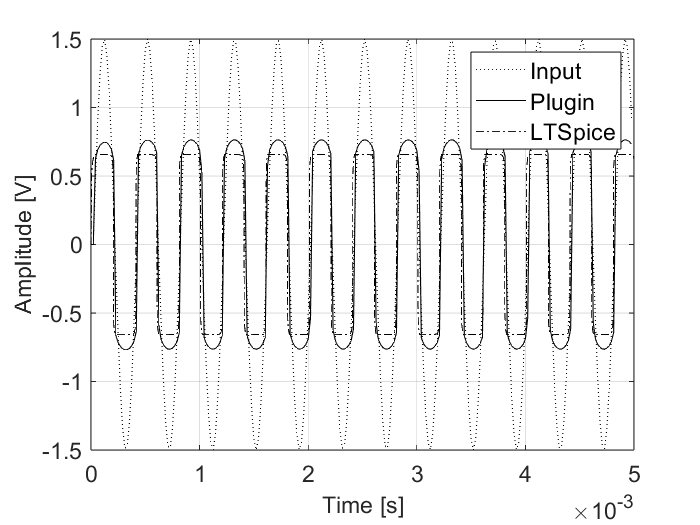
\includegraphics[scale=0.38]{figures/spiceclip.png}
        \caption{}
        \label{spiceclip}
    \end{subfigure}
    \caption{A plugin és az LTSpice által adott válasz, (\ref{nospicenoclip}) és (\ref{spicenoclip}) ábrán amikor az LTSpice-ban ideális műveleti erősítőt használok, és (\ref{nospiceclip}) és (\ref{spiceclip}) ábrán amikor a nem ideális műveleti erősítő modellt használok}
\end{figure}
A megvalósítás során nehézséget okozott az OVERDRIVE paraméter, hiszen minden egyes változásánál változni fognak a segédváltozóink, azaz minden egyes paraméterváltozásnál újra ki kell számolnunk a (\ref{G}), (\ref{H}), (\ref{J}), (\ref{K}) egyenleteket, majd el kell végezni az $f(u)$ függényünkre a lineáris interpolációt (hiszen függ $K$ értékétől). Természetesen amikor a (\ref{iter}) egyenletrendszer lefut, mindig ki lehetne ezt a transzformációt számolni, de egyáltalán nem célszerű. Ezt a problémát a JUCE környezet $juce::AudioProcessorValueTreeState::Listener$ osztályából való örökléssel oldottam meg. Ennek az osztálynak van egy \textit{void parameterChanged(const juce::String\& parameterID, float newValue)} nevű függvénye, ami mindig csak akkor hívódik meg, amikor a hozzá tartozó paraméter értéke változik.
\section{Tone stack}
\begin{figure}[H]
    \centering
    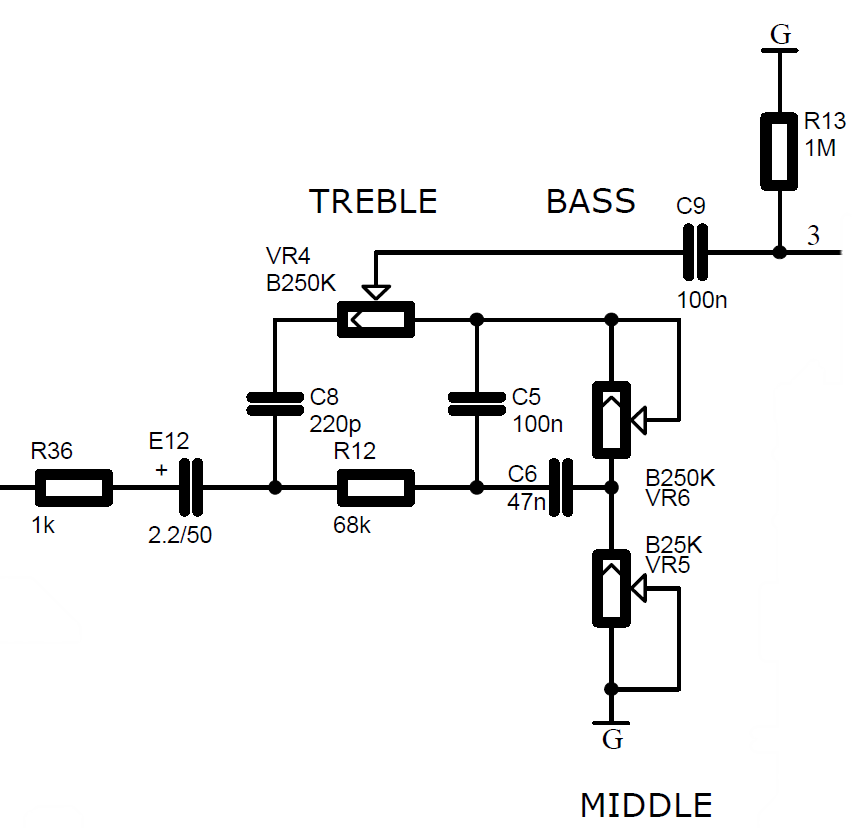
\includegraphics[scale=0.35]{figures/stage4.png}
    \caption{Az erősítő tone stack áramköre}
\end{figure}
Az erősítő tone stack részét is szintén bilineáris transzformáció segítségével modelleztem. Sok nehézséget okozott a sok paraméter (itt három is van, $BASS$, $MID$, $TREBLE$, ráadásul a mintavételi idő is), illetve az, hogy a transzformáció során kiszámolandó értékek számára nem adott elég nagy pontosságot a $float$ típus, emiatt $double$ típust kellett használnom. A transzformált rendszer néhány pólusa olyan közel voltak az egységkörhöz, hogy a potméterek bizonyos állásainál a legközelebbi pólus az egységkörön kívülre esett. Ezt a $double$ típusban való tárolás megoldotta. 

A tone stack rész paraméteres felírása és beprogramozása nagyon körülményes feladat, így ez most nem került megvalósításra, de mindenképpen egy továbbfejlesztési lehetőség.
\section{Aktív szűrő}
\begin{figure}[H]
    \centering
    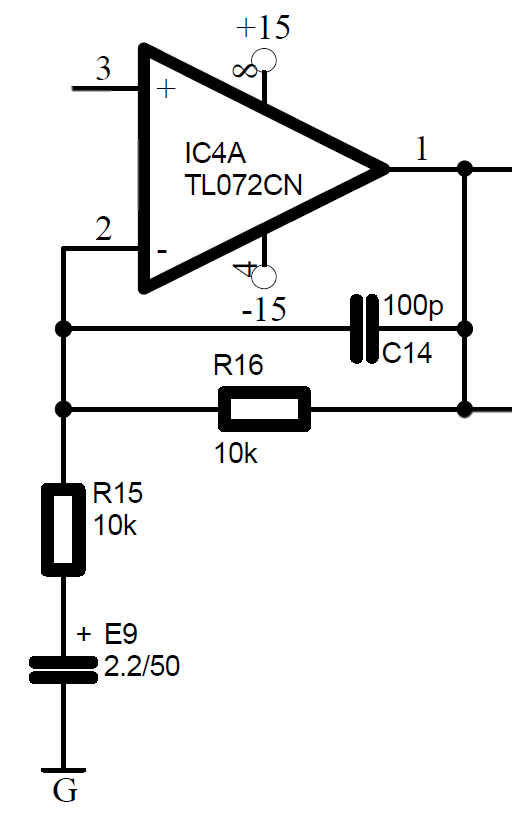
\includegraphics[scale=0.35]{figures/stage5.png}
    \caption{Az erősítő tone stack után lévő aktív szűrő áramkör}
\end{figure}
Egyszerű aktív szűrő, bilineáris transzformáció segítségével modelleztem. Célja az áramkörben, hogy az esetleges mély- és magas frekvenciakomponenseket kiszűrje. A bilineáris transzformáció miatt a mintavételi frekvenciákhoz közeli frekvenciákon nem pontos, hiszen bilineáris transzformáció segítségével modellezett diszkrét rendszer átvitele jelentősen eltérhet az eredeti folytonos idejű rendszer átvitelétől a mintavételi frekvencia közelében.
\begin{figure}[H]
    \centering
    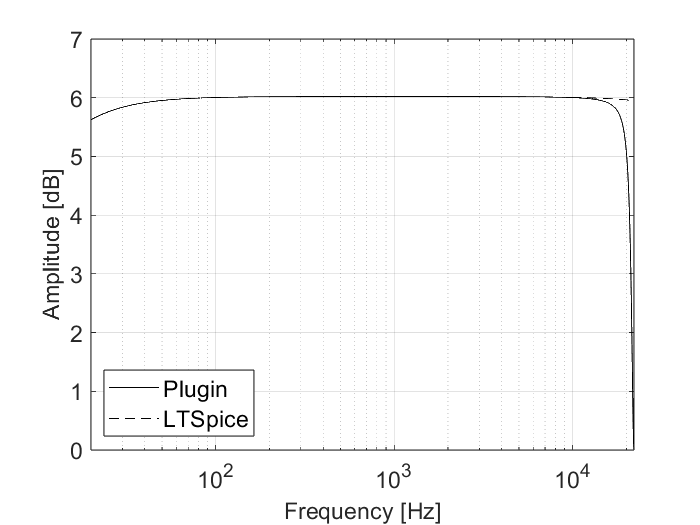
\includegraphics[scale=0.5]{figures/stage5ac.png}
    \caption{Az erősítő tone stack után lévő aktív szűrő áramkörének a modellezett átvitele az eredeti átvitelhez képest}
\end{figure}

\section{Összeadó áramkör}
\begin{figure}[H]
    \centering
    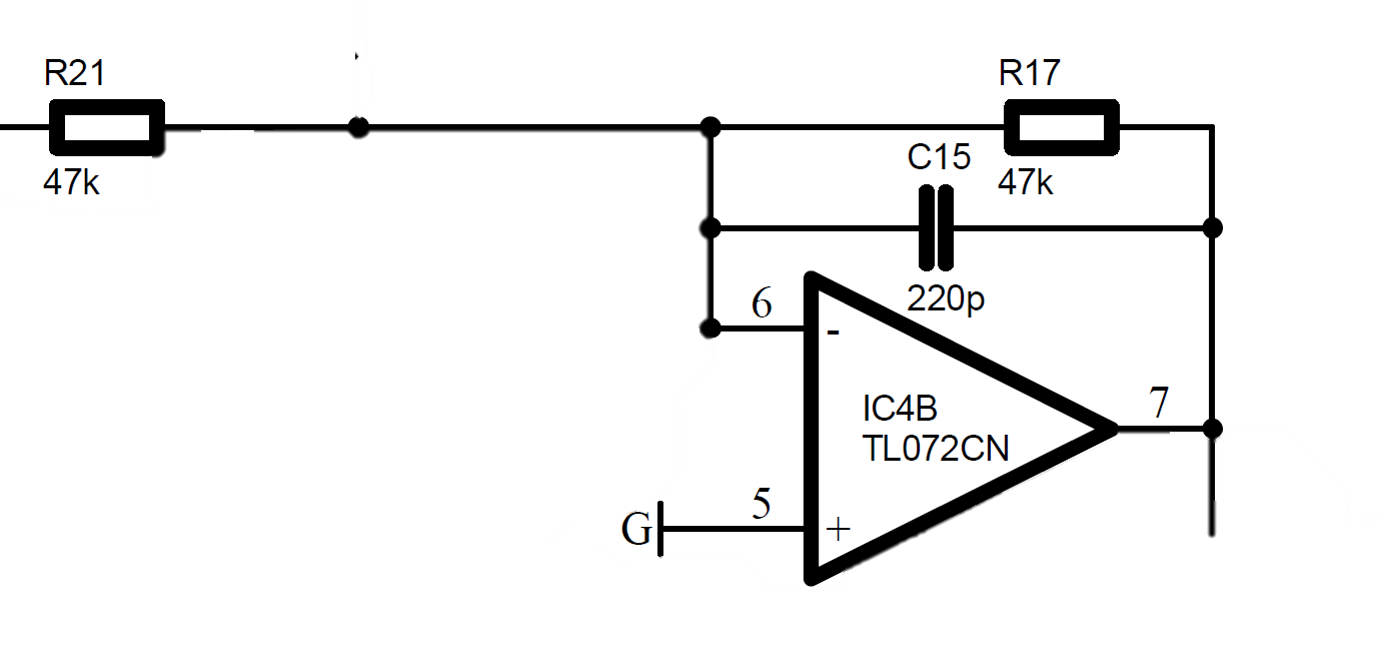
\includegraphics[scale=0.35]{figures/stage6.png}
    \caption{Az áramkör, ami az erősítő jack bemenetén beadott jelet összeadja az erősítő jelével}
\end{figure}

Ez az áramköri rész azért felel, hogy az erősítőbe jack csatlakozón beadott jelet összeadja az erősítő jelével. Mivel a jack csatlakozón beadott jelet nem akarjuk módosítani, ezért minden hangszínváltoztatás és torzítás után van ez az áramkör. Az erősítése egységnyi, és egy aluláteresztő szűrőt valósít meg, hogy a jack bemenetről bejövő nagy frekvenciájú komponenseket kiszűrje. Bilineáris transzformáció segítségével modelleztem.
\begin{figure}[H]
    \centering
    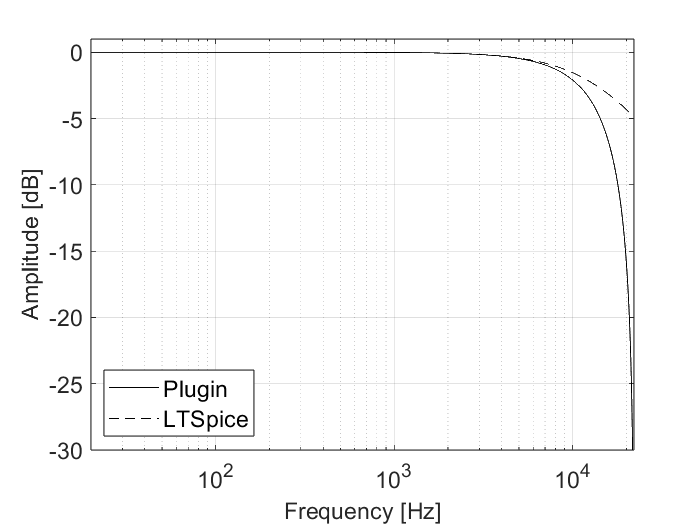
\includegraphics[scale=0.5]{figures/stage6ac2.png}
    \caption{Az áramkör, ami az erősítő jack bemenetén beadott jelet összeadja a gitár jelével}
\end{figure}

\section{Hangerőszabályozó}

\begin{figure}[H]
    \centering
    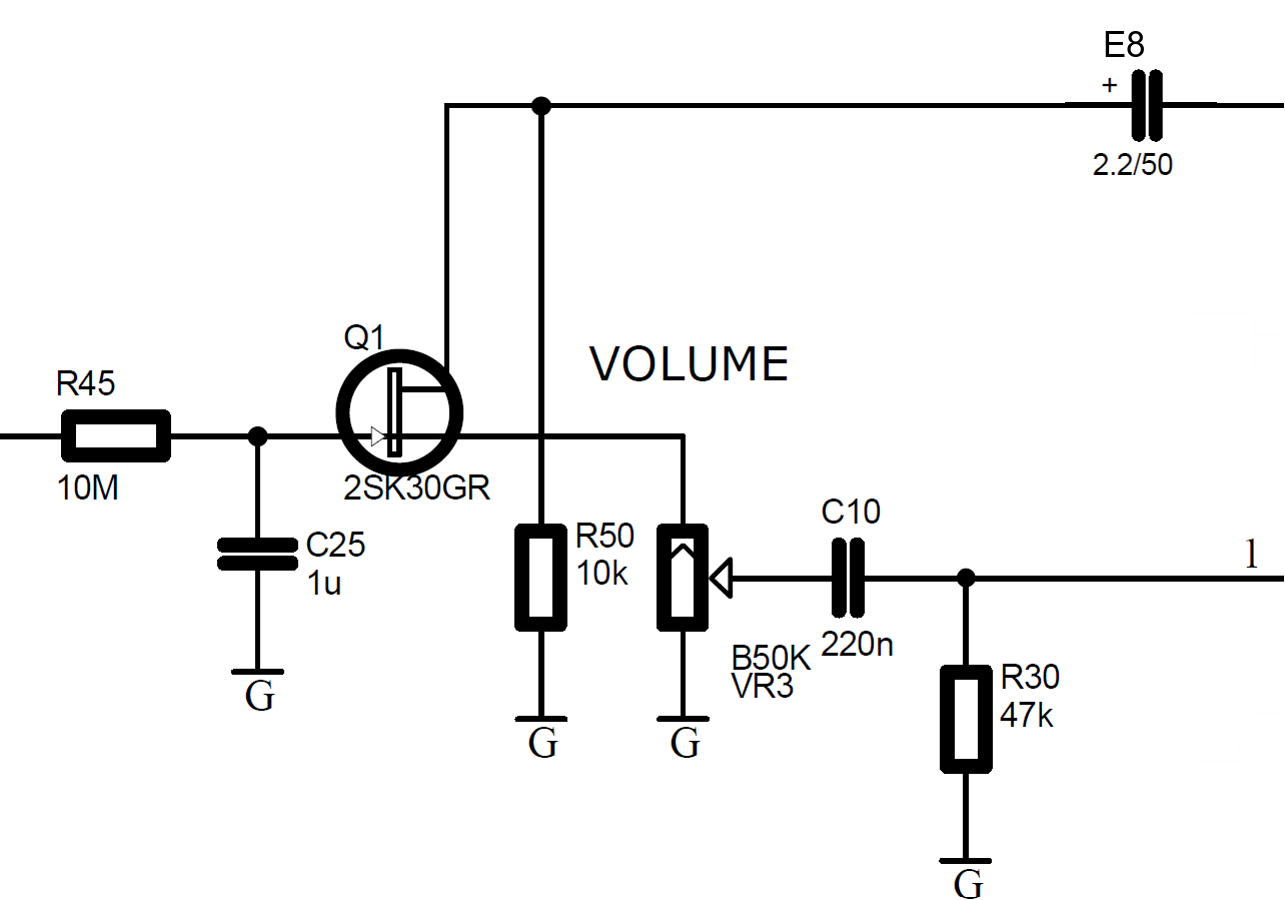
\includegraphics[scale=0.45]{figures/stage7.png}
    \caption{Az erősítő hangerőszabályzó áramköre}
\end{figure}

Az eredeti áramkörben lehet látni egy MOSFET tranzisztort a hangerőszabályzó potméter előtt. Ez a tranzisztor a végfokozat védelmét biztosítja. A MOSFET gate elektródáján lévő $1\mu F$ kapacitású kondenzátor lassan fog feltöltődni az előtte található $10M\Omega$-os ellenálláson. Miután feltöltődött teljesen, utána a MOSFET gate-jén konstans feszültség lesz, nyitva lesz, és az impedanciája az alapján fog változni, amennyi feszültség esik rajta, viszont ez $m\Omega$ nagyságrendekben lesz, ami elhanyagolható az utána lévő $10k\Omega$-os osztó miatt.

A részáramkört szintén bilineáris transzformáció segítségével modelleztem.

\begin{figure}[H]
    \centering
    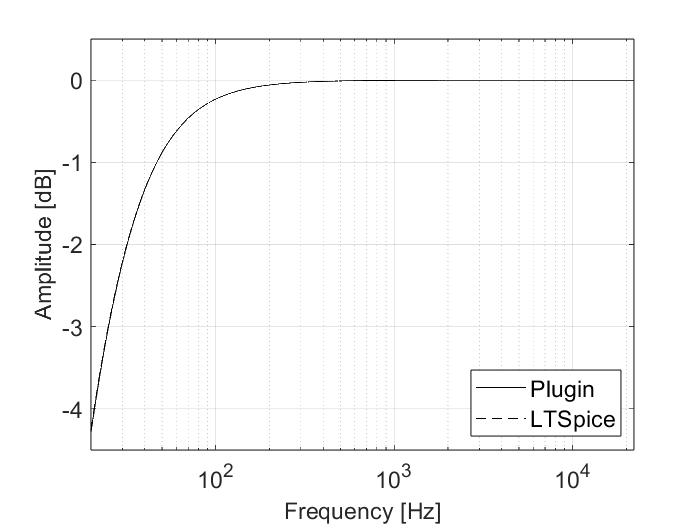
\includegraphics[scale=0.5]{figures/stage7ac3.png}
    \caption{A részáramkör átvitele a VOLUME potméter maximum értéke, azaz $10k\Omega$ mellett}
\end{figure}


\section{Végfokozat}
\begin{figure}[H]
    \centering
    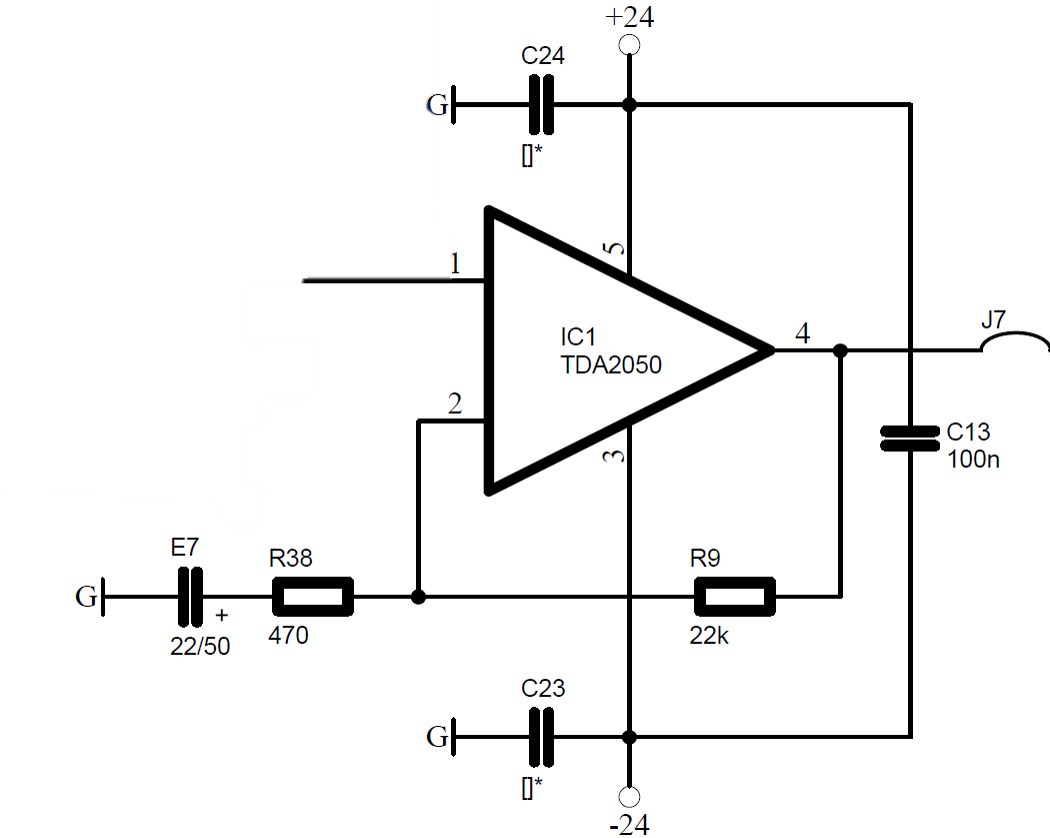
\includegraphics[scale=0.35]{figures/stage8.png}
    \caption{Az erősítő kimenő fokozatának áramköre}
\end{figure}
Ez az áramköri rész gondoskodik arról, hogy az erősítő jelét felerősítse olyan szintre, hogy ezután már csak a hangszóróra kelljen rávezetni. A műveleti erősítő tápján a kondenzátoroknak a tápfeszültség stabilitása a célja, hogy mind a közös módusú, mind pedig a differenciál módusú zavarok ellen védelmet nyújtsanak. Az $E7$ kondenzátornak köszönhetően az átvitelnek felüláteresztő jellege lesz.Ezt az áramköri részt is bilineáris transzformáció segítségével modelleztem. A műveleti erősítő a folytonos idejű áramkörnél levág nagyobb hangerőszinteknél, ez viszont valószínűleg nem cél. Ennek ellenére megvalósítottam ezt is egy egyszerű levágó algoritmussal \cite{opampo}, hogy könnyebben tudjam a plugin hangerőszintjeit skálázni (megfelelő legyen digitális szinteknek).
\begin{figure}[H]
    \centering
    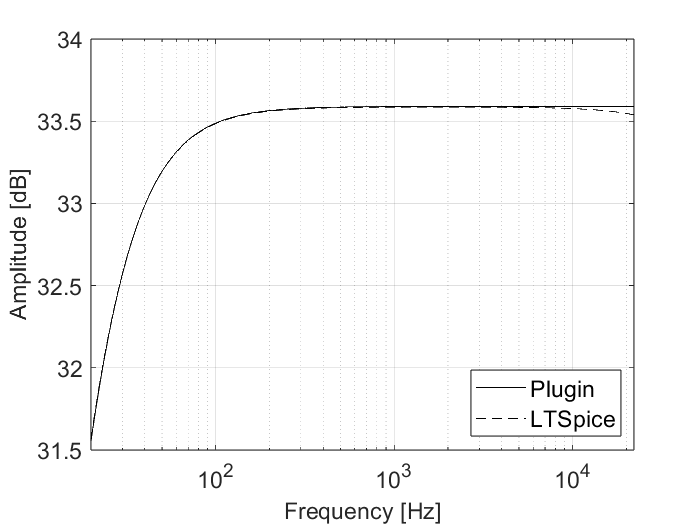
\includegraphics[scale=0.5]{figures/stage8ac.png}
    \caption{Az erősítő kimenő fokozatának áramköre}
\end{figure}
Az átvitelnél a nagy frekvenciáknál valószínűleg azért látható különbség az LTSpice szimuláció és az én megvalósításom között, mert az LTSpice nem ideális műveleti erősítő modellt használ, hanem ilyen nagy erősítéseknél már frekvenciafüggő az átvitele. 




% Acknowledgements
%~~~~~~~~~~~~~~~~~~~~~~~~~~~~~~~~~~~~~~~~~~~~~~~~~~~~~~~~~~~~~~~~~~~~~~~~~~~~~~~~~~~~~~
%%----------------------------------------------------------------------------
\chapter*{\koszonetnyilvanitas}\addcontentsline{toc}{chapter}{\koszonetnyilvanitas}
%----------------------------------------------------------------------------

Ez nem kötelező, akár törölhető is. Ha a szerző szükségét érzi, itt lehet köszönetet nyilvánítani azoknak, akik hozzájárultak munkájukkal ahhoz, hogy a hallgató a szakdolgozatban vagy diplomamunkában leírt feladatokat sikeresen elvégezze. A konzulensnek való köszönetnyilvánítás sem kötelező, a konzulensnek hivatalosan is dolga, hogy a hallgatót konzultálja.


% List of Figures, Tables
%~~~~~~~~~~~~~~~~~~~~~~~~~~~~~~~~~~~~~~~~~~~~~~~~~~~~~~~~~~~~~~~~~~~~~~~~~~~~~~~~~~~~~~
%\listoffigures\addcontentsline{toc}{chapter}{\listfigurename}
%\listoftables\addcontentsline{toc}{chapter}{\listtablename}

% Bibliography
%~~~~~~~~~~~~~~~~~~~~~~~~~~~~~~~~~~~~~~~~~~~~~~~~~~~~~~~~~~~~~~~~~~~~~~~~~~~~~~~~~~~~~~
\nocite{*}
\addcontentsline{toc}{chapter}{\bibname}
\bibliography{bib/mybib.bib}


% Appendix
%~~~~~~~~~~~~~~~~~~~~~~~~~~~~~~~~~~~~~~~~~~~~~~~~~~~~~~~~~~~~~~~~~~~~~~~~~~~~~~~~~~~~~~
%%----------------------------------------------------------------------------
\appendix
%----------------------------------------------------------------------------
\chapter*{\fuggelek}\addcontentsline{toc}{chapter}{\fuggelek}
\setcounter{chapter}{\appendixnumber}
%\setcounter{equation}{0} % a fofejezet-szamlalo az angol ABC 6. betuje (F) lesz
\numberwithin{equation}{section}
\numberwithin{figure}{section}
\numberwithin{lstlisting}{section}
%\numberwithin{tabular}{section}

%----------------------------------------------------------------------------
\section{}
%----------------------------------------------------------------------------


%\label{page:last}
\end{document}
